% Ce fichier main.tex est le fichier principal \`{a} partir duquel tout est g\'{e}n\'{e}r\'{e}
% This file is the main file where the final document is generated
\documentclass{these-dbl}


% Remplir les metadonnees du pdf
% Fill the pdf metadata
\hypersetup{
    pdfauthor   = {Marie Delavergne},
%    pdftitle    = {Th\`{e}se de doctorat de XYZ},
%    pdfsubject  = {Th\`{e}se de doctorat de XYZ},
%    pdfkeywords = {mots-cl\'{e}s},
}

\geometry{vmargin=4.0cm}

\usepackage[utf8]{inputenc}

\usepackage{amsmath,amssymb,amsfonts}


\usepackage{algorithmic}


\usepackage{graphicx}


\usepackage{textcomp}


\usepackage[dvipsnames]{xcolor}


\usepackage{hyperref}
%\renewcommand\UrlFont{\color{MidnightBlue}\rmfamily}
\hypersetup{colorlinks=true, citecolor=RoyalPurple, filecolor=black, linkcolor=BlueViolet, urlcolor=MidnightBlue}

\addto\extrasenglish{
    \def\chapterautorefname{Chapter}
}

\addto\extrasenglish{
    \def\sectionautorefname{Section}
}

\usepackage{xspace}

%% Code highlight
\usepackage{upquote}  % To set `upquote=true` in `lstset`

\usepackage{listings}

\usepackage{enumitem}

\usepackage{verbatim}

\usepackage{wrapfig}
\usepackage{sidecap}
\usepackage{subcaption}

%\usepackage{caption}

%% For background highlight in listing
%% See https://tex.stackexchange.com/a/159602
\newcommand{\hlight}[1]{%
  \colorbox{cyan!10}{#1}%
}

% Listings preferences, with upquote => if we don't use upquote, no need for textcomp either
\lstset{
  basicstyle=\ttfamily\footnotesize,
  upquote=true,
  morecomment=[l]{\#},
  commentstyle=\ttfamily\itshape,
  numbersep=3pt,numberstyle=\ttfamily\tiny,
}



%%   ___          ___
%%  (o o)        (o o)
%% (  V  ) TIKZ (  V  )
%% --m-m----------m-m--

\usepackage{tikz}
\usetikzlibrary{
  positioning, % syntax `below=<optional length> of ...`
  backgrounds, % pgfonlayer{background}
  arrows.meta, % for more arrows options
  matrix,
  fit,
  calc,        % Math operations on coordinate `($s_i+(0,-1mm)$)`
  shapes.geometric,
  shapes.symbols,
}
\usepackage{etoolbox}  % For foreach in matrix

%% Color blind accessible palette
\definecolor{myyellow}{RGB}{255,194,10}
\definecolor{myblue}{RGB}{12,123,220}

%% Tikz Shapes
\tikzset{every picture/.style={node distance=5mm}}
\tikzstyle{app}=[rounded corners, thin, fill=black]
\tikzstyle{labeled}=[minimum size=3mm, inner sep=0pt]
\tikzstyle{endpoint}=[labeled, circle, draw, thin, labeled, minimum size=4mm]
\tikzstyle{client}=[endpoint, fill=black, minimum size=2mm]
\tikzstyle{service}=[matrix of math nodes, draw, row sep=2mm]
\tikzstyle{db}=[cylinder, shape border rotate=90, draw]

% Macro to draw a service with many endpoints and a specific id
% `\service{id}{name}{endpoint_1,endpoint_2,ep_3}'
\newcommand\idservice[4][]{
  %% Build the matrix content outside
  %% https://tex.stackexchange.com/a/22276
  %% Use also \show\mymatrixcontent to see the expansion
  \let\mymatrixcontent\empty
  \expandafter\gappto\expandafter\mymatrixcontent\expandafter{|[draw=none, minimum size=0mm]| #3\\}%
  \foreach \endpoint in {#4} {%
    \expandafter\gappto\expandafter\mymatrixcontent\expandafter{|[endpoint]|}
    \expandafter\gappto\expandafter\mymatrixcontent\expandafter{\endpoint\\}
  }

  \matrix (#2) [service,#1] {\mymatrixcontent};
}

% Service with same name and id,
% `\service{name}{endpoint_1,endpoint_2,ep_3}'
\newcommand\service[3][]{\idservice[#1]{#2}{#2}{#3}}
% Service mesh with id, service mesh
\newcommand\idmesh[4][]{\idservice[dashed,draw=none,#1]{#2}{#3}{#4}}
\newcommand\mesh[3][]{\idmesh[#1]{#2}{#2}{#3}}

%%   ___              ___
%%  (o o)            (o o)
%% (  V  ) END_TIKZ (  V  )
%% --m-m--------------m-m--

%% Hyphenation
%% TeX won't hyphenate a word that's already been hyphenated. For
%% example, "geo-distributed". Replace the hyphen in the
%% "geo-distributed" with a \hyph command `geo\hyph{}distributed`.
%% See https://www.texfaq.org/FAQ-nohyph
\def\hyph{-\penalty0\hskip0pt\relax}
\hyphenation{geo-dis-tri-bu-tion geo-dis-tri-bu-ted Dev-Ops}


\usepackage[textwidth=17mm, colorinlistoftodos]{todonotes}


\definecolor{CbBlue}{HTML}{332288}
\definecolor{CbGreen}{HTML}{117733}
\definecolor{CbTeal}{HTML}{44aa99}
\definecolor{CbCyan}{HTML}{88ccee}
\definecolor{CbOrange}{HTML}{ffab40}
\definecolor{CbRose}{HTML}{cc6677}
\definecolor{CbFuschia}{HTML}{aa4499}
\definecolor{CbPlum}{HTML}{882255}

\newcommand{\tododo}[1]{\todo[inline, shadow, color=CbTeal!80]{#1}}
\newcommand{\todoref}[1]{\todo[inline, shadow, color=SeaGreen!80]{#1}}
\newcommand{\todomore}[1]{\todo[inline, shadow, color=RoyalPurple!40]{#1}}
\newcommand{\todocheck}[1]{\todo[inline, shadow, color=Yellow!40]{#1}}
\newcommand{\todono}[1]{\todo[inline, shadow, color=OrangeRed!80]{#1}}
\newcommand{\todofig}[1]{\missingfigure[figcolor=white]{#1}}


% colored cite brackets
\DeclareOuterCiteDelims{cite}{\textcolor{RoyalPurple}{\bibopenbracket}}{\textcolor{RoyalPurple}{\bibclosebracket}}


\usepackage{epigraph}
%\usepackage{epipart}

%\usepackage[printonlyused,withpage]{acronym}

\usepackage[acronym,toc]{glossaries}
% https://tex.stackexchange.com/questions/198231/remove-page-break-before-glossary
\renewcommand*{\glsclearpage}{}

\newglossarystyle{better}{%
  \glossarystyle{list}%
  \renewcommand*{\glossaryentryfield}[5]{%
    \item[\glsentryitem{##1}\glstarget{##1}{##2}] ##3%
      }%
  \renewcommand*{\glsgroupskip}{}%
}

\glossarystyle{better}


\newcommand{\eg}{{e.g.,}\xspace}
\newcommand{\ie}{{i.e.,}\xspace}
\newcommand{\scl}{scope-lang\xspace}
\newcommand{\os}{OpenStack\xspace}
\newcommand{\ks}{Kubernetes\xspace}
\newcommand{\sOne}{Site~1\xspace}
\newcommand{\sTwo}{Site~2\xspace}
\newcommand{\collab}{collaboration}
\newcommand{\mscl}{\mathit{Scope}}
\newcommand{\mscll}[1]{\mathit{Scope}=\mathit{#1}}
\newcommand{\dc}{\gls{dc}\xspace}
\newcommand{\dcs}{\glspl{dc}\xspace}
\newcommand{\Dc}{Data center\xspace}
\newcommand{\Dcs}{Data centers\xspace}


\usepackage{multirow}

\usepackage{tcolorbox}

% Spécifier vos fichiers de bibliographie
% Specify you bibliography files here
\addbibresource{./biblio/biblio.bib}

% Generate the glossary
%
\newglossaryentry{service}
{
name={Service},
text={service},
description={A service consists in a set of functionalities, typically
using one or a few different resources, which allows a complete
business goal. For example, a billing service, a user management
service, in a shopping application}
}

\newglossaryentry{DevOps}
{
name={DevOps},
description={DevOps is a
portmanteau word composed of (software) development and (IT)
operations. DevOps are mainly a set of practices that combines those
in order to produce faster better products for customers. Globally, it
enhances the application lifecycle through methods used during the
lifecycle phases, plan, develop, deliver and operate.}
}

\newglossaryentry{p2p} {
name={Peer-to-peer},
text={peer-to-peer},
description={Peer-to-peer
computing is a type of architecture for distributed applications to
spread their workloads between peers of the system on which it is
deployed upon. Peers all have the same privileges and same function
abilities.}
}

\newglossaryentry{tls} {
name={Transport Layer Security},
description={TLS is a security protocol that provides secured and private
communications in computer networks. It used for HTTPS, but also emails,
instant messaging, etc.}
}


\newglossaryentry{api} {
name={Application Programming Interface},
description={An API is a software interface allowing other programs to
interact with the software functionalities that are exposed by this interface.
One of the goals is to keep the software internals hidden and expose only what
is relevant for software communications.}
}

\newglossaryentry{server} {
name={Server},
text={server},
description={A server is a \emph{computer} designed to process requests,
offer functionalities and deliver data to other, possibly multiple softwares or
devices that are called clients.}  }

\newglossaryentry{dc} {
name={Data center},
text={data center},
description={A data center
is a physical facility hosting networked computing and storage
components.}
}

\newglossaryentry{udp} {
name={User Datagram Protocol},
description={UDP is one of the communication protocol over IP network. Contrary to TCP, UDP does not require to establish a connection between the client and the server.}
}

\newglossaryentry{tcp} {
name={Transmission Control Protocol},
description={TCP is one of the main communication protocol,
complemented by the IP (Internet Protocol). TCP is based on the
establishment of a connection between the client and the server before
data are sent to deliver reliable data streams.}
}

\newglossaryentry{iot} {
name={Internet of things},
description={The internet of things consists in physical devices that carry sensors, have processing capabilities, and different technologies, to connect to other devices and computing systems, not necessarily on the internet. For examples, smart homes can be composed of different devices that compose the internet of things, like cameras, thermostats, etc.}
}


\newglossaryentry{router} {
name={Router},
text={router},
description={A router is a network device dedicated to forwarding data packets between networks. On the internet, they direct the traffic where it is needed.}
}

\newglossaryentry{switch} {
name={Switch},
text={switch},
description={A switch is a network device dedicated to forwarding data between the devices connected to it.}
}

% HERE

\newglossaryentry{disk array} {
name={Disk array},
text={disk array},
description={A disk array is a set of disk drives that compose a disk storage system.}
}

\newglossaryentry{loosely coupled} {
name={Loosely coupled},
text={loosely coupled},
description={Loose coupling refers to a model where the components of the system are connected but not heavily dependent, so they are not affected by changes or failures of others.}
}

\newglossaryentry{Contentdn} {
name={Content Delivery Network},
description={CDNs are a layer in the internet ecosystem. They consist in geo-distributed networks of data centers that delivers content (such as images, softwares, videos, streaming media, etc.) to end-users by being close to them. For example, Netflix or Youtube use CDN in most countries to deliver their videos faster.}
}

\newglossaryentry{cache} {
name={Cache},
text={cache},
description={A cache is a component that stores data closer to its usage point so future requests on this data will be served faster. For example, your browser saves logos or images of website so it does not need to download them again next time you are navigating them.}
}

\newglossaryentry{Domainns} {
name={Domain Name System},
description={The DNS is a naming system used to identify computers by a human friendly domain name by mapping it to IP addresses. For example, 8.8.8.8 is the primary DNS server for Google DNS.}
}

\newglossaryentry{cloudlet} {
name={Cloudlet},
text={cloudlet},
description={A cloudlet is a small-scale data center that is mobile at the edge of the internet.}
}

\newglossaryentry{smart contract} {
name={Smart contract},
text={smart contract},
description={A smart contract is a class of computer protocol that allows, check and execute the actions required by the terms of a contract. The main idea is to have automated agreements to ensure the terms of smart contract terms depending of predetermined factors.}
}

\newglossaryentry{hypervisor} {
name={Hypervisor},
text={hypervisor},
description={A hypervisor is a software that can create and run virtual machines (virtualization of computer systems).}
}

\newglossaryentry{microservice} {
name={Microservice},
text={microservice},
description={The microservice architecture is an architectural style that composes an application as a collection of services thatare loosely coupled, deployable independently, and execute each a small and coherent part of the business functions.}
}

\makeglossaries
\loadglsentries{./glossary}
\loadglsentries{./acronym}

\begin{document}



% Page de garde avec commande \maketitle
% Front cover calling \maketitle
% La page de garde est en français
% The front cover is in French
\selectlanguage{french}

% Inclure les infos de chaque établissement
% Include each institution data

%%% Switch case in latex
%%% https://tex.stackexchange.com/a/343306
\makeatletter
\newcommand\addcase[3]{\expandafter\def\csname\string#1@case@#2\endcsname{#3}}
\newcommand\makeswitch[2][]{%
  \newcommand#2[1]{%
    \ifcsname\string#2@case@##1\endcsname\csname\string#2@case@##1\endcsname\else#1\fi%
  }%
}
\makeatother

%%%% Il faut adapter la taille des logos dans certains cas (e.g., EGAAL, 2 etablissements)
\newcommand\hauteurlogos[3]{
    \hauteurlogoecole{#1}
    \hauteurlogoetablissementA{#2}
    \hauteurlogoetablissementB{#3}
}

%%%%%%%%%%%%%%%%%%%%%%%%%%%%%%%%%%%%%%%%%%%%%%%%%%%
%%%%%%%%%%%%%%%% ECOLES DOCTORALES %%%%%%%%%%%%%%%%

%%%% #1: dossier des images, #2: numero ED, #3: couleur ED, #4-#5: nom complet sur plusieurs lignes
\newcommand\addecoledoctorale[5]{\direcole{#1}\numeroecole{#2}\definecolor{color-ecole}{RGB}{#3}\nomecoleA{#4}\nomecoleB{#5}}

\makeswitch[default]\ecoledoctorale{}

\addcase\ecoledoctorale{3M}{\addecoledoctorale
    {3M}
    {596}
    {193,192,183}
    {Mati\`{e}re, Mol\'{e}cules, Mat\'{e}riaux}
    {}
}
\addcase\ecoledoctorale{ALL}{\addecoledoctorale
    {ALL}
    {595}
    {240,209,134}
    {Arts, Lettres, Langues}
    {}
}
\addcase\ecoledoctorale{BS}{\addecoledoctorale
    {BS}
    {605}
    {163,219,208}
    {Biologie, Sant\'{e}}
    {}
}
\addcase\ecoledoctorale{DSP}{\addecoledoctorale
    {DSP}
    {599}
    {188,208,220}
    {Droit et Science politique}
    {}
}
\addcase\ecoledoctorale{EDGE}{\addecoledoctorale
    {EDGE}
    {597}
    {216,178,210}
    {Sciences \'{E}conomiques et sciences De Gestion}
    {}
}
\addcase\ecoledoctorale{EGAAL}{\addecoledoctorale
    {EGAAL}
    {600}
    {146,213,182}
    {\'{E}cologie, G\'{e}osciences, Agronomie et Alimentation}
    {}
    \hauteurlogos{2cm}{2cm}{2cm}
}
\addcase\ecoledoctorale{ELICC}{\addecoledoctorale
    {ELICC}
    {603}
    {249,201,188}
    {\'{E}ducation, Langages, Interactions, Cognition, Clinique}
    {}
    \hauteurlogos{2cm}{2cm}{2cm}
}
\addcase\ecoledoctorale{MathSTIC}{\addecoledoctorale
    {MathSTIC}
    {648}
    {79,92,162}
    {Sciences Pour l'Ingénieur et le Numérique}
    {}
}
\addcase\ecoledoctorale{SML}{\addecoledoctorale
    {SML}
    {598}
    {162,225,230}
    {Sciences de la Mer et du Littoral}
    {}
}
\addcase\ecoledoctorale{SPI}{\addecoledoctorale
    {SPI}
    {602}
    {159,182,217}
    {Sciences pour l'Ing\'{e}nieur}
    {}
}
\addcase\ecoledoctorale{STT}{\addecoledoctorale
    {STT}
    {604}
    {172,184,192}
    {Soci\'{e}t\'{e}s, temps, territoires}
    {}
}



%%%%%%%%%%%%%%%%%%%%%%%%%%%%%%%%%%%%%%%%%%%%%%%%
%%%%%%%%%%%%%%%% ETABLISSEMENTS %%%%%%%%%%%%%%%%

%%%% #1 nom du logo, #2-#4: nom complet sur plusieurs lignes
\newcommand\addetablissement[4]{\logoetablissementB{#1}\nometablissementC{#2}\nometablissementD{#3}\nometablissementE{#4}}

\makeswitch[default]\etablissement{}

\addcase\etablissement{CS}{\addetablissement
    {CS}
    {}
    {}
    {CENTRALESUP\'{E}LEC}
}
\addcase\etablissement{ECN}{\addetablissement
    {ECN}
    {}
    {}
    {L'\'{E}COLE CENTRALE DE NANTES}
}
\addcase\etablissement{EHESP}{\addetablissement
    {EHESP}
    {}
    {L'\'{E}COLE DES HAUTES \'{E}TUDES}
    {EN SANT\'{E} PUBLIQUE DE RENNES}
}
\addcase\etablissement{ENIB}{\addetablissement
    {ENIB}
    {}
    {L'\'{E}COLE NATIONALE}
    {D'ING\'{E}NIEURS DE BREST}
}
\addcase\etablissement{ENS}{\addetablissement
    {ENS}
    {}
    {L'\'{E}COLE NORMALE}
    {SUP\'{E}RIEURE RENNES}
}
\addcase\etablissement{ENSA}{\addetablissement
    {ENSA}
    {}
    {L'\'{E}COLE NORMALE SUP\'{E}RIEURE}
    {D'ARCHITECTURE DE NANTES}
}
\addcase\etablissement{ENSAB}{\addetablissement
    {ENSAB}
    {}
    {L'\'{E}COLE NORMALE SUP\'{E}RIEURE}
    {D'ARCHITECTURE DE BRETAGNE}
}
\addcase\etablissement{ENSAI}{\addetablissement
    {ENSAI}
    {}
    {L'\'{E}COLE NATIONALE DE LA STATISTIQUE}
    {ET DE L'ANALYSE DE L'INFORMATION}
}
\addcase\etablissement{ENSCR}{\addetablissement
    {ENSCR}
    {}
    {L'\'{E}COLE NATIONALE SUP\'{E}RIEURE}
    {DE CHIMIE RENNES}
}
\addcase\etablissement{ENSTA}{\addetablissement
    {ENSTA}
    {}
    {L'\'{E}COLE NATIONALE SUP\'{E}RIEURE}
    {DE TECHNIQUES AVANC\'{E}ES BRETAGNE}
}
\addcase\etablissement{IMTA}{\addetablissement
    {IMTA}
    {L'\'{E}COLE NATIONALE SUP\'{E}RIEURE}
    {MINES-T\'{E}L\'{E}COM ATLANTIQUE BRETAGNE}
    {PAYS-DE-LA-LOIRE - IMT ATLANTIQUE}
}
\addcase\etablissement{INSA}{\addetablissement
    {INSA}
    {}
    {L'INSTITUT NATIONAL DES}
    {SCIENCES APPLIQU\'{E}ES RENNES}
}
\addcase\etablissement{InstitutAgro}{\addetablissement
    {InstitutAgro}
    {L'INSTITUT NATIONAL D'ENSEIGNEMENT SUP\'{E}RIEUR}
    {POUR L'AGRICULTURE, L'ALIMENTATION ET}
    {L'ENVIRONNEMENT - ECOLE INTERNE AGROCAMPUS OUEST}
}
\addcase\etablissement{LMU}{\addetablissement
    {LMU}
    {}
    {}
    {LE MANS UNIVERSIT\'{E}}
}
\addcase\etablissement{Oniris}{\addetablissement
    {Oniris}
    {}
    {}
    {ONIRIS}
}
\addcase\etablissement{UA}{\addetablissement
    {UA-couleur}
    {}
    {}
    {L'UNIVERSIT\'{E} D'ANGERS}
}
\addcase\etablissement{UB}{\addetablissement
    {UB}
    {}
    {}
    {L'UNIVERSIT\'{E} DE BREST}
}
\addcase\etablissement{UBO}{\addetablissement
    {UBO}
    {}
    {}
    {L'UNIVERSIT\'{E} DE BRETAGNE OCCIDENTALE}
}
\addcase\etablissement{UBS}{\addetablissement
    {UBS}
    {}
    {}
    {L'UNIVERSIT\'{E} DE BRETAGNE SUD}
}
\addcase\etablissement{UN}{\addetablissement
    {UN-noir}
    {}
    {}
    {L'UNIVERSIT\'{E} DE NANTES}
}
\addcase\etablissement{UR1}{\addetablissement
    {UR1-noir}
    {}
    {}
    {L'UNIVERSIT\'{E} DE RENNES 1}
}
\addcase\etablissement{UR2}{\addetablissement
    {UR2}
    {}
    {}
    {L'UNIVERSIT\'{E} DE RENNES 2}
}


%%%% #1-#2: nom des deux logos, #3-#7: nom complet de la double affiliation sur plusieurs lignes
\newcommand\addpairetablissements[7]{
    \logoetablissementA{#1}
    \logoetablissementB{#2}
    \nometablissementA{#3}
    \nometablissementB{#4}
    \nometablissementC{#5}
    \nometablissementD{#6}
    \nometablissementE{#7}
}

% ALL, STT: UR2-ENSAB
\addcase\etablissement{UR2-ENSAB}{\addpairetablissements
    {ENSAB}
    {UR2}
    {}
    {L'\'{E}COLE NORMALE SUP\'{E}RIEURE}
    {D'ARCHITECTURE DE BRETAGNE}
    {D\'{E}LIVR\'{E}E CONJOINTEMENT AVEC}
    {L'UNIVERSIT\'{E} DE RENNES 2}
    \hauteurlogos{2cm}{1.2cm}{2cm}
}
% BS, DSP, MathSTIC: UR1-UR2
\addcase\etablissement{UR1-UR2}{\addpairetablissements
    {UR2}
    {UR1-noir}
    {}
    {}
    {L'UNIVERSIT\'{E} DE RENNES 2}
    {D\'{E}LIVR\'{E}E CONJOINTEMENT AVEC}
    {L'UNIVERSIT\'{E} DE RENNES 1}
    \hauteurlogos{2cm}{2cm}{2cm}
}
% DSP, EDGE: UR1-EHESP
\addcase\etablissement{UR1-EHESP}{\addpairetablissements
    {EHESP}
    {UR1-noir}
    {}
    {L'UNIVERSIT\'{E} DE RENNES 1}
    {D\'{E}LIVR\'{E}E CONJOINTEMENT AVEC}
    {L'\'{E}COLE DES HAUTES \'{E}TUDES}
    {EN SANT\'{E} PUBLIQUE DE RENNES}
    \hauteurlogos{2cm}{2cm}{2cm}
}
% EGAAL: UA-LMU
\addcase\etablissement{UA-LMU}{\addpairetablissements
    {LMU}
    {UA-couleur}
    {}
    {}
    {LE MANS UNIVERSIT\'{E}}
    {D\'{E}LIVR\'{E}E CONJOINTEMENT AVEC}
    {L'UNIVERSIT\'{E} D'ANGERS}
    \hauteurlogos{2cm}{1cm}{2cm}
}
% MathSTIC: UR1-InstitutAgro
\addcase\etablissement{UR1-InstitutAgro}{\addpairetablissements
    {InstitutAgro}
    {UR1-noir}
    {L'INSTITUT NATIONAL D'ENSEIGNEMENT SUP\'{E}RIEUR}
    {POUR L'AGRICULTURE, L'ALIMENTATION ET}
    {L'ENVIRONNEMENT - ECOLE INTERNE AGROCAMPUS OUEST}
    {D\'{E}LIVR\'{E}E CONJOINTEMENT AVEC}
    {L'UNIVERSIT\'{E} DE RENNES 1}
    \hauteurlogos{1.8cm}{1.3cm}{1.5cm}
}
% SML: UBO-IMTA
\addcase\etablissement{UBO-IMTA}{\addpairetablissements
    {IMTA}
    {UBO}
    {L'\'{E}COLE NATIONALE SUP\'{E}RIEURE}
    {MINES-T\'{E}L\'{E}COM ATLANTIQUE BRETAGNE}
    {PAYS-DE-LA-LOIRE - IMT ATLANTIQUE}
    {D\'{E}LIVR\'{E}E CONJOINTEMENT AVEC}
    {L'UNIVERSIT\'{E} DE BRETAGNE OCCIDENTALE}
    \hauteurlogos{2cm}{1.8cm}{1.8cm}
}
% SPI: ECN-ENSA
\addcase\etablissement{ECN-ENSA}{\addpairetablissements
    {ENSA}
    {ECN}
    {}
    {L'\'{E}COLE NORMALE SUP\'{E}RIEURE}
    {D'ARCHITECTURE DE NANTES}
    {D\'{E}LIVR\'{E}E CONJOINTEMENT AVEC}
    {L'\'{E}COLE CENTRALE DE NANTES}
    \hauteurlogos{2cm}{1.8cm}{1.8cm}
}
% SPI: UBO-ENIB
\addcase\etablissement{UBO-ENIB}{\addpairetablissements
    {ENIB}
    {UBO}
    {}
    {L'\'{E}COLE NATIONALE}
    {D'ING\'{E}NIEURS DE BREST}
    {D\'{E}LIVR\'{E}E CONJOINTEMENT AVEC}
    {L'UNIVERSIT\'{E} DE BRETAGNE OCCIDENTALE}
    \hauteurlogos{2cm}{1.8cm}{1.6cm}
}
% SPI: UN-Oniris
\addcase\etablissement{UN-Oniris}{\addpairetablissements
    {Oniris}
    {UN-noir}
    {}
    {}
    {ONIRIS}
    {D\'{E}LIVR\'{E}E CONJOINTEMENT AVEC}
    {L'UNIVERSIT\'{E} DE NANTES}
    \hauteurlogos{2cm}{2cm}{2cm}
}
% STT: ENSA-UN
\addcase\etablissement{ENSA-UN}{\addpairetablissements
    {ENSA}
    {UN-noir}
    {}
    {L'\'{E}COLE NORMALE SUP\'{E}RIEURE}
    {D'ARCHITECTURE DE NANTES}
    {D\'{E}LIVR\'{E}E CONJOINTEMENT AVEC}
    {L'UNIVERSIT\'{E} DE NANTES}
    \hauteurlogos{2cm}{2cm}{2cm}
}


% Inclure infos de l'école doctorale
% Include doctoral school data
% (3M ALL BS DSP EDGE EGAAL ELICC MathSTIC SML SPI STT)
\ecoledoctorale{MathSTIC}

% Inclure infos de l'établissement
% Include institution data
\etablissement{IMTA}


%Inscrivez ici votre sp\'{e}cialit\'{e} (voir liste des sp\'{e}cialit\'{e}s sur le site de votre \'{e}cole doctorale)
%Indicate the domain (see list of domains in your ecole doctorale)
\spec{Informatique}

%Attention : le pr\'{e}nom doit être en minuscules (Jean) et le NOM en majuscules (BRITTEF)
%Attention : the first name in small letters and the name in Capital letters
\author{Marie DELAVERGNE}

% Donner le titre complet de la th\`{e}se, \'{e}ventuellement le sous titre, si n\'{e}cessaire sur plusieurs lignes
%Give the complete title of the thesis, if necessary on several lines
\title{Cheops, a service-mesh to geo-distribute micro-service applications at the Edge.}
\lesoustitre{A focus on the replication collaboration}

%Indiquer la date et le lieu de soutenance de la th\`{e}se
%indicates the date and the place of the defense
\date{16 mars 2023}
\lieu{l'IMT Atlantique, Amphithéâtre Besse}

%Indiquer le nom du (ou des) laboratoire (s) dans le(s)quel(s) le travail de th\`{e}se a \'{e}t\'{e} effectu\'{e}, indiquer aussi si souhait\'{e} le nom de la (les) facult\'{e}(s) (UFR, \'{e}cole(s), Institut(s), Centre(s)...), son (leurs) adresse(s)...
%Indicates the name (or names) of research laboratories where the work has been done as well as (if desired) the names of faculties (UFR, Schools, institution...
\uniterecherche{Laboratoire des Sciences du Numérique de Nantes (LS2N)}

%Indiquer le Numero de th\`{e}se, si cela est opportun, ou laisser vide pour faire disparaitre cet ligne de la couverture
%Indicate the number of the thesis if there is one. otherwise leave empty so the line disappeurs on the cover
\numthese{2023IMTA0347} % \numthese{}

%Indiquer le Pr\'{e}nom en minuscules et le Nom en majuscules, le titre de la personne et l’\'{e}tablissement dans lequel il effectue sa recherche
%Indicates the first name on small letters and the Names on capital letters, the person's title and the institution where he/she belongs to.
%Exemples :  Examples :
%%%- Professeur, Universit\'{e} d’Angers
%%%- Chercheur, CNRS, \'{e}cole Centrale de Nantes
%%%-  Professeur d’universit\'{e} – Praticien Hospitalier, Universit\'{e} Paris V
%%%-  Maitre de conf\'{e}rences, Oniris
%%%- Charg\'{e} de recherche, INSERM, HDR, Universit\'{e} de Tours
 %S’il n’y a pas de co-direction, faire disparaitre cet item de la couverture
 %In there is no co-director, remove the item from the cover
\jury{
{\normalTwelve \textbf{Rapporteurs avant soutenance :}}\\ \newline
\footnotesizeTwelve
\begin{tabular}{@{}ll}
Noël DE PALMA & Professeur, Université Grenoble Alpes \\
Pierre SENS & Professeur, Sorbonne Université \\
\end{tabular}

\vspace{\baselineskip}
{\normalTwelve \textbf{Composition du Jury :}}\\
% {\fontsize{9.5}{11}\selectfont {\textcolor{red}{\textit{Attention, en cas d’absence d’un des membres du Jury le jour de la soutenance, la composition du jury doit être revue pour s’assurer qu’elle est conforme et devra être répercutée sur la couverture de thèse}}}}\\
\newline
\footnotesizeTwelve
\begin{tabular}{@{}lll}


Pr\'{e}sident : & Thomas LEDOUX & Professeur, IMT Atlantique \\
Examinateurs :         & Sara BOUCHENAK & Professeure, INSA Lyon  \\
& Ronan-Alexandre CHERRUEAU & Administrateur Cloud, Direction Générale des Finances Publiques \\
& Noël DE PALMA & Professeur, Université Grenoble Alpes \\
& Pierre SENS & Professeur, Sorbonne Université \\
Dir. de th\`{e}se :    & Adrien LEBRE & Professeur, IMT Atlantique \\
\end{tabular}

\vspace{\baselineskip}
% {\normalTwelve \textbf{Invit\'{e}(s) :}}\\ \newline
% \footnotesizeTwelve
% \begin{tabular}{@{}ll}
% Pr\'{e}nom NOM & Fonction et \'{e}tablissement d'exercice \\
% \end{tabular}
}


\maketitle


% Sélectionner la langue du contenu suivant cette ligne
% Select the content language following this line
\selectlanguage{english}

% Inclusion du chapitre remerciement
% Input acknowledgement chapter
\clearemptydoublepage
\chapter*{Acknowledgment}

There are a lot of people to thank for my work in my thesis.
%
A lot of really great persons, who taught me a lot, whether it was
directly related to my work, or for transversal knowledge.
%
At some point, I might not be able to describe how useful they were
and how lucky I was to talk with them, in good enough terms, but I
will try anyway.

First of all, I would like to thank my
supervisors.
%
Adrien Lebre, my ``official'' supervisor, was the one to pull me into
this great adventure that is a PhD thesis.
%
I saw firsthand how difficult it can be, and I would never have gotten
into it with anyone else.
%
I knew how dedicated he is with his other PhD students, and though it
was not always easy, of course, he helped and supported me however he
could, and pushed me whenever needed to give my best in my work.
%
Ronan-Alexandre Cherrueau, who definitely was my supervisor even
though it never was official, for the first year and a half.
%
Thanks for your really good ideas, pedagogy, and support.

I would also like to thank everyone in my defense jury, Sara
Bouchenak, Noël De Palma, Thomas Ledoux and Pierre Sens, first for
their time and second for their great questions and remarks during my
defense.

Then, all the people who participated in the project at some point.
%
Matthieu Simonin and Javier Rojas Balderrama, for Openstackoïd and all
the huge help in the beginning of my thesis.
%
David Espinel Sarmiento, with his thesis which initiated the Cross
collaboration, and great input on how it works, and a great partner in
sea kayak.
%
Karim Manaouil and Rodolfo, who participated in the Cheops meetings we
had in spring 2021.
%
Especially thanks to Karim with his help on Kubernetes and Cross and
always had a great perspective on different things.
%
My interns from spring 2021, Matthieu Juzdzewski and Arnaud Szymanek,
who were a great help to understand Consul and how Cheops should be
implemented, and were really great to supervise.
%
Last, but definitely not least, Geo Johns Antony, for all his great
knowledge and input, his patience, and the draft of the collaboration
model.
%
I wish him all the best for the end of his own thesis, even though I
am going to be around to try and help.


Then comes the people from the STACK team.
%
I will try to avoid thanking everyone by name, but some stand out.
%
Anthony Simonet, who took me as his intern one day, and was a great
supervisor and a huge help.
%
Johnathan Pastor, for his work on ROME, without which I would not have
been in the team either, who was always a good friend and a really
nice person, with insightful knowledge that helped a lot during all
these years.
%
Thuy Linh Nguyen and Jad Darrous, who were not only friends, but
convinced me someday to pursue a PhD thesis.
%
Hélène Coullon who was always a good friend too, and one of the nicest
person I had the chance to meet.
%
Maverick Chardet, Émile Cadorel, Fatima-Zahra Boujdad also need to be
thanked, and more recently, Antoine Omond and Baptiste Jonglez.


I am not going to mention every single one of my teachers, but I would
like to thank them anyway.
%
In particular, I would like to thank my university teachers from my
first Licence in Université du Havre Fabrice Durand and Véronique Jay
and of course all of my teachers in my computer science degrees from
Université de Nantes, with a special mention to Florian Richoux,
Frédéric Goualard and Hala Skaf-Molli who really inspired me during
the long road to PhD student.

Because a thesis would never happen without people from the
administrative part, I would like to thank everyone who helped me to
achieve mine.
%
Thanks to Anne-Claire Binetruy and Catherine Fourny to help me with
Inria and IMT Atlantique relations and being extra patient with my
inability to deal with administration.
%
Thanks to Michelle Dauvé for her work during my first year, and more
to Delphine Turlier, who was so helpful and always available for my
strange questions.

I need also to ``big-up'' my friends, from Université de
Nantes, Charlène, Charles-Éric and Sylvain, but also Samuel, Dorian,
Robin.
%
Nathalie, from Université du Havre, who supported me those long years,
from afar.
%
The Garithos crew, especially Logan and Brandon, who took all my
complaints these three years without complaining themselves.
%
The PhD students discord (as the people in it, obviously) also has its
own place here, both for moral support and help to solve problems, and
coincidentally celebrated its 3rd birthday on the day of my
defense. Happy Birthday, may you forever be a beacon for PhD students.


Finally, I am going to fall even more in the clichés by thanking my
family for their everlasting support throughout the years.
%
In particular, I would like to say thank you to my love Florent, who
is always my greatest source of support, inspiration and knowledge,
and has been for almost twenty years.


% Ne pas oublier cette commande qui g\'{e}n\`{e}re la page de couverture avant
% This command will generate the front cover
\frontmatter
\pagenumbering{roman}
\clearemptydoublepage
\renewcommand{\contentsname}{Table of Contents}
\tableofcontents %sommaire %table of content
% \shorttableofcontents{Sommaire}{0}

% % Print the glossary
% \clearpage
% \printglossary[type=\acronymtype, title=List of Acronyms, toctitle=List of acronyms]

\clearpage


% \chapter*{List of acronyms}
% \addcontentsline{toc}{chapter}{List of acronyms}
% \chaptermark{List of acronyms}
% 


\newacronym{CDN}{CDN}{Content Delivery Network}
\newacronym{DC}{DC}{Data center}
\newacronym{IoT}{IoT}{Internet of Things}
\newacronym{PoC}{PoC}{Proof of Concept}
\newacronym{PoP}{PoP}{Point of Presence}
\newacronym{P2P}{P2P}{Peer-to-Peer}
\newacronym{iaas}{IaaS}{Infrastructure as a Service}
\newacronym{paas}{PaaS}{Platform as a Service}
\newacronym{saas}{SaaS}{Software as a Service}
\newacronym{TLS}{TLS}{Transport Layer Security}
\newacronym{UDP}{UDP}{User Datagram Protocol}
\newacronym{TCP}{TCP}{Transmission Control Protocol}
\newacronym{API}{API}{Application Programming Interface}
\newacronym{DNS}{DNS}{Domain Name System}
\newacronym{poc}{PoC}{Proof of Concept}
\newacronym{spof}{SPoF}{Single Point of Failure}
\newacronym{gRPC}{gRPC}{gRemote Procedure Calls}
\newacronym{blob}{blob}{Binary Large OBject}
\newacronym{DSL}{DSL}{Domain Specific Language}
\newacronym{OT}{OT}{Ownership Types}



% \begin{acronym}

%   \acro{CDN}{Content Delivery Network}
%   \acro{DC}{Data center}
%   \acro{IoT}{Internet of Things}
%   \acro{PoC}{Proof of concept}

% \end{acronym}



% \clearpage
%\clearemptypage
% \chapter*{Glossary}
% \addcontentsline{toc}{chapter}{Glossary}
% \chaptermark{Glossary}
\glsaddall
\printglossaries
%\printglossary[title=Glossary,toctitle=Glossary]



% \clearpage
% \clearemptypage
% \chapter*{List of figures}
\addcontentsline{toc}{chapter}{List of figures}
% \chaptermark{List of figures}
\listoffigures


% \clearpage
%\clearemptypage
% \chapter*{List of tables}
\addcontentsline{toc}{chapter}{List of tables}
% \chaptermark{List of tables}
\listoftables


\clearemptydoublepage

\pagenumbering{arabic}


\part*{Introduction}
\addcontentsline{toc}{part}{Introduction}
% \chaptermark{Introduction}



\chapter*{Introduction}
\chaptermark{Introduction}
%
\epigraph{A beginning is a very delicate time.}{\emph{Princess Irulan, Dune}}

%
Since the term \emph{Cloud} was coined in the 1990s~\footnote{the
  invention of the Cloud itself was earlier, around the
  1950s/1960s~\cite{history}.}~\cite{what-is-the-cloud,history-cloud},
the Cloud Computing paradigm has become a pillar of computing
mechanisms, offering solutions for businesses, scientists,
individuals.
%
% It is so present that the reader might have used it one way or the
% other to be able to read those very lines.
%
It is now omnipresent, and a lot of companies (over 60\%~\cite{stats})
use Cloud workspaces, whether it is private, public, or hybrid.


Traditionally, except for on premises (private) Cloud, huge data
centers (\acrshort{DC}s) are built in key locations (\eg in terms of
energy cost) to serve users requests from all over the world, or at
least, from large parts of the globe.


However, there is a growing need for low latency applications to be
executed as close as possible to the \emph{clients} (clients as
consummers of the application, that do not need to be direct human
users, but can also be applications related to \gls{iot}
(\acrshort{IoT}), smart cities, etc.).
%
This is the new rising paradigm, called Edge Computing~\cite{Sat17}.
% Now, the Edge Computing is completing the need for low latency
% applications to be executed as close as possible to the clients.
%
The main goal is to have of multiple micro and nano DCs at the edge of
the network, closer to the clients~\cite{SCZ+16}.
%
For example, Points-of-Presence (\acrshort{PoP}s) at the edge of the
network, could be leveraged to get this geo-distributed
(geographically distributed on the entire globe) infrastructure, close
to the clients~\cite{ELNC20}.



Initially, the activities I conducted on the topic focused on revising
a resource management system such as \os~\cite{os} to manage those
specific Edge infrastructures.
%
To benefit from the geo-distribution of these infrastructures,
distributed systems at the Edge have to face high latencies (between
sites that are far apart) and frequent disconnections inherent to
wide-area networks (WAN)~\cite{Sat17, MISC+08}.
% %

In order to manage one application on such a widely geo-distributed
infrastructure, we also need to consider scalability, locality of the
resources, resiliency to disconnections and other site faults.


To deal with these challenges, one possible direction could be to
build applications specifically for the Edge, with the challenges in
mind~\cite{DMVM18, CSFN19}.
%
The Discovery Initiative~\cite{discovery} followed different
directions; when I began my work in the team, the main idea was to
manage Edge infrastructures by revising a Cloud computing management
system, (namely \os), to allow it to run at the Edge.
%

The initial approach was about having the bulk of the application on
the Cloud, where non-critical operations requests are treated, and
handle the other requests (latency sensitive) on smaller, but more
numerous and heterogeneous nodes deployed at the Edge~\cite{SCZLX16}.
%
In other words, instances of each critical service of an application
must be deployed on Edge sites to fulfill the Edge objectives (mainly
relative to the latency).
%
Such a deployment of multiple instances is a problem because of the
statefulness of services~\cite{Sal78, TBRT19}, especially because in
most real-life scenarios, services are stateful~\cite{BKPP+09}.
%
To clarify, splitting a stateless service is straightforward, and you
mostly need to split an application into its different
\glspl{microservice} and decide what can distributed and what should
stay centralized~\cite{TBRT19}.
%
But splitting stateful services is a conundrum, as it requires to deal
with synchronisation issues in a specific manner for each service of
each application, with the necessity of knowing their inner
functioning.
%

To help solving that puzzle, one of the research directions we
followed is to address the resource sharing between sercices directly
at the database level~\cite{LPSD17, VSK18, RLA19}.
%
This solution consists in using a globally distributed database as a
shared memory space for the services to use~\cite{CDEF+12}.
%
The assumption underneath is that developers can then write an
application on top of them without thinking about
distribution~\cite{SBPB+18,SS19}.
%
% Nevertheless, this approach is still costly and non generic as it
% requires to entangle the business code with the one related to the
% states sharing between services across multiple locations.
%Nevertheless, this approach is still costly:
%
% Managing these Edge infrastructures allows to deploy applications on
% them, and thus run applications at the Edge.
%
%
% Two directions were studied by the Discovery
% Initiative~\cite{discovery} which I was part of to deploy applications
% at the Edge:
% \begin{itemize}
% \item use distributed databases to geo-distribute the applications
%   data~\cite{LPSD17}.
%   %
%   It is also a direction used in research outside
%   of the team~\cite{RLA19, CDEF+12, SS19}.
% \item split an application into its different microservices and decide
%   what can distributed and what should stay centralized~\cite{TBRT19}.
% \end{itemize}
%
This approach is nonetheless not straightforward as it requires to
study how to introduce the geo-distribution into the application code
to manage resources on such a database.
%
This seems contradictory to the assumption, and will be explained in
the~\autoref{ssec:issue-db} of~\autoref{p:context}.
%
Here, we will just mention that it is a matter of execution context
that leads to dedicated code.
%
%

We discovered this contradiction while using a distributed database,
namely CockroachDB~\cite{cockroachdb}, for \os~\cite{Che17,DCL18}.
%
\os is a huge system, with around 13M lines of
code~\cite{openstackloc} and it is used primarily for the Cloud.
%
% Thus, it is not worthy to make the necessary changes to adapt it to
% cope with the challenges of the Edge and maintain them.
%
Therefore, changing the code to manage resources in a geo-distributed
database is not desired as some Cloud-native applications can be huge,
and thus the necessary changes would be colossal.
%

Even worse, to manage the geo-distribution, not only it requires
tremendous efforts, but it also requires to entangle the
  geo-distribution aspects into the business code (\eg how to share
states between \glspl{service} across multiple locations), which goes
against the principle of separation of concerns.
%
This principle widely adopted in the Cloud computing where a strict
separation between development and operational (abbreviated as
\gls{DevOps}) teams exists~\cite{HKR13, LLGZG19}:
%
Programmers focus on the development and support of the business logic
of the application (\ie the \glspl{service}), whereas \gls{DevOps} are in
charge of the execution of the application on the infrastructure (\eg
deployment, monitoring, scaling).
%

A principle which is enforced in the Cloud computing world by a
concept called service mesh.
%
A service mesh relies on the fact that application in the cloud
computing are represented as a collection of \gls{loosely coupled}
\glspl{service}~\cite{GZCS+19} to mitigate the operational complexity
associated with modern applications~\cite{LLGZG19} so that is
decoupled from application code~\cite{SMmanifesto}.
%
Thus, service meshes is the solution I studied to keep
the geo-distribution concerns outside of the application code.

These problems motivated the work I defend in this manuscript.
%
I propose a new approach that relies on the modularity of
existing, service-based applications of the Cloud to leverage the
geo-distributed infrastructures.
%
This approach is generic to any of the applications that corresponds to:
\begin{description}
\item[Service-based] The application needs to be modular and follow
  the rules of having different \glspl{service} managing different resources.
\item[RESTful] The services in the application must be REST compliant
  when communicating with each other.
\end{description}

%\todomore{don't know how to extend this part of the intro}

% first on the existence of Points of Presence (PoPs) to interconnect
% access networks


\section*{Research topics and questions}

Following this scope, this thesis aims at finding a generic way to use
Cloud Applications at the Edge, with minimal to no impact on their
original code.

% his thesis focuses on pushing existing,
% service-based Cloud applications to the Edge.
%
Concretely, the research questions we address are:
\begin{itemize}
\item[\cloud] \textbf{Is it possible to use applications developed for
    the Cloud on Edge infrastructures without changing their code?}
    %
\item[\cloud] More specifically, can such an approach be used to
  manage a geo-distributed, Edge infrastructure, with an application
  designed to manage Cloud Infrastructures?
%
\item[\cloud] And especially, since service meshes are designed to
  manage the communications between \glspl{service} of an application
  outside of its business code, can it be a solution to using Cloud
  applications on Edge infrastructures without changing their code?
\end{itemize}



  % This thesis aims at finding a generic way to use Cloud Applications
  % at the Edge, with minimal to no impact on their original code.
  %



\section*{Contributions}

My work in this thesis brought three distincts contributions:
\begin{itemize}
\item[\cloud] The first contribution is mainly the theory of the
  approach, which was presented in Euro-Par 2021~\cite{CDL21}, and a
  more specific contribution on the replication AMP workshop
  2021~\cite{DCL21}.

\item[\cloud] The second contribution is the implementation of the
  approach, a Proof of Concept (\acrlong{PoC}) called Cheops,
  presented at the Open Infrastructure Summit 2022~\cite{OIS-Berlin22,
    OIS-Berlin22-video} and as a short paper at ICSOC
  2022~\cite{DAL22true}.

\item[\cloud] To validate this prototype, as well as preliminary
  studies, I also contributed to the Enoslib proposal~\cite{CDVL+21,
    enoslib}, a library to help with experimentations on different
  infrastructures, which we will not discuss in this manuscript as it
  is out of scope.
\end{itemize}

To add more insight on my work during my thesis, while it has been
funded by Inria, I worked also with people from Orange Labs through
different projects in the Discovery initiative~\cite{discovery}, such
as~\cite{CDVL+21, DCL18, juice, ELNC20}, on which my thesis is based.
%
I began working in the team on \os, and then the work was broaden to
include Kubernetes~\cite{k8s}, with perspectives directed on more
applications to ensure the genericity of the solution.
%
The second goal of working with \os and Kubernetes was to try and
answer the second research question, as those are two systems allowing
to deploy applications on Cloud infrastructures.
%
Understand these huge applications to know how to manipulate them was
part of my work during this thesis.



\section*{Manuscript organization}

This thesis manuscript is composed of four parts.
%

\begin{description}
\item [The first part] presents the context and background of this
  thesis, and follows the Cloud (first chapter) to the Edge (second
  chapter) logic.
%
  The third chapter explains in detail the possibilites to have a
  Cloud application running on the Edge and paves the way to the
  following parts of the thesis.
%
\item [The second part] presents the state-of-the-art approaches to
  tackle the challenges at the Edge.
%
  It is divided in four chapters.
  %
  \begin{itemize}
  \item First, I explain how I compared the different solutions to our
  requirements.
  %
  \item Second, we see how applications can manage Edge infrastructures, and
  in particular how Cloud management applications can handle the shift
  to the Edge. This chapter has a section dedicated to existing
  service meshes to see if they fit our requirements and needs.
%
% Third, we paint a more precise landscape of how to use existing Cloud
% applications at the Edge with techniques presented in the last chapter
% of~\autoref{p:context}.
  \item Third, I give an overview of how it is possible to develop an
  Edge-native application.
  %
  \item Finally, I conclude on what points are interesting to keep in mind
  for our solution and what is not appropriate.
  \end{itemize}
%

\item [The third part] presents the approach envisionned in my thesis.
%
In the first chapter, we discuss the overview of the approach in a
theoritical manner.
%
In the second chapter, we dive into the implementation of this
approach.
\item [The fourth part] finally consists in three
  chapters, composed of a critique of the approach, a sketch of what
  is coming in the future for our approach, and the conclusion per
  say.
\end{description}


\clearemptydoublepage
\mainmatter

\clearemptydoublepage
\part{Depiction of the context} % 25p
\label{p:context}


\epigraph{You still don't understand what you're dealing with, do you? The perfect organism. Its structural perfection is matched only by its hostility.}{\emph{Ash, Alien}}

In this part, we present the context of bringing Cloud applications to
the Edge without meddling in their code, the actors involved, and the
difficulties implied.

%
In~\autoref{chap:cloud}, I first depict the existing and well
known part in this problem, the Cloud computing and in more details,
Cloud applications.

%
Then, in~\autoref{chap:edge}, I state what is the new paradigm, Edge
computing and what can be expected from Edge infrastructures.

%
Finally, in~\autoref{chap:cloud-app-to-edge}, I develop an overview
of what is needed for such infrastructures and why the existing
solutions are not appropriate for the requirements presented.




\begin{comment}
* Background - 20p
** Cloud Applications - 10p
*** What is a Cloud Application - 8p
*** Manage Cloud infrastructures - 2p
** What is the Edge - 10p
*** Definition and purpose - 6p
*** What are the challenges - 2p
*** What are the pre-requisites for an application in such a context - 2p
\end{comment}

% \todono{intro}
% We will first depict the actors in this problem, Cloud applications,
% then what we can expect from Edge infrastructures, and finally an
% overview of why the existing solutions do not correspond to what we
% would like.

\chapter{Cloud Applications for beginners} % 10p
\label{chap:cloud}

In this chapter, we will explain how Cloud applications work, on what
type of infrastructure they run, what is their purpose, what are the
underlying assumptions for their proper functioning, and how we can
manage a Cloud infrastructure with a Cloud application.
%
This chapter is intended to be understandable by people with little to
no background in the Cloud.

\section{What is the Cloud?} % 8p
\label{sec:cloud}

Even if you do not know exactly what the Cloud is, you probably at
least already heard about it before, somewhere, and have a vague idea
of its purpose.
%
A lot of the software you can use now propose offers to save your data
somewhere \emph{safer} than your own computer, namely ``\emph{the
Cloud}''.
%
We will now discuss what it is in more details.

\subsection{A short overview of the Cloud}
\label{ssec:cloud-overview}

Cloud computing allows users to use computing resources (\eg
\glspl{server}, network, storage, etc.) on-demand without them having
to manage these resources more than they need.
%
The main goal is to be able to use resources in computing
infrastructures, without the need to actually operate \emph{physical}
resources.
%
This allows consumers (businesses, users, etc.) to avoid the cost,
complexity and lack of flexibility of having to assemble and maintain
these infrastructures.
%
These computing resources are physically located in \glspl{dc} (\acrshort{DC}),
sometimes huge (some of the largest exceed 1M square
feet~\cite{rankeddc}), and pooled together to
be spent by different users, according to their needs.


\autoref{fig:cloudaas} presents an overview of the services available
in the Cloud.
%
Clients, such as web browsers, IoT devices, actual users, access and
use the Cloud, which can be private (for one organization internally
or externally), public (offered over the public internet), hybrid
(composed from a public and a private part) or multiple (from
different Cloud providers), etc.
%
Usually, the standard services models are presented as layers, from
less to more abstracted resources:

\begin{description}

\item Infrastructure as a Service (\acrshort{iaas}) offers low level
  resources such as physical \glspl{server}, networks, Virtual
  Machines (VM), etc. as usable resources for the clients. As such,
  the clients have control over the deployed applications, networks
  resources, etc. on which they will work. Examples of IaaS are
  \href{https://docs.aws.amazon.com/AWSEC2/latest/UserGuide/concepts.html}{Amazon
    EC2}, \href{https://azure.microsoft.com/en-us/}{Microsoft Azure},
  \href{https://cloud.google.com/compute/}{Google Compute Engine
    (GCE)}, \href{https://www.ovhcloud.com/}{OVHcloud}, etc.

\item In Platform as a Service (\acrshort{paas}), the clients are
offered an environment, as a set of applications deployed, that will
allow them to develop, run and manage
applications. \href{https://www.heroku.com/platform}{Heroku}, or
\href{https://aws.amazon.com/lambda/}{Amazon Lambda} are examples of
PaaS.

\item Software as a Service (\acrshort{saas}) offers direct access to
software. More and more desktop applications now have a Cloud version
to be available for users as it would on their computer, but does not
need the underlying requirements for the users points of access (for
example, a user on its computer or smartphone does not need to have a
large CPU, or storage), since the computing (or storage) will be done
in the Cloud. As the most famous examples, we can cite
\href{https://workspace.google.com/}{Google Workspace},
\href{https://www.microsoft.com/en/microsoft-365/free-office-online-for-the-web}{Microsoft
Office on the web} or \href{https://www.netflix.com}{Netflix}.
\end{description}
%

\begin{figure}[htbp]
  \centering
  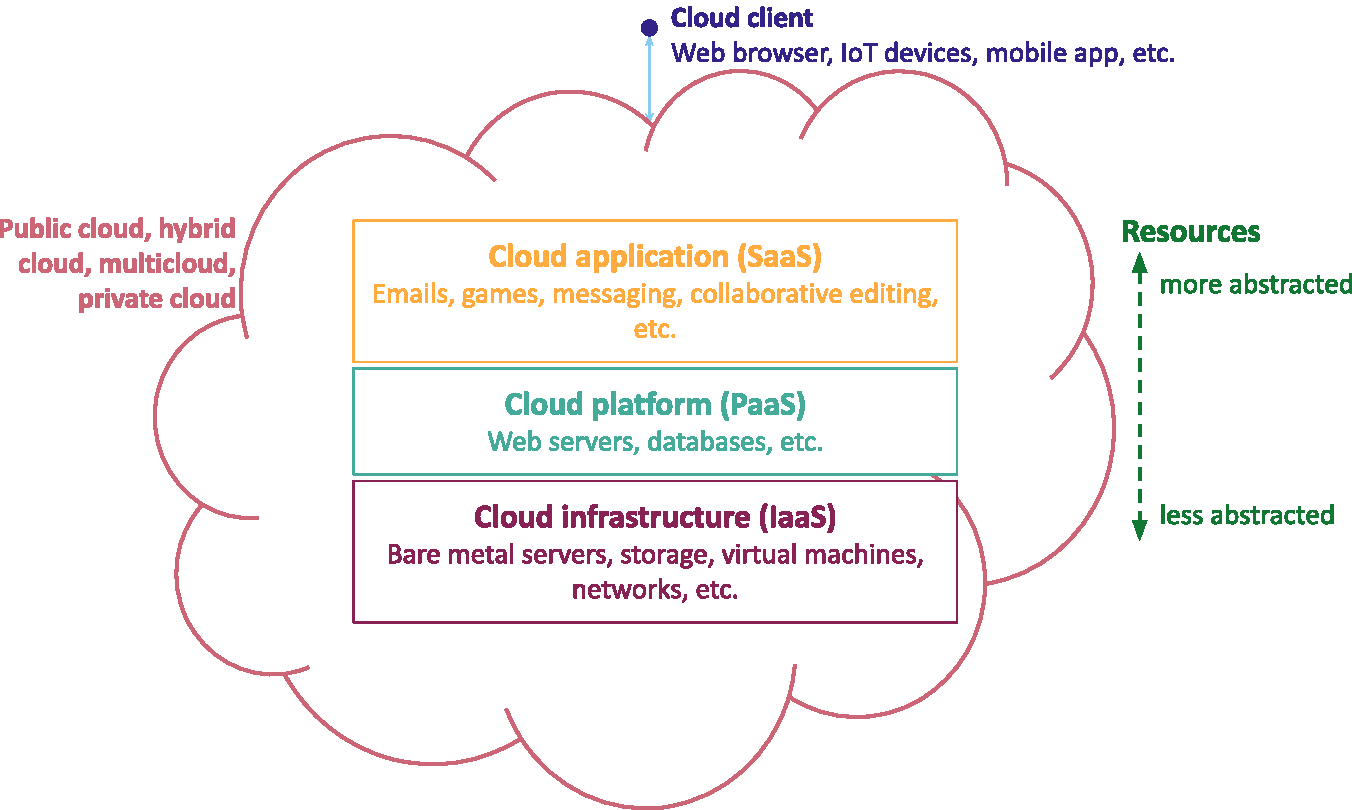
\includegraphics[width=.8\linewidth]{figs/pdf/CloudaaS}
  \caption{Different service models of the Cloud}
  \label{fig:cloudaas}
\end{figure}



To be more formal, the NIST (National Institute of Standards and
Technology) defined 5 principal characteristics for the Cloud
computing model~\cite{MG+11}:
\begin{description}
\item [On-demand self-service.] A user can interact with service
  providers without the need for a human, to get computing resources,
  such as storage, \glspl{server}, network. We will talk more about these
  resources in the next~\autoref{ssec:cloud-infra}.
\item [Broad network access.] These resources are delivered through
  the Internet network and can be accessed from heterogeneous devices
  (mobile phone, laptop, etc.).
\item [Resource pooling.] Cloud computing resources are pooled to
  serve multiple users at the same time (this is called multi-tenancy),
  and can be dynamically assigned depending on demand. Usually, the
  users have neither control nor knowledge of the exact location of
  the resources they are served. Sometimes, they may be able to
  specify the global location (such as country, region, \gls{dc}).
\item [Rapid elasticity.] Resources can be dynamically provisioned,
  used and released to scale up or down automatically per user
  demand. They often can appear virtually unlimited to the users.
\item [Measured service.] The resources usage is monitored, which
  allows to optimize it. This usage can be measured, controlled and
  described to provide transparency for both the users and the provider.
\end{description}


% A really important takeout from this overview of the Cloud is that
% resources managed by applications \emph{of} the Cloud are really
% diverse, from VMs to IPs, from email to text.


\subsection{Cloud Infrastructures}
\label{ssec:cloud-infra}

% To dive more into what a Cloud application is, we have to understand
% what are the characteristics of datacenters.

Whether we are speaking of large \dcs or smaller, on premises, sets of
hardware components, Cloud infrastructures building blocks are usually
collocated and as homogeneous as possible. This is the hardware layer.

An abstraction layer virtualizing resources is often used to bring a
better infrastructure logic to allow network and system administrators
to manage these infrastructures more easily. This is the
infrastructure layer that can be directly offered as a service (IaaS,
as seen in~\autoref{ssec:cloud-overview}). Then come platform and
applications layers (PaaS and SaaS).

Hardware, storage, network and virtualization compose the Cloud
infrastructure.
\begin{description}
\item[Hardware] includes \glspl{server}, as can one expect, but also
  \gls{disk array}s, network components such as \glspl{router},
  \gls{switch}es, etc.
\item[Virtualization] is the component that links physical hardware
  from abstracted layers. Typically, a \gls{hypervisor} abstracts the
  underlying hardware resources to link them logically and make them
  more easy to manage as pools of global resources in the
  infrastructure.
\item[Storage] is managed to back up data automatically or manually,
  ensure that older backups are automatically removed when they are no
  longer relevant, etc. It abstracts the physical storage through
  virtualization to offer Cloud storage solutions.
\item[Network] is composed of the physical network components on which
  virtual networks are created. Typically, virtual networks have
  different virtual resources that can be used, such as static/dynamic
  IPs, private or public sub-networks.
\end{description}

All the virtualized resources, including the network resources, are
pooled as usable entities ``independently'' of the physical resources
under, which means a user can exploit for example storage from two
different parts of the same \dc without even realizing it, as it was
one single entity.



\section{Cloud applications}
\label{sec:cloud-app}

Cloud applications, also called Cloud-native applications because they
were developed specifically for the Cloud, are the software that users
can access to execute services remotely, in \emph{the Cloud}.
%
More specifically, these applications run on top of two systems:
client-side (for example, the users' computer, or their browser) and
server-side (which is contacted by the application on the
client-side).


There are a lot of types of Cloud applications. But for most of them,
they are a set of independent, \gls{loosely coupled}, small \glspl{service},
connected with each other to form an entire, functional application.

In the rest of this thesis manuscript, we will use indiscriminately
\gls{microservice}~\cite{Tho15} or service to define these services
that are used to decouple functionalities in Cloud applications.
%
It is important to define also here that though we talked about
infrastructure computing resources before, from now on, we will use
the word \emph{resource} alone (unless it is obvious we talk about
infrastructure resources) to describe values that can be manipulated
by an application, and some can be stored in a data store, but it is
not mandatory. These resources can also have side effects when
manipulated.


\begin{figure}[htbp]
  \centering
  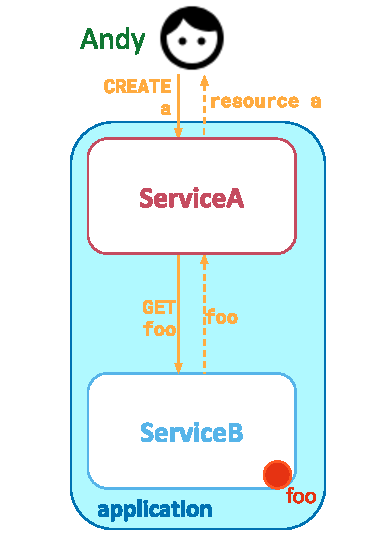
\includegraphics[width=0.3\textwidth]{figs/pdf/application}
  \caption{A typical Cloud application}
  \label{fig:typical-app}
\end{figure}

\autoref{fig:typical-app} presents a typical \gls{microservice} based Cloud
application.
%
The blue rectangle around represents the entire Cloud application.
%
A user (Andy), asks to \verb|CREATE| a resource \verb|a|.
%
The calls are shown in \textbf{{\color{CbOrange}orange}}, full arrows
; the responses in \textbf{{\color{CbOrange}orange}}, dashed
arrows.
%
\textbf{{\color{CbRose}ServiceA}} represents the service called by
Andy, which requires a sub-resource \verb|foo| from
\textbf{{\color{CbCyan}ServiceB}}, to create the requested resource
$a$.
%
Notice that \verb|ServiceA| effectively requests (\verb|GET|)
automatically, by itself, the sub-resource \verb|foo| from
\verb|ServiceB|, without any more intervention from the user.

In a more practical example for this figure, imagine that Andy wants
to create an account on an e-commerce website.
%
\verb|ServiceA| could be the service which creates and manages
accounts, and \verb|ServiceB| a service which creates and manages a
randomly generated image as an avatar for the account.
%
Andy asks an account creation, and \verb|ServiceA| will execute this request,
getting a random image from \verb|ServiceB| to create the account.
%
In this case, resource \verb|a| would consist in different information on
the account, and \verb|foo| the image.


% \todofig{Cloud application with a user using tikz}

% \begin{figure}[htbp]
%     \centering
%     \scalebox{.9}{%
%     \begin{tikzpicture}
%       \node[labeled] (App) {$App$};
%       \service[right=of App.north, matrix anchor=north west]{s}{e,f}
%       \service[right=of s]{t}{g,h}

%       % Workflow
%       \draw [->] (s-2-1) -- (t-3-1);

%       \node (c) [left=12mm of s-2-1] {$\bullet$};
%       \draw [->] (c)      edge (s-2-1.west);
%     \end{tikzpicture}
%     }
%     \caption{Application $App$ made of two services $s$ and $t$ and
%       four endpoints $e, f, g, h$. The $s.e \rightarrow t.h$
%       represents an example of a workflow.}
%     \label{fig:application}
%   \caption{Microservices architecture of a Cloud application}
%   \label{fig:soa}
% \end{figure}



% \section{Manage Cloud infrastructures} % 2p
% \label{sec:cloud-infra}

\section{Conclusion on the Cloud}
\label{sec:cccloud}

The Cloud is composed of hardware and software capabilities offered to
users, who do not have to manage the underlying infrastructure or even
have the compute capabilities.
%
Users only require a device to connect to \emph{the Cloud} thanks to
the device they do have to get the resources they need to complete
their tasks.

%
This comes with benefits such as scalability and flexibility of Cloud
resources, availability of the offered services without having to own
and maintain the required hardware.
%
The Cloud is usually physically located in public or private data
centers, that can be really huge and are typically not really close to
the users, but rather placed where costs for the infrastructure are low.

Cloud applications, running in the Cloud, are the ones that will be
manipulated by users to achieve their goals in the Cloud, and are
often composed of services that fulfill one functionality of the
application and are connected together to achieve the entire
application purpose.

We will now discuss what is the Edge computing paradigm, which comes
from the Cloud computing one.


\chapter{What is the Edge?} % 10p
\label{chap:edge}

In this Chapter, we are going to see what is the Edge and how it
differs from the Cloud.
%
Then, we will discuss what are the challenges of running an
application at the Edge, shedding more light on why it is difficult.

\section{Definition and purpose} % 6p
\label{sec:edge-def}

\subsection{Overview of the Edge}

The Edge is more recent and consisted originally in \glspl{Contentdn}
(\acrshort{CDN}), which \gls{cache}d and delivered large web content
such as videos~\cite{DPW04}. Since then, the technology evolved to deliver more than
static content~\cite{NSS10}.


The best way to envision the Edge as we consider it is to bring the
Cloud (computation and storage) closer to the users.
%
There are a lot of different views on what is the Edge, and how to
define it.%

%
Sometimes called Fog Computing, the part we are interested in is
located in between the Cloud \dcs and small devices that will collect
data or just need some computation to be done~\cite{SPDSM21}.
%
Some people only refer to the Edge as the devices that comprises the
closest devices from the users, and Fog for the layer between this
Edge and the Cloud~\cite{WVMN17}, or Fog as the continuum between Edge
and Cloud~\cite{MWTDV19}, or they use \glspl{cloudlet} as
Fog~\cite{SBCD09}.
%
We refer to those as Edge devices (or sensors and controllers), and
the \glspl{server} were the computation will mostly take place as Edge
\glspl{server}, or Edge \glspl{dc}, or for one set of collocated
\glspl{server}, as an Edge site.
%
Whatever the name, the \emph{Edge \glspl{dc}} will be the ones to
make the hard work, considering the devices at the Edge of the network
won't be able to carry it out, and will only collect data, sometimes
pre-process them\cite{SGDR21, TSS21, WFGI+19}, and in some case, even
those Edge sites will only do some parts, and the bulk of the tasks
will be executed in the Cloud.
%
% In some particular cases such as collaborative (or coordinated)
% applications where users collaborate for some tasks, such as
% \href{https://workspace.google.com/}{Google Doc}, the bulk of the workload will still be done on Edge devices


\begin{figure}
  \centering
  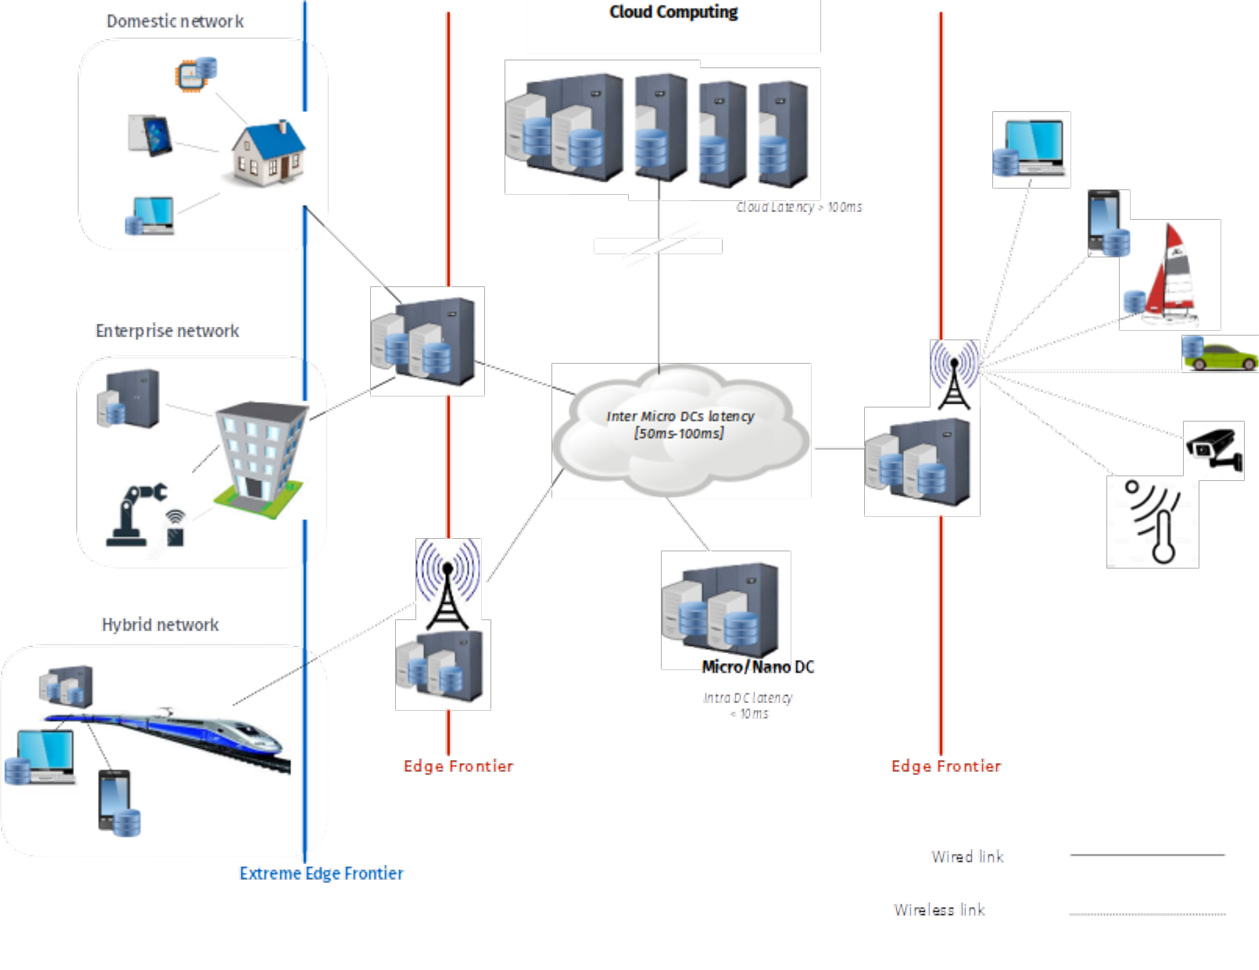
\includegraphics[width=0.8\textwidth]{figs/pdf/edge-infra}
  \caption{An overview of the Cloud and Edge (Source: \href{https://www.usenix.org/sites/default/files/conference/protected-files/hotedge18_slides_cherrueau.pdf}{Usenix - HotEdge'18})}
  \label{fig:edge-infra}
\end{figure}


The \emph{Edge \glspl{dc}} we are considering are thus in charge of
delivering Cloud capabilities to an Edge location (\ie a region, a
city, an business, an airport, etc.) and are composed of up to one
hundred \glspl{server}~\cite{CDL21}.
%
\autoref{fig:edge-infra} presents a view of Cloud \dcs and our
micro/nano-\dcs we discuss about.
%
They can be located anywhere, near the Edge devices, or in
\acrshort{PoP}s, on the Edge frontier.
%
We consider that the latency from clients to the Edge \dcs should be
around or less than 10ms, when the one to Cloud \dcs is between 50 to
100ms (or even more in worse cases, such as 150ms from Paris to Los
Angeles~\cite{pings}).

It is really important to understand that Cloud and Edge are
fundamentally the same in terms of the logic of offering resources,
storage, computing capabilities.
%
One way to see it is: imagine a really small \gls{dc}, and there
are thousands of them, distributed all around the globe.
%



\subsection{Intent}

The most obvious purpose of Edge computing is to improve (lower) the
latency between the location where a request is made and the place
where it is executed.
%
Indeed, since the distance is shorter between them, it is expected
that the response time will improve, on condition that the request is
executed as quickly on an Edge location as it will be further away in
the Cloud.

%
But by executing requests closer to the users, it is also expected to
save a lot of bandwidth on the parts of the network between \emph{the
  Cloud} (Cloud infrastructures) and the Edge.
%
This implies a reduction in data transfer costs.


%
Another potential benefit is to try and use renewable energy to run
the Edge infrastructures, by using farther sites when the closest
location energy is not sufficient to cover the execution of
requests~\cite{LYDP+18}, therefore increasing the sustainability of
the Edge computing~\cite{VLDH+21}.


To explicit the aim of the Edge computing, it is better to state some
of its potential applications.
%
As mentioned, the main purpose of the Edge is to reduce the response
time of \emph{Cloud requests} and execute the requests closer to where
they were made.
%
The Internet of Things (\acrshort{IoT}) is the most common example, with
the need for scalability, and avoiding flooding the usual network with
a lot of data.

\begin{figure}
  \centering
  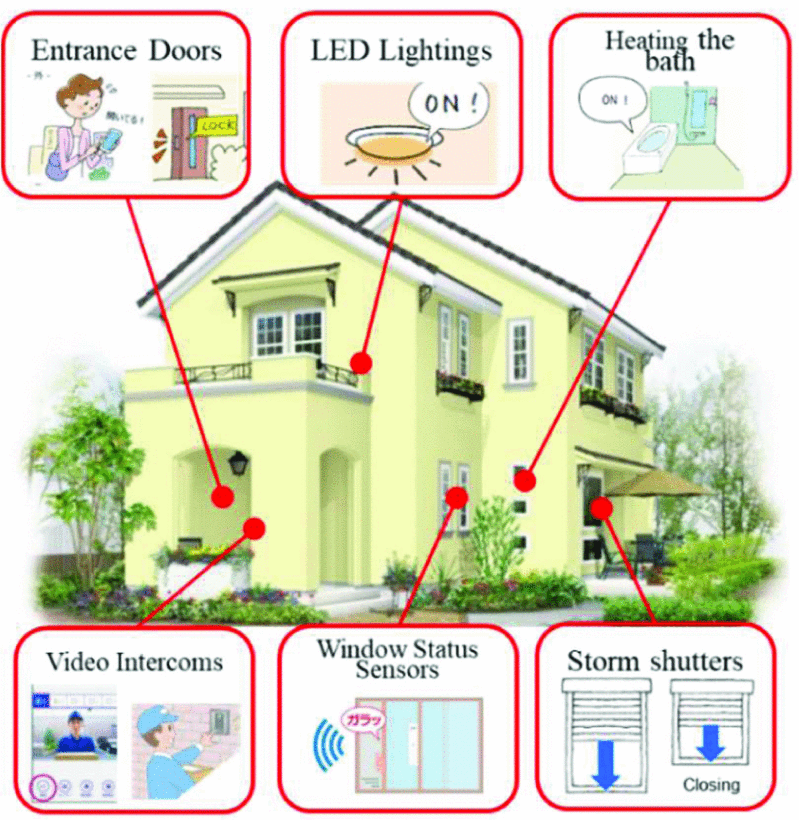
\includegraphics[width=0.6\textwidth]{figs/png/smart-homes}
  \caption{Overview of The Smart Homes from~\cite{II20}© 2020 IEEE}
  \label{fig:smart-home}
\end{figure}

And in particular, to give more concrete examples, Edge computing can
be used, among other use cases, in agriculture, \eg to improve
yield~\cite{SKPJ+19, DC19, JGE17}; in the oil industry, \eg to monitor
the transportation of the oil, for example~\cite{ALSL21, AONOA21}, in
a house, \eg to improve daily life or reduce energy costs~\cite{VBT16,
SH20, II20} or for smart cities~\cite{SKH18, YXCW+15}.
%
\autoref{fig:smart-home} shows examples on how to improve daily life
with smart homes, such as to control via application or automatically
through sensors different appliances in a house.





\section{Hostility of the Edge} % 2p
\label{sec:edge-chal}


% \section{What are the requirements for an application in such a context} % 2p
% \label{sec:edge-req}


Though the Edge can be really powerful to avoid use of bandwidth (by
going more local) and gives a lower latency for the applications
requiring it, there are also some challenges that come with it.

It is a hostile and challenging environment~\cite{MZCBT22, VWBKN16}
for Cloud applications, with \textbf{latency} that come through the
roof when different locations on opposite sides of the globe need to
communicate with each other: the user is indeed closer to one Edge
location, but maybe its request demands a resource that is far away
and will need to be fetched.
%
Moreover, overload can be generated on the network or in the
overall application because of the scale and stability of the system
can highly increase response time~\cite{platform9-latency, SCZKX16}.


Another challenge to be considered is the \textbf{heterogeneity} of
resources on which the applications will run~\cite{HoBl19}.
%
In our case, we do not really consider the Edge devices (\eg
\acrshort{IoT}), but even with small \dcs around the globe, it
implies that probably different actors will be involved.
%
And with different actors, or even often when we consider a single
actor, the infrastructure (hardware, protocols and Operating Systems)
of each site will probably differ from another~\cite{XJLC+19, SCZKX16}.

The \textbf{scale} of the infrastructure is also another
challenge~\cite{edge-challenges, mirantis-edge-challenges}.
%
Having small \glspl{dc} around the globe close to the user
implicitly says that there are going to be a lot of them; and that
the applications running on it need to be highly scalable.


Alongside the two last challenges comes the difficulties of control
and management of those sites, or put differently, the
\textbf{operational constraints}~\cite{edge-challenges, SCZKX16}.
%
First, how to ensure the reliance of the equipment, network, and more
generally the infrastructure environment in such a geo-distributed and
at high scale.
%
Second, how to have a global view of the entire infrastructure
made from so much a large number of site and heterogeneous hardware.
%
And third, how to ensure the security on this infrastructure,
especially how to isolate workload while having a global view.


%
But probably the worst aspect of Edge computing is that
\textbf{disconnections} between Edge locations are the norm rather
than the exception~\cite{SR21, IRPCM22}.
%
This is a huge problem when considering pushing Cloud applications to
the Edge.
%
Cloud applications assume a high reliance of the
infrastructure~\cite{Tamiru21}, so having parts of the pooled
resources from the Edge infrastructure unavailable suddenly is
definitely an issue~\cite{JS20}.

\section{Conclusion on the Edge} % 2p
\label{sec:ccedge}

The Edge computing paradigm has been created to deal with more and
more devices and applications requiring a low latency for the request
they were making to the Cloud.

As several different definitions exist for the Edge, I need to
reiterate here that in this manuscript, we refer as Edge, small
\glspl{dc} (up to a hundred servers), located near the users (less or
around than 10ms latency), that will serve either as the main point of
request executions, or as a relay for small requests, and redirect the
larger requests to the Cloud.

There are a lot of applications for the Edge, but it comes with some
inherent problems to tackle, such as heterogeneity, scale,
operational constraints, and most important, \textbf{frequent
disconnections} and the \textbf{latency} between different sites.

With these specifics in mind, we will now take an interest in how to
put Cloud applications at the Edge.


\chapter{Bringing Cloud applications to the Edge} % 5p
\label{chap:cloud-app-to-edge}



In this chapter, we state the principles and requirements identified
in this thesis as necessary to bring existing Cloud applications to
the Edge considering the challenges mentioned in the previous chapter.


% \section{Which type of Cloud Applications are we talking about}
% \label{sec:app-def}

% why
The main point of this thesis is about bringing existing, functioning
Cloud Applications to the Edge.
%
Since some of these applications are huge, to push these applications
from Cloud to Edge, we want to avoid changing their code as much as
possible.
%
%
These applications had some assumptions about the underlying
infrastructure it would be deployed upon.
%
These assumptions no longer make sense in the Edge context, with
failures and disconnections happening regularly all over the
infrastructure, as was just mentioned in the previous chapter.




\section{Defining principles and expectations}
\label{sec:principles}


In order to deal with the specific challenges stated
in~\autoref{sec:edge-chal}, applications in Edge computing have to
manage the geo-distribution of resources themselves~\cite{TBRT19}.


In~\cite{ST17}, the authors describe a distributed system as:
\begin{quote}
  A distributed system is a collection of autonomous computing
  elements that appears to its users as a single coherent system.
\end{quote}

In a geographically distributed environment, we need to follow two
major principles we introduced in~\cite{CDL21}:

\begin{description}
\item [Local-first]:~Minimize communications between sites and be able
to deal with network partitioning issues by continuing to serve local
requests at least.
 \item [Collaborative-then]:~Be able to take advantage of the
 different sites according to users' needs and infrastructure
 considerations.
\end{description}

The local-first principle has also been defined for \emph{local-first
software} in~\cite{local-first}; with seven ideals that should come
with it: fast, multi-device, ability to function offline,
collaboration between users, longevity, privacy, and user ownership
and control.
%
Moreover, for some applications such as social applications, the
propagation of the content is often localized, so a lot of processing
can be executed close to the point of origin~\cite{WLSY12}.

%
A lot of Cloud applications were created not as monoliths, but by
separating the code into collections of functionalities that apply one
resource or a small set of resources, called services~\cite{JPM+18,
Fie00}, as mentioned in~\autoref{sec:cloud-app}.
%
Some approaches to use Cloud applications at the Edge use this to
deploy different services/functionalities on different sites, or
different instances of the same service on different \glspl{server} or
sites, for balancing purposes~\cite{WVMN17,ROCW14,FLR16} .

From my point of view, the easiest way to ensure the local-first
principle is by having an entire instance of the application on each
site, which coincides with the description of distributed systems
above (autonomous computing elements).
%
%
But autonomous instances alone do not provide a way to ensure the
\emph{collaborative-then} principle.
%
In order to share diverse resources and enhance the capabilities of
the geo-distributed cloud application, an instance on one site should
be able to collaborate with other instances on other sites if need
be~\cite{BJ13}.

With the collaborations between all the instances of every sites, we
can get a single coherent system.
%
This view of a single coherent system I am aiming at and described in
the definition of a distributed system, is also comparable to the
Single System Image (SSI), which is composed of physical or logical
mechanisms to give the illusion that a set of distributed,
heterogeneous resources (hardware) forms a unique and shared computing
resource~\cite{BCJ01}.

With those principles, we can have a geo-distributed application
running at the Edge.
%
But these principles are not enough to specifically bring Cloud
applications to the Edge, with its inherent constraints.
%
Thus, several requirements I deem necessary in this context of
bringing Cloud applications to the Edge follow, with some of them
joining the local-first software ideals.


\begin{description}
\item [Non-intrusive:] One thing we do not want to do is change the
code of the application to geo-distribute it.
%
This is not mandatory for the Edge, but since it is a gain in time, it
is one of the roots of my approach.
%
The main reason is that some Cloud applications are huge and thus
changing their code is tedious and afterwards difficult to maintain.
\item [Generic:] This is not a requirement for the Edge per-say, but
  in order to be largely used, the bulk of the effort to push an
  existing application to the Edge should be (almost) ready to be used
  by developers for their applications, with a minimum production from
  their parts to plug to the solution if necessary.
\item [Tolerance to network partition:] This is the criteria of being
robust to network partition.
%
Since the Edge infrastructure is globally distributed, an application
deployed at the Edge must reckon with the challenges coming with a
wide-area network~\cite{LCR17}, one of them being frequent
disconnections and network partition.
%
It is different from the local-first principle because this is not the
only way to envision tolerance to network partition, such as
replication and distribution of services.
\item [Dynamic placement of requests execution:] The location of
requests execution should be handled dynamically.
%and as much as possible, not statically in a configuration file.
%
In the context of the Edge, it is important that requests can be
executed dynamically as the Edge itself is pretty
dynamic~\cite{FYWCS22}, with nodes connecting and disconnecting often.
%
By default, a static service composition establishes the collaboration
between services inside one instance permanently~\cite{DS05}.
%
It presents great advantages for the developer.
%
Modularity and static composition anticipates the services interface,
behavior and location.
%
Therefore, it guarantees the correctness of services’ invocations and
proper execution of the application~\cite{CJ01}.
%

In \os, for instance, the compute service is configured, once and for
all, to always request the image service in the same DC.
%
Hence, the compute does not mess with an unacquainted service.
%
However, these guarantees comes with the cost of an unyielding
application~\cite{DS05,FS04} that prevents on-the-fly collaborations.
\item [On-demand execution location:] The
location of execution of requests should be chosen per request by the
users of the application for several reasons~\cite{TPTE21}.
%

First, the need for privacy and trust is really important in the
context of the Cloud, and equally important in the Edge.
%
To ensure that the users privacy is respected, it is always easier to
let them choose where their resources will be located and manipulated,
which sites they trust.
%

Second, to avoid overloading each node with resources, it is
appropriate to have public resources scattered across the
infrastructure and usable at will, only when needed.
%
In this regard, it is intimately linked to the collaborative-then
principle.
%

This requirement is crucial, because it is always possible to add a
layer on top that would choose the location of requests execution
either by learning where the users usually execute their requests or
depending on nodes availability and/or latency, or using the
information on the nodes uptime for reliability~\cite{FMPS10, Lim21}.
%
This layer could be added if the need arose to avoid lengthy and
redundant information in requests or if a more transparent definition
is required, \eg for simplicity.
%
But it would be more difficult to give the users the choice of
defining their needs finely, on-demand, rather than automatize everything
from the beginning.
\item [Decentralized:] In the goal of coping with the network faults,
a centralized approach means some of the logic of the application will
not be able to be executed in case of a disconnection (it is a Single
Point of Failure).
%

A centralized approach is also a bottleneck, as all requests that need
to be handled by a central authority will need to go through the same
site, and goes against the goal of lowered latency of the Edge, as
requests will need to go further most of the time (breaking our
local-first principle as well).
\item [\Gls{p2p} (\acrshort{P2P}):] This properties derives from other
aforementioned requirements (local-first, tolerance to network
partitions, decentralized), but adds the necessity for equally
privileged instances of the applications; and it goes along by default
with having autonomous instances of an application everywhere.
%
Moreover, as the main challenges of the Edge are frequent
disconnections, latency and distributed resources between nodes of the
infrastructure, it makes sense to check if the adopted solution can be
considered as \acrshort{P2P} approach as these are the challenges that a
\gls{p2p} system deals with automatically~\cite{Sch01}.
\end{description}




\section{Premises of solutions} % 3p
\label{sec:c-to-e-solutions}



While the local-first principle can be ensured single-handedly by
having an entire instance of an application on each site, it
automatically prevents the use of resources between the sites if the
application was not designed for this.
%

Thus, with such a deployment, we have isolated applications that only
work with their own resources and we do not leverage the overall Edge
infrastructure.
%
Moreover, sharing resources between those different instances makes
sense in the context of the Edge, where the mobility of the users and
the locality of execution is crucial~\cite{SCZKX16, CLPW+18}.
%
Accessing a resource that is on another instance of the application
requires additional pieces of code that is not really dedicated to the
application business, and worse, that only has this particular
function.
%
% Moreover, the challenges of data management in distributed systems
% alone are good reasons to keep this need separated from the
% rest~\cite{Bloom}.

A way to share resources between multiple instances of an application
is to leverage both the service composition and the fact that multiple
instances of an application share the same services, that thus expose
the same \gls{api} (\acrshort{API}).
%
This is simple inter-service communication (ISC) that goes from one
site to another, as it can be used for load-balancing purposes.
%
Unfortunately, though this type of collaboration is easy to realize,
it does not provide a global view that would be expected as one
single, coherent system.

To achieve this view, such as a SSI we mentioned in the
previous~\autoref{sec:principles}, we need to be able to manage
resources between different instances of the same service.
%
To allow this, each service must be extended with some code that
allows more collaboration.
%
We refer to this type of collaboration as intra-service collaboration,
because it is used within the logic of one service, between multiple
instances of the same service.
%
The problem that goes with this dedicated code is that it goes beyond
the initial purpose of the service and thus includes collaboration
code in the business code of the service.
%
Although this dedicated means can benefit from message passing
middlewares or distributed databases internally, it always requires
invasive and complex code~\cite{CDLR+20}.
%
This is a well-known, challenging, and error-prone task for developers
of the application~\cite{ACHM11, BHJL+87, HR85}, who prefer not to
take resource sharing into account most of the time.
%
But the other side is that these sorts of collaborations allow a
global vision of resources managed by the applications, because
users are thus be able to retrieve any resource from anywhere in the
system/infrastructure.


\begin{figure}[htbp]
  \centering
  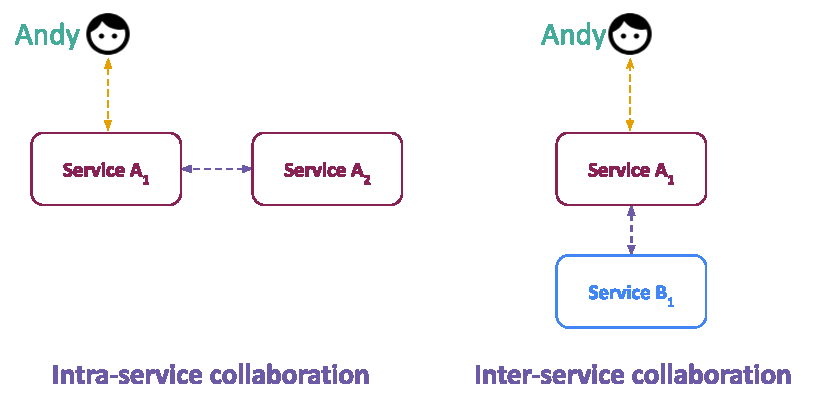
\includegraphics[width=0.8\textwidth]{figs/pdf/collaborations}
  \caption{Intra and inter-service collaborations}
  \label{fig:intera-collabs}
\end{figure}

So we have two types of collaborations between services: intra and
inter.
%
The former implements the collaborations of different instances
of the same service; the latter the collaborations between different
services and, in our case, especially from different services across
application instances or sites.
%
Both types of collaborations are presented
in~\autoref{fig:intera-collabs}.
%
In \textbf{intra-service collaborations}, we can see that the user interacts
with one service, and there is \emph{some kind} of collaboration
between the two instances of the same service to fulfill the request.
%
For example, getting some information from whichever database the
other instance of the service is connected to (assuming they are not
connected to the same database, as they would on two different
autonomous sites).
%
In \textbf{inter-service collaborations}, the
collaboration is made between two different services.
%
In two different instances of an application, it could be possible to
execute this collaboration between two different instances of two
different services.
% such as the case of having one entire application deployed on each
% site,   .
%
Both those types of collaborations ensure a single coherent
system that leverages the entire infrastructure and every resources
available.
%


\section{Why current solutions do not fit all our expectations} % 2p
\label{sec:why-no}

% In the previous section, we discussed how to have a single system view
% with autonomous instances of an application, we need intra and
% inter collaborations.

To allow these types of collaborations, while having a single coherent
system, three types of solutions exist in the litterature.


\begin{figure}[htbp]
  \centering
  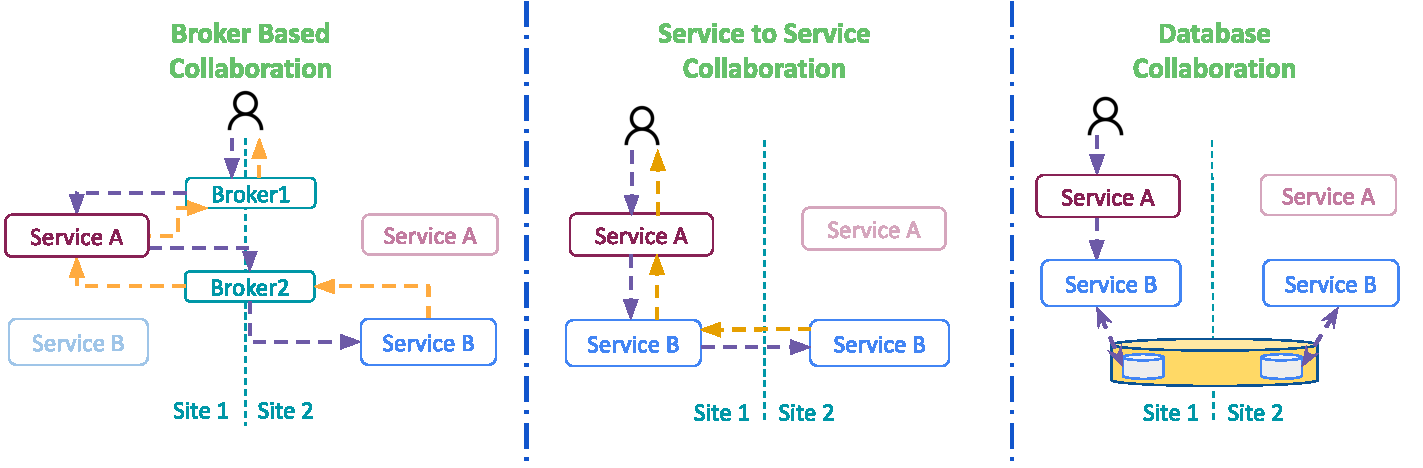
\includegraphics[width=1\textwidth]{figs/pdf/solutions}
  \caption{Different types of solutions}
  \label{fig:edge-solutions}
\end{figure}

\autoref{fig:edge-solutions} presents these three approaches.
%
The first is a broker based solution, which allows for inter-service
collaborations.
%
The broker approach allows externalization of collaboration aspects
away from the business code.
%
However, this approach requires a lot of development effort for an
application.
%
In addition to requiring a broker stub for each service, each broker
should implement once again a lot of what the original functionalities
of the service (because the broker needs to offer the same
capabilities as the underlying service in a geo-distributed and
transparent manner).
%
The alternative is having a generic broker to all services and
applications, which is difficult to envision because of the
differences between them.

Another interesting approach is service-to-service collaborations,
which is an intra-service collaboration.
%
As discussed before, this type of collaboration requires dedicated
code in the service, which is not related to its core logic.

Finally, the third approach is the one we explored previously to this
PhD~\cite{LPSD17, Che17, DCL18}, using databases or data stores, as
the current accepted research direction for developing geo-distributed
applications consists in using globally distributed data
stores~\cite{Aba12}.
%
Distributed data stores emulate a shared memory space among the
different instances of the application to make the development of
geo-distributed application easier~\cite{SBPB+18}.

%
I will now present more thoroughly this approach, as we discovered by
using it why the inherent problems to adopt it for an existing Cloud
application.

%One of the ways to allow


% \autoref{fig:edge-solutions} presents different solutions that are
% available to bring Cloud-native applications to the Edge.



\subsection{In particular: the issue of geo-distributing \os with a distributed data store}
\label{ssec:issue-db}


Most of this part comes from our Euro-Par paper~\cite{CDL21}, and is
also discussed in our Research Report from 2020~\cite{CDLR+20}, both
written with Ronan-Alexandre Cherrueau and Adrien Lebre, and the
second also with Javier Rojas Balderrama and Matthieu Simonin.
%
To explain the issues with this approach, I will use \os as an
example, since it is by trying to use it at this Edge we identified
these issues, and previous studies based on a shared database already
paved the way for \os~\cite{LPSD17, BPC16}.
%
OpenStack is a resource management application to operate one DC.  It
is responsible for booting Virtual Machines (VMs), assigning VMs in
networks, storing operating system images, administrating users, or
any operation related to the management of a DC.
%
It is thus both an Cloud application and an application to manage
Clouds.
%
It is a good example of what we want to geo-distribute, as \os is
around 13M lines of code~\cite{openstackloc}, so a huge application we
do not want to change.


\subsubsection{A complex but modular application.}

Similarly to other Cloud applications, \os follows a modular design
with many services.
%
It has been developed to run natively on one single \gls{dc}.
%
Some efforts have been made along its development to make it run on
multiple clusters, even at large scale.
%
For example, some involved to allow service-to-service collaboration
for specific services (like Keystone~\cite{keystonefed},
Glance~\cite{glance-edge}), but it requires a lot of efforts for all
services to add the features and to maintain them.
%
The compute service for example manages the compute resources of a
\acrshort{DC} to boot VMs.
%
The image service controls operating system \acrshort{blob}s like Debian.
\autoref{fig:os} depicts this modular design in the context of a boot
of a VM.
%
The user starts by addressing a boot request to the compute
service of the DC (Step 1).
%
\begin{figure}[h]
  \centering
  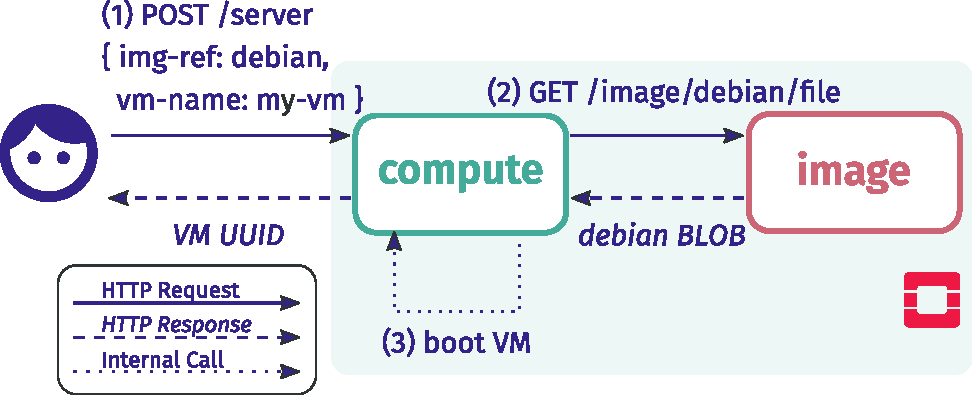
\includegraphics[width=.7\linewidth]{figs/pdf/openstack-vmprovision}
  \caption{Boot of a Debian VM in OpenStack}
  \label{fig:os}
\end{figure}
%
The compute service handles the request and contacts the image service
to get the Debian blob in return (Step 2).
%
Finally, the compute does a bunch of internal calls, such as schedule
VM, setup the network, mount the drive with the blob, before booting
the new VM onto one of its compute nodes (Step 3)\footnote{For
clarity, the boot workflow is simplified here. In a real OpenStack
deployment, the boot also requires at least the network and identity
service. Many other service may also be involved.  See
\url{https://www.openstack.org/software/}.  Accessed 2022-10-02}


\subsubsection{Geo-distributing Openstack.}

Following the local-first and collaborative-then principles implies
two important considerations for OpenStack.
%
First, each DC should behave like a usual cloud infrastructure where
users can make requests and use resources belonging to one site
without any external communication to other sites.
%
Second, users should be able to manipulate resources between DCs if
needed~\cite{CLPW+18}.
%
For instance, \autoref{fig:os-share} illustrates an hypothetical
sharing with the ``boot of a VM at one DC using the Debian image
available in a second one'' scenario.
%
\begin{figure}[h]
  \centering
  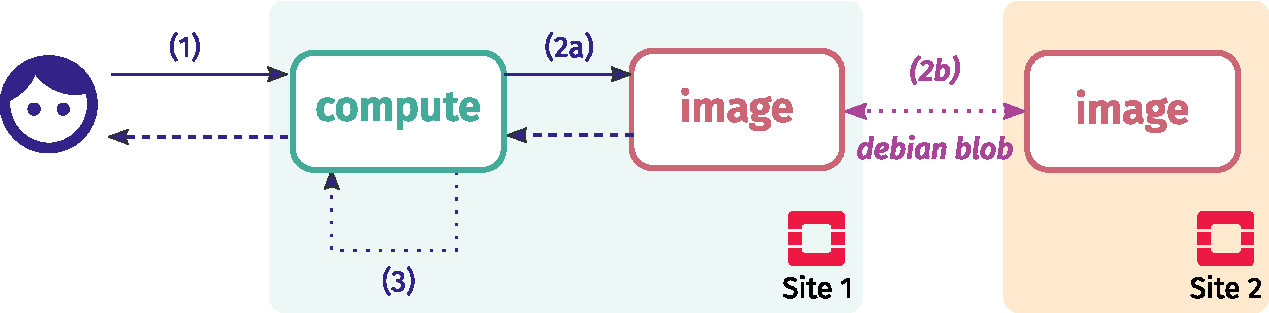
\includegraphics[width=.8\linewidth]{figs/pdf/openstack-share}
  \caption{Boot of a VM using a remote blob}
  \label{fig:os-share}
\end{figure}

To provide this resource sharing between \sOne and \sTwo, the image
service has to implement an additional dedicated means (Step 2b).
%
Moreover, it should be configurable as it might be relevant to
replicate the resource if the sharing is supposed to be done multiple
times over a WAN link.
%
Implementing such a mechanism is a tedious task for programmers of the
application, who might prefer to rely on a distributed data
store~\cite{CDEF+12}.


\subsubsection{Problem: distributed data store tangles the geo-distribution concern.}
\label{ssec:pb1}

The OpenStack image service team studied several solutions to
implement the ``booting a VM at \sOne that benefits from images in
\sTwo'' scenario.
%
All are based on a distributed data store that provides resource
sharing between multiple image services: a pull mode where \sOne
instance gets blobs from \sTwo using a message passing middleware, a
system that replicates blobs around instances using a shared database,
etc.~\cite{glance-edge}
%
The bottom line is that they all require to \emph{entangle} the
geo-distribution concern within the logic of the application.
%
This can be illustrated by the code that retrieves a blob when a
request is issued on the image service (code at Step~2 from
\autoref{fig:os-share}).


\begin{lstlisting}[
    caption={Retrieval of a blob in the image service},
    label=lst:glance,
    numbers=left,
    frame=lines,
    float=tb,
    basicstyle=\footnotesize,
    ]
@app.get('/image/{name}/file')
def get_image(name: String) -> blob:
  # Lookup the image path in the data store:
  # `path = proto://path/debian.qcow`
  path = ds.query(f'''SELECT path FROM images WHERE id IS "{name}";''')

  # Read path to get the image blob
  image_blob = image_collection.get(path)
  return image_blob
\end{lstlisting}

\autoref{lst:glance} gives a coarse-grained description of that code.
%
It first queries the data store to find the path of the blob (l.~5).
%
It then retrieves that blob in the \verb|image_collection| and returns
it to the caller using the \verb|get| method (l.~6--8).
%
Particularly, this method resolves the protocol of the \verb/path/ and
calls the proper library to get the image.
%
Most of the time, that path refers to a blob address on the local disk
(\eg \verb|file:///path/debian.qcow|).
%
In such a case, the method \verb|image_collection.get| relies on the
local \verb|open| python function to get the blob.

\begin{figure}[h]
  \centering
  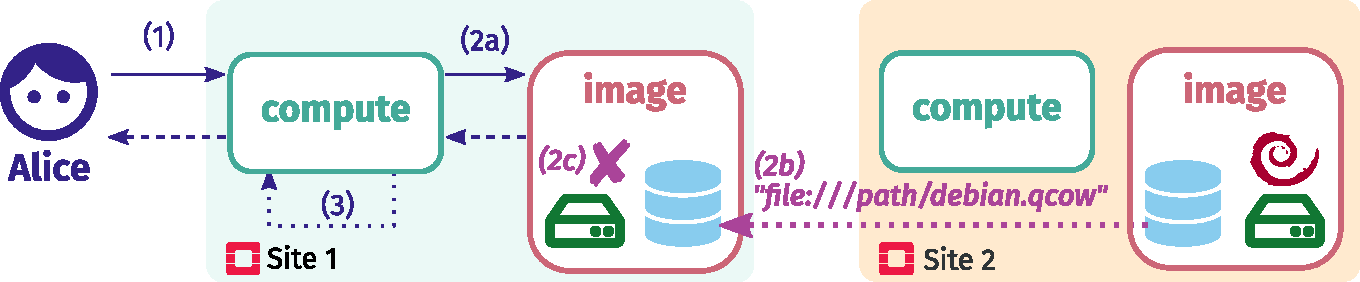
\includegraphics[width=1\linewidth]{figs/pdf/openstack-db-backend}
  \caption{Booting a VM at \sOne with a blob in \sTwo using a
    distributed data store (does not work)}
  \label{fig:glance}
\end{figure}

%
The code executes properly as long as only one OpenStack is involved.
%
But things go wrong when multiple are unified through a data store.
%
\autoref{fig:glance} presents how it is a problem.
%
If \autoref{lst:glance} remains unchanged, then the sole difference in
the workflow of ``booting a VM at \sOne using an image in \sTwo'' is
the distributed data store that federates all image paths (including
those in \sTwo).
%
Unfortunately, because \sTwo hosts the Debian image, the file path of
that image returned at Step 2b is local to \sTwo and \emph{does not
exist} on the disk of \sOne.
%
An \emph{error} results in the \verb|image_collection.get| (2c).

The execution of the method \verb|image_collection.get| takes place in
a specific environment called its \emph{execution context}.
%
This context contains explicit data such as the method parameters.
%
In our case, the image \verb|path| found from the data store.
%
It also contains implicit assumptions made by the programmer: ``A path
with the \verb|file:| prototype must refer to an image stored on the
local disk''.
%
Alas, such kind of assumptions are wrong with a distributed data
store.
%
The code has to be fixed.
%
For this scenario of ``booting a VM at \sOne using an image in
\sTwo'', it means changing the \verb|image_collection.get| method in
order to allow the access of the disk of \sTwo from \sOne.
%
More generally, a distributed data store constrains programmers to
take the distribution into account (and the struggle to achieved it)
in the application.
%
And besides this entanglement, a distributed data store also strongly
limits the collaborative-then principle.
%
In the code above, there is no way to specify whether a particular
blob should be replicated or not, for example.
%

The geo-distribution thus must be handled outside of the business
logic and in a fine-grained manner due to its complexity, along with
the requirements stated before.


\section{Conclusion on the context} % 2p
\label{sec:cccontext}

As we discussed throughout this part (\autoref{p:context}), Cloud
applications were not designed to face the Edge challenges, especially
the disconnections and latency problems inherent to this paradigm.

As we want to bring Cloud appplications to the Edge, and considering
that some are huge, we want to avoid changing their original code as
much as possible and find a generic solution that can be used for a
lot of applications.

This is why I defined these principles for a possible solution:
  \begin{itemize}
  \item \textbf{local-first} to work autonomously
  \item \textbf{collaborative-then} to leverage the infrastructure
  \item \textbf{non-intrusive} regarding the code of the application
  \item \textbf{generic} to a lot of existing applications
  \item \textbf{tolerance to network partition} for the Edge
    disconnections problems
  \item \textbf{dynamic placement} of requests to cope with the
    dynamism of the Edge infrastructure
  \item placement \textbf{decided by the users}, per request, when
    needed
  \item \textbf{decentralized} to avoid single points of failure
    complications
  \item \textbf{P2P} to match the aforementioned principles:
    local-first, tolerance to network partitions, decentralized
  \end{itemize}

  As I was defining the principles required for the solution I want to
  answer my research question of bringing Cloud applications to the
  Edge, I specified the logic of a solution for the collaborations
  between different instances of the exact same application deployed
  on each location while keeping a single coherent system.

  We have overviewed why different solutions for collaborations,
  namely \emph{non-generic brokers},
  \emph{service-to-service}/federation, and \emph{distributed
    databases}, are not generic and imply to code the collaborations
  for each service (broker, service-to-service), or entangle
  non-business information into the code (database), which
  automatically goes against the non-intrusive principle.

  In the next part (\autoref{p:soa}), we will observe how the
  state-of-the-art solutions envision their own different ways to
  bring Cloud applications to the Edge, as well as taking a peek on
  how Edge applications can be developed to check if we can learn
  ideas on how to build this bridge between the two computing
  paradigms.


\clearemptydoublepage

\part[State of the Art]{Using applications at the Edge: a state of the art}
\label{p:soa}

\epigraph{We got tactical smart missiles, phased plasma pulse rifles, RPGs, we got sonic electronic ball breakers! We got nukes, we got knives, sharp sticks...}{Private Hudson, Aliens}


\begin{comment}
* Using applications at the Edge: a state of the art - 45p
** Developing an application for the Edge - 20p
** Managing the Edge infrastructure - 20p
** Using Cloud Applications at the Edge - 5p
\end{comment}

In this part, we will compare academic and industry approaches
to put an application at the Edge.
%
We have seen in the previous part (\autoref{sec:why-no}) how
approaches to deal with the collaborations to provide a single
coherent system are not satisfying.
%
Now, we will investigate how other approaches can be made without
necessarily having to deal with the collaborations, by pushing
applications to the Edge in different manners.
%based on the requirements we defined in~\autoref{sec:principles}.

The goal of this part is mainly to study interesting solutions in the
literature to first, obviously, avoid reinventing the wheel.
%
This will be ensured by the comparison of our requirements to these
approaches; if they fit my requirements, it is not necessary to make
it from scratch.
%
Second, even if some requirements are not enforced, parts of the
approaches can be interesting to build my own approach, and thus
answer the questions raised.
%
Finally, it can be useful to give insights of functioning ideas that
do not fit our requirements to be able to question them.


Because I wanted my solution to be generic to a lot of Cloud
applications, there is a broad spectrum of approaches that can be of
interest to us.
%
As a smaller goal, I tried to focus on the most interesting approaches
regarding our requirements and/or the representativity of the solution
for each section.

First, I present in~\autoref{chap:comparison} the comparison points
based on the requirements we defined in~\autoref{sec:principles}.
%

%
\autoref{chap:soa-edge-infra} presents ways to manage the Edge
infrastructure so we can deploy applications on it.
%
In particular, \autoref{chap:soa-SM} presents service meshes for the
Cloud to explore the possibility of using them at the Edge.
%

Then, I present in~\autoref{chap:soa-dev-edge-app} how it is possible
to make Edge-native applications.
%
%

Finally,~\autoref{chap:soa-conclusion} concludes on the overall
comparison on papers.


\chapter{Comparison points}
\label{chap:comparison}

This chapter presents the different categories on which I will
compare different approaches.

Because the comparison points are not entirely binary, the path I
chose to compare the solutions is to attribute clouds (\cloud), from
one to three.
%
As a disclaimer, I tried to define the attribution of clouds as
decisive as possible, but for some categories it is difficult to be
unquestionable and some attributions might seem to be unfair for a
specific approach.
%
It is important to note that this comparison is not a grading
operation and a difference from one cloud in the attribution does not
really matter because we are not saying that an approach is better
than another, but simply I am comparing them to my requirements.
%
\textbf{If the category is entirely out of scope for a specific
  solution, such as if it was not considered at all, no clouds will be
  attributed}.
%
I will now present, for each category, how I will attribute clouds.


\begin{description}
\item [Non-intrusive (NF)] As mentioned, one thing we do not want to
  do is change the code of the application to geo-distribute a Cloud
  application.
  %

  Three clouds correspond to no touching at all; two clouds if the
  approach needed to change some of the vanilla code, and one cloud
  for touching the coding without changing its fundamental logic.
\item [Generic] For our solution, we chose to be as generic as
  possible.
  %

  Three clouds are given for approaches that would function on a large
  set of applications; two clouds when it is generic for applications
  that would be able to run on top of the approach (if it is available
  for Kubernetes-based solutions for example); and one cloud if it is
  only functioning for applications from the same development team,
  that share for example the same specific \acrshort{API}.
\item [Local-first (LF)] The local-first principle, explained in
  ~\autoref{sec:principles}, correspond to the ability of the solution
  to use at minimum the local site to serve requests in case of a
  network partition.
  %

  Three clouds were attributed if the application is entirely
  available locally; two if most of it is available at all time (\eg
  an effort has been put for the most common requests); and one cloud
  if at least some part of the business logic is available on any
  site.
\item [Collaborative-then (CT)] Autonomous instances of an application
  should be able to collaborate to leverage the entire infrastructure
  and resources.
  %

  Three clouds are given for approaches that allow different sites to
  collaborate for any kind of resources; two when it is only a subset
  of resources; one when only some resources can be shared.
\item [Network partition (NP)] This is the criteria of being robust to
  network partition.
  %
  It is separated from the local-first principle because this is not
  the only way to envision tolerance to network partition.
  %

  Three clouds are awarded for solutions that allows sites to work
  autonomously and/or merge the changes as required after; two clouds
  if resources are available in a read-only mode or in other way to
  get them and one cloud if network partition is tolerated only if
  another site is cut from the network or only in some specific cases.
\item [Dynamic] The location of execution of requests should be
  handled dynamically and not statically in a configuration file.
  %

  Three clouds are given for an approach in which the location is
  selected dynamically; two clouds if the information of sites
  locations is given in a configuration file but used dynamically
  afterwards and I did not find in the literature any approach that
  would define or justify one cloud, so no ``one cloud'' will be
  attributed on this point.
\item [On-demand] The location of execution of requests should be
  chosen per request by the users of the application for different
  reasons mentioned in~\autoref{sec:principles}.
  %

  Three clouds were granted if users can choose requests execution
  location at fine grain while building their requests; two clouds if
  the user can define this location per request, one if they need to
  define the location globally and/or statically (and thus, also not
  dynamic), or if they do not chose the location, but is is decided by
  the application.
\item [Decentralized] The approach we envision must be decentralized
  to avoid losing some to all functionalities of the application.
  %
  Usually, approaches that are not fully decentralized will not
  fulfill the local-first principle and thus, typically cannot be
  tolerant to network partitions.

  %
  Three clouds were given for decentralized approaches; two if the
  approach is partially decentralized, but leverage the Edge-to-Cloud
  continuum to execute only some part of the workload in the Cloud;
  and one cloud if the main part of the application is centralized in
  the Cloud and the Edge only execute the rest.

\item [Peer-to Peer (P2P)] This is about equality of privileges on the
  different sites of the infrastructures.
  %

  Three clouds were given if all instances of the applications have
  the same privileges.
  %
  Two if all the sites are equals but some sites are more \emph{equal}
  than others, as George Orwell would have put it (\ie if some sites
  do not have the exact same privileges as others).
  %
  One cloud for approaches where most of the decisions are made on a
  few nodes and the bulk of the nodes are mostly producers/workers.
\end{description}

For every solution we will observe in this part, I will give an
overview of the approach, the clouds attributed for each of these
points of comparison and a short conclusion on the solution, with
information on what was relevant exactly for me.




\chapter{Managing Edge applications on Edge infrastructures}
\label{chap:soa-edge-infra}

In this part, we will focus on ways to leverage an Edge or
Cloud/Edge infrastructure with virtualized resources on which we
can deploy applications.
%
To understand the importance of checking what was done for managing
the Edge infrastructure, it is crucial to grasp these two points: (i)
in the Cloud, infrastructure are managed by Cloud applications
(offering \acrshort{iaas}), (ii) if we can push these Cloud
applications to the Edge themselves, we would have Edge infrastructure
managers that can be used to deploy applications following our
requirements.

As our main goal is to push Cloud applications to the Edge, having
management applications for the Edge \emph{for free} is definitely
worth investigating.

We will first investigate specifically applications able to
orchestrate services, and after, we will see more general approaches.



\section{Orchestration}
\label{sec:orchestration}


Cloud Orchestration applications have the ability to automatically
configure, coordinate and manage a Cloud system.
%
They manage the life-cycle of services and provide users with the
required services for their workload.
%
They also monitor the infrastructure and services to adapt the system
according to the requirements~\cite{DP06}.

\cite{CBCA23} is a survey on Fog orchestration, which corresponds
mostly to what we define as Edge.
%
The authors determined that among the main goals of the orchestration
in the studied literature, resource management is the most cited,
followed by guarantee of Service Level Agreements (what standards of
services will be offered) and service life cycle management.
%
Both services and applications are the most orchestrated entities
(respectively in 36\% and 34\% of the studied literature), followed by
tasks.
%
The topology of the approaches in their corpus was mostly
\emph{centralized}, some were \emph{decentralized} (with some
hierarchy), and only a few were \emph{distributed} (no central or
leader node).


One of the most common ways to orchestrate the Cloud is to use
(containers) orchestration, especially with Kubernetes, even for the
Fog or Edge context~\cite{TPTE21, UVK21, UDAD+21, WSMB18, BGCCV19,
  SZPDC17}.
%
In~\cite{GTV19}, the authors define three requirements for container
orchestration for Edge nodes in the Edge-to-Cloud continuum:

\begin{itemize}
\item compatibility with modern container standards, or provision of
  an equivalent
\item securitization of the communications between the layers of the
  Cloud and the Edge nodes.
\item low resource requirements to be run on Edge nodes
\end{itemize}
These requirements allowed them to create a lightweight container
orchestrator called FLEDGE.

In fact, there are a lot of different approaches~\cite{BW22}, both in
the academic world and in the industry, with some still in use or
being developed.
%
Manaouil et al.\cite{ML20} presents how three approaches to revise
Kubernetes original code to better deal with the geo-distribution, \ie
Kubefed~\cite{kubefed} and Submariner~\cite{submariner}, which do not
deliver the illusion of a single Kubernetes system and
KubeEdge~\cite{XSXH18, kubeedge}, which is not decentralized, as it is
the case for one of the solution for \os, StarlingX~\cite{starlingx}.
%
And in any of these cases, the goal was to change the vanilla code of
Kubernetes, which we do not want.

We will now present other relevant approaches.

% \subsection{Collaborative Cloud - Edge: A Declarative API
% orchestration model for the NextGen 5G Core~\cite{UVK21}}
% \label{subsec:UVK21}

% \subsection{EdgeX over Kubernetes~\cite{LPPKK21}}
% \label{subsec:LPPKK21}

% \subsection{Container Orchestration Techniques in Cloud and Edge/Fog Computing Environments~\cite{WB21}}
% \label{subsec:WB21}

% There is also Krossboard and SuperEdge, but not detailed enough

\subsection{Decentralized and Fault Tolerant Cloud Service
  Orchestration~\cite{Spataru20}}
\label{subsec:spataru20}

This paper from Spataru presents an approached to decentralize the
CloudLightning project, a framework to orchestrate Cloud Services with
the goal to use it upon Edge resources owned by individuals or even
small-scale clusters.
%
Though the Edge is not mentioned in this paper, the project call the
resources at the Edge \emph{heterogeneous Cloud} and they mention the
Fog Computing, which also corresponds to what we, in this thesis, call
Edge Computing.

In CloudLightning, there are two different components, namely
\emph{Gateway Service} and \emph{Resource Manager} which use physical
resources thanks to an hypervisor.
%
The Gateway Service maintains a catalog of services, described in
TOSCA (Topology and Orchestration Specification for Cloud
Applications, which has been extended specifically for Fog and Edge
deployments~\cite{TVCAM21}), to compose an application.
%
Users send a description of their requirements and abstract services
to form an application and the \emph{Service Optimization Engine} in
the Gateway Service choose the best implementation (topology) among
the catalog and depending on the availability of the system.
%
Afterwards, the orchestrator reads the topology and deploys it, after
which it will monitor the deployment and execution of the involved
services, restarting them in case of failure.
%
In the Resource manager, there is a service to ``Plug\&Play'' the
hypervisor which could deploy VMs or containers, and the hypervisor is
registered in the Self Organizing Self Managing (SOSM) system.
%
There is also a telemetry service which stores data from a telemetry
client which has to be connected to this system.
%
Finally, bare metal servers can also be used through configuration.

The SOSM system is self-healing and aggregates monitoring information
to assess the performance of the computation resources depending on
the business objectives. It keeps a suitability index to guide the
requests towards better resources.

\begin{figure}[htbp]
  \centering  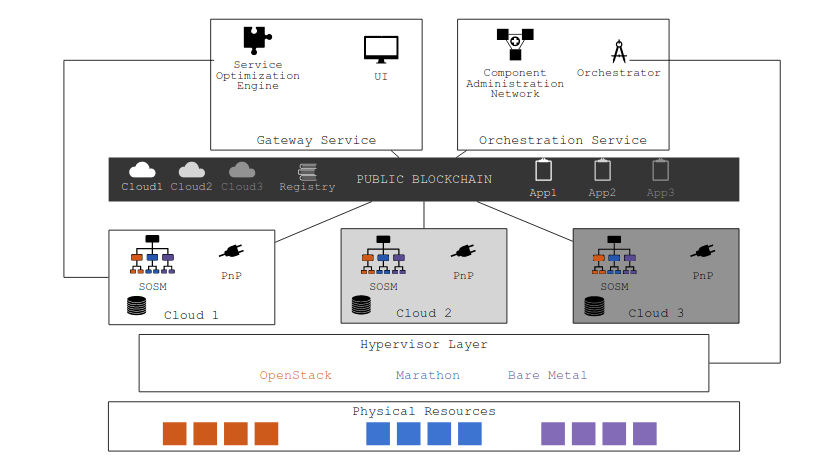
\includegraphics[width=1\linewidth]{figs/png/decentralizedcloudlightning}
  \caption{Augmented Decentralized CloudLightning Architecture}
  \label{fig:decent-cl}
\end{figure}


When a service fails, as mentioned, the Orchestrator will restart it
and the services depending on it will need to have the endpoints
updated to be able to keep communications.

There is a capability of decentralizing CloudLightning components,
which will be able to be discovered through \glspl{smart contract} on
a public blockchain.
%
This augmented architecture is presented in~\autoref{fig:decent-cl},
with the decentralized components:
\begin{itemize}
\item the registry contract keeps information on Cloud Providers,
  Services and Applications
\item the cloud contract keeps resources description (as well as their
  prices) and endpoints for the scheduler and Plug\&Play components
\item the application contract tracks deployment status and payments
\end{itemize}

Finally, the paper presents the Component Administration Networks
which make the link between Smart Contracts and Software components,
as well as giving monitoring and fault-tolerance capabilities to sets
of replicas.
%
This component is composed of three layers.
%
The first one is the underlying \acrshort{P2P} network of nodes that
collaborate and maintain the Ethereum blockchain.
%
The second layer manages the nodes thanks to a leader of the network,
that controls the transactions related to the component.
%
The third layer administer the components (such as (de)registration of
components, assign them some workload, etc.)


\subsubsection*{Comparison}

This approach is non-intrusive, using either VMs, containers or bare
metal, so it is also generic.

It does not follow the principle of local-first, as the services will
be separated depending on the best placement available, but those
services are allowed to collaborate through their configuration.

In case of a network partition, the services on the involved node will
probably be restarted elsewhere, but then the application on the
involved node will probably not be able to function as it would not
have all the services available.

Requests can be redirected to ``better'' computational resources
dynamically, but not on the user decision.
%
The users only define their requirements for the application.

This approach is fully decentralized and uses a blockchain to keep the
information on this decentralized approach.

% The authors use a blockchain and smart contracts for resource registration and assignment.


\subsubsection*{Conclusion}

In conclusion, this paper presents an enhance version of the
CloudLightning framework, to provide a decentralized orchestrator of
Cloud Services in the context of computing resources composed of home
computers or small-scale data centers.
%
The main goal of this paper is to pave the way for a decentralized
Cloud with individually owned resources serves as compute nodes, and
ways to deal with the payment of these resources.
%

The originality of this approach resides mainly on the use of a
blockchain and smart contracts to decentralize the control on the
orchestration.




\subsection{Liquid computing and Liqo~\cite{IRPCM22}}
\label{subsec:liqo}

Liqo is a solution to transparently manage different clusters in
Kubernetes, orchestrating them and allowing (computing) resource
sharing between those clusters.
%
The authors of the paper envision their approach, \emph{liquid
  computing}, as a continuum of resources and services to allow
transparent and infrastructure-agnostic deployment of applications.

For each workload, users can assign constraints such as geographical
locality, cost, capabilities, etc.
%
Their approach derives from a \acrshort{P2P} approach, with no centralized
control and no intrinsically privileged members.
%
Each actor (owner of a cluster) is the overall infrastructure keeps
the full control of their own infrastructure and decides how many
resources and services they share and with whom.
%
As in usual \acrshort{P2P} system, the topology is fluid and able to manage
dynamic changes, with frequent and sometimes unexpected connections
and disconnections.

It is built on different key concepts used for the liquid computing.
%
The first one is the discovery and peering functions. The peering in
their approach is a unidirectional resource and service consumption
relationship, which provides flexibility, but which can be combined to
support bidirectional peering.
%
Second, they distinguish nodes as local (attached to the consuming
cluster), virtual (abstracted and pooled resources) and big (for nodes
with much more capabilities than other average nodes), which allow
them to envision different types of clusters and a hierarchical
representation of the resources.
%
Third, to achieve robustness, tolerance to network disconnections and
scalability, they introduce the concept of resource reflection:
objects exist in their \emph{native} form in the local cluster and in
their \emph{shadow} form remotely.
%
Finally, the need for network, and storage and data continuum, where,
in the first one, the overlapping of different networks across the
cluster is a problem and should have a network fabric to handle
transparently this problem; and in the second one, the workload should
follow as much as possible its involved data.

Liqo itself is the project to enforce the liquid computing approach.
%
It extends -and is built upon- Kubernetes without any change in its
standard \acrshort{API}.

\subsubsection*{Comparison}

%
The approach is generic regarding the applications that will run in
the pods, but in itself, Liqo only works with Kubernetes solutions,
even though their key concepts could be applied to other orchestrator.
%

%
Each cluster works independently if need be, so it follows the rules
of local-first and collaborative-then, and thus a site can be used
during network partitions.

Liqo's approach needs some configurations to establish \acrshort{P2P},
but afterwards, the attribution of clusters is dynamic.
%
The location of execution of a request is chosen automatically per
scheduling, but \emph{intent-driven}, defined by users.
%, which means that the users can define a set of high-level policies
% to express associated constraints for the execution.

%
The goal of the approach is to offload pods on other sites by defining
unidirectional peering links, that can be combined to get a real
\acrshort{P2P} approach.

\subsubsection*{Conclusion}

The liquid computing concept and its associated project, Liqo aim at
envisioning a continuum of resources and services in a transparent and
infrastructure-agnostic manner.
%
The authors of the paper defined their vision, in which the main
characteristics are intent-driven definitions of the workloads,
decentralized architecture, multi-ownership and fluid topology.

From these principles, they deduce some pillars, key concepts, to allow
for the materialization of the liquid computing.
%
Finally, they present Liqo, their open-source project built on top of
Kubernetes to implement their vision through multi-cluster topologies.

Though this approach is really interesting in terms of our
requirements, the lack of user-defined requests at fined grain is
probably what is missing for the requirements.



\subsection{HYDRA: Decentralized Location-aware Orchestration of
  Containerized Applications~\cite{JS20}}
\label{subsec:JS20}

HYDRA~\cite{JS20} is a Proof of Concept (\acrshort{poc}) decentralized and
location-aware orchestrator that manages microservices in
containerized applications, written by Jimenez and Schelen.

In this paper, a focus is made on the location-aware version of the
orchestrator, even if it can run location-agnostic.
%
HYDRA builds a \acrshort{P2P} overlay network of nodes, where a node
is any hardware (virtualized or not) that can execute containerized
services, and thus a node is both orchestrator and (computing)
resource.
%
Four roles are available for the nodes:
\begin{itemize}
\item The entry role is temporary and corresponds to the role assumed
  when a node receive a request to deploy, remove or modify
  applications, where it needs to transfer this request to the
  appropriate nodes on the orchestrator network that will manage the
  request. The role is removed when the request has been served.
\item There are two controller roles, root and leaf, with the latter
  used only in location-aware control. The root controls the entire
  application, while the leaves manage only a set of services of the
  application.
\item The service host role is attributed to nodes who host and
  monitor services, and send heartbeats to the leader controller of
  those services for service liveness.
\end{itemize}

Depending on the number of required services, replicas of these
services, the need for scaling-out, and other considerations, the
number of service host nodes may change during the life-cycle of the
application.
%
These roles are not exclusive and a node can assume different roles
for different applications.

Users can deploy an application give its definition through a
\emph{recipe}, giving information on what and how to deploy, and how
it will be managed.
%
To deploy an application, the node in charge of deploying it launch
the search for viable nodes (in terms of resource availability with
the regards to the services requirements).
%
To find these nodes, the algorithm follows three properties:
\begin{itemize}
\item maximize the probability that the search will query different nodes
\item ensure that the load is spread across the HYDRA network evenly
\item leverage the information on the distance between nodes
\end{itemize}

Regarding the experiments, HYDRA is able to scale to at least 20 000
nodes, and support almost 30 000 applications running on 15 000 nodes.
%
The orchestrator nodes are able to work autonomously, and the location
awareness has almost no impact on the orchestrator performance.

\subsubsection*{Comparison}

Since it uses applications that run in containers, Hydra is non-intrusive
and generic to these existing Cloud applications.
%

The search for (computing) resources algorithm is randomized or use
new nodes as much as possible, so it is difficult to envision it is a
local-first approach.
%
Some services are deployed close to each other, but this is as local
as it gets.
%
On the other hand, it is a collaborative-then approach in the sense
that all resources can be used by any node.
%
The evaluation proves that the orchestrator itself still function in
case of network partitioning.
%

This approach can be considered dynamic because it requires a
configuration of the services, but then the requests are probably
routed depending on the application metadata, since some services are
replicated and so forth.
%
Because of that, the location is pre-defined from the users choice for
their applications, but afterwards, it is not chosen per-request.

The approach is designed to be fully decentralized, and all have nodes
can have the same privileges, even though they have different
privileges from the viewpoint of one application.


\subsubsection*{Conclusion}

HYDRA is a decentralized orchestrator for containerized microservices
based applications.
%
It allows for location-aware deployment and robust control of these
applications as well as management of heterogeneous Edge resources.
%
Finally, it provides resiliency of the deployed applications during
their life cycle.

This paper has many interesting approaches to solve problems that the
Edge can bring and follows a lot of our requirements.
%
Nonetheless, the location-awareness of the orchestrator does not allow
users to finely define the execution location of their request and it
lacks the requirement of local-first.


\section{Control planes and other managements}
\label{sec:other-management}

Some management tools do not fall into the orchestration category.
%
For example, \emph{control planes} are a layer in an application that will
manage higher functionalities such as monitoring, scaling, security,
configuration, etc. to make sure that the application runs properly
and as expected.
%
It is usually represented on top of the \emph{data plane}, which it controls,
as this one is the layer in charge of processing data requests, taking
orders from the control plane.

In this section, we will explore management solutions that can be seen
as these parts of the applications or just do not fit the
orchestration category.

\subsection{OneEdge: An Efficient Control Plane for Geo-Distributed
  Infrastructures~\cite{SGDR21}}
\label{subsec:SGDR21}

This paper from Saurez et al. presents a \emph{hybrid} control plane
for Edge infrastructures.
%
Like us, they consider infrastructures composed of different
micro-data centers, maintained by ISPs, with heterogeneous computation
resources.
%
They distinguish \emph{coordinated} applications which requires
collocation and coordination between different instances, such as
collaborative assisted driving and geo-distributed multiplayer games,
and \emph{standalone} applications which can work with a single
instance, such as virtual reality.
%
This approach is really interesting in the context of the Edge,
because it is easier to know where to put applications, depending on
these classes.
%
Some of the requirements they observed are also somehow close to ours:
\begin{description}
\item[Autonomous control] for latency-sensitive standalone
  applications, with single-site deployments
\item[Coordinated control] for coordinated applications, with
  multi-site deployments
\item[Spatial affinity] for applications location sensitivity
\item[End-to-end latency Service Level Objective] enforce the
  guarantees
\item[Dynamic resource allocation] for re-deployment in cases of
  mobility, failures, computing resource scarcity
\end{description}
Most of the differences have to do with the automated placement and
handling of users requests, and this is mainly were we have different
approaches.
%
In the context of the Edge (and more largely the Cloud), it is an
indubitably good idea and practice, but we chose to rely more on the
human intelligence and users and give them only information so they
can decide how to make their requests.

\subsubsection*{Comparison}

% no touching and genericity
OneEdge runs applications in containers and VMs, thus, without
changing their code. It is generic to existing Cloud
applications.

% Decentralization and \acrshort{P2P}
To coordinate applications instances, OneEdge has a centralized
controller to get a global view, but in order to keep autonomous,
rapid decisions without centralized coordination, an authoritative
state is kept on each site. The scheduling decisions are also left to
the Edge sites. Thus, most of the logic of the application is the same
everywhere, but not everything.


% LF CT
An effort has been made to decentralized the control plane as much as
possible, but keeping a central controller where decisions are made
(about placement and reallocation/migration through monitoring). The
collaborations between the sites are available for all types of
resources the control plane manages.

% NP
Most of the sites are autonomous, but for the centralized part, since
it is in the Cloud, fault tolerance is less important, but they ensure
it by having a secondary instance of the controller resubmitting the
requests (replicated on both instances) that have not be completed as
new requests. It is worth noting though, that the launch of
coordinated applications are forwarded to the central controller,
which is a problem in case of partitions.

% Dynamic OD
Users can request at any moment to launch an application, and these
requests are transferred to the closest site using a discovery
service. Thus, the control plane decide itself where a request will be
executed, but for each request, dynamically.


\subsubsection*{Conclusion}

OneEdge is a hybrid (in the sense of centralization) control plane
that allows some of the decision-making to be made autonomously on
Edge sites.
%
It presents an interesting approach to discriminate applications
between standalone and coordinated ones, which makes sense at the
Edge, because the needs are different.
%
To minimize deployment latency, standalone applications are scheduled
autonomously, while coordinated applications requires co-location and
thus, their deployment and scheduling is managed in a centralized
manner.
%
This hybrid approach of what can be done in a centralized manner or
not is a really interesting point that could be useful for other
approaches as it reduces the number of calls that will go to a
centralized \gls{dc}.
%
Nonetheless, it is not something I desired for my solution as I want a
decentralized and P2P approach.



\subsection{OpenYurt~\cite{openyurt}}
\label{subsec:oy}
OpenYurt is a platform extending Kubernetes to allow users to manage
large scale Edge computing workloads.
%
OpenYurt architecture is self-described like so:
\begin{quote}
  OpenYurt follows a classic cloud-edge architecture design. It uses a
  centralized Kubernetes control plane residing in the cloud site to
  manage multiple edge nodes residing in the edge sites. Each edge
  node has moderate compute resources available in order to run edge
  applications plus the required OpenYurt components. The edge nodes
  in a cluster can span multiple physical regions, which are referred
  to as Pools in OpenYurt.
\end{quote}

\autoref{fig:oy-arch} is the representation of OpenYurt architecture.
%
In this figure, the blue box represents the original Kubernetes
components, and the orange box the OpenYurt components.
%
This is a hierarchical approach in which Kubernetes \acrshort{API}
server is located in the Cloud, as well as OpenYurt Cloud node
management capabilities.
%
At the Edge part of the figure, the orange box represents what is
inside one node from any node pool on the right part.
%
Nodes at the Edge are composed of different Kubernetes
functionalities, such as Kubelet, KubeProxy, etc., and more
importantly of the pods themselves as well as OpenYurt Edge
functionalities.
%
For example, YurtHub serve as a sidecar to handle requests from
Kubernetes components on worker nodes and direct them to the
APIserver.
%
The connections from Edge nodes to the Cloud control plane is managed
by YurtTunnel (Server/Agent).


\begin{figure}[htbp]
  \centering  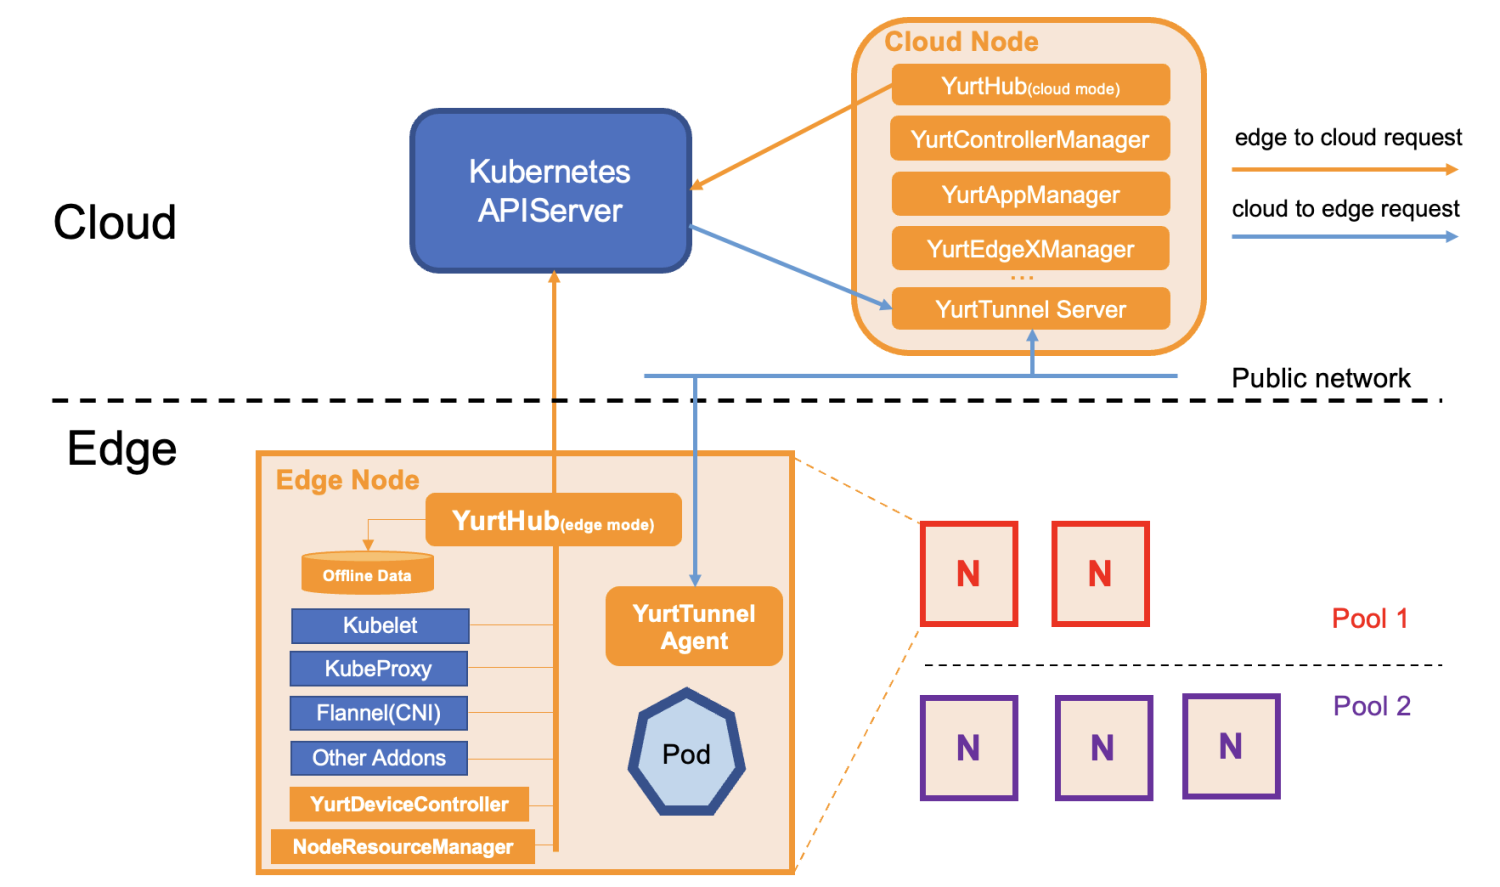
\includegraphics[width=.9\linewidth]{figs/png/openyurt-arch}
  \caption{OpenYurt architecture ( \href{https://github.com/openyurtio/openyurt}{Source: OpenYurt's Github}).}
  \label{fig:oy-arch}
\end{figure}

\subsubsection*{Comparison}

Using the original Kubernetes components, OpenYurt makes non-intrusive
enhancements, but the centralized control plane in the Cloud site
managing multiple Edge nodes makes it a not really \acrshort{P2P} approach.
%
It is generic to any application that can be run on Kubernetes.

%
Node autonomy is a functionality that allows Edge nodes to continue
running even though the Cloud-Edge link is severed, but it is only
available through configuration.
%
Moreover, node autonomy only means that users can manipulate existing
resources and not create new ones, so its partition tolerance is not
complete.

The collaboration are available for every resources managed by
Kubernetes.

%
It is worth mentioning that \emph{service topology} allows users to
decide to use in general the endpoints from the same node, or from the
same nodepool, so the general location execution of the request (by
general location policies) is decided globally by the users, and then
the application chose the exact location.

As it as a centralized control plane and a hierarchical architecture,
it is not decentralized and is not a \acrshort{P2P} system.

\subsubsection*{Conclusion}

OpenYurt is a self-described \emph{platform} that extends Kubernetes
to deliver a non-intrusive approach which can allow network partition
to some extent (\ie whatever does not need the control plane).
%
Regarding our requirements, it answers not entirely the local-first
and collaborative-then principles, as well as the network partition in
node autonomy mode.
%
Moreover, it lacks a decentralized approach and the ability for users
to make finely defined requests.



\subsection{Re-designing Cloud Platforms for Massive Scale using \acrshort{P2P}
  Architecture~\cite{SYHJ17}}
\label{subsec:SYHJ17}

In\cite{SYHJ17} (and~\cite{Han17}), Soares et al. present a way to use
\os on a large scale, using \acrshort{P2P} architecture.
%
Though it is not designed specifically for the Edge, scaling is the
first step towards a solution for the Edge, and the \acrshort{P2P} approach
checks some of our requirements.
%
They briefly introduce the concepts that were introduced in \os to
manage large scale deployments, such as Regions to manage the locality
of resources, or Availability zones which allows to logically
partition compute, storage or network resources, and finally Cells,
which allows to shard several compute resources into cells, and then
be dispatched in different locations.
%
But all these solutions had to be \emph{added} into \os code, and thus
are available whether you need them or not.

They follow three design principles:
\begin{itemize}
\item avoid centralized components as much as possible, for
  scalability and robustness purposes.
\item avoid as much as possible changes in the original code so it is
  easily adopted and can be more generic.
\item externalize problems to an existing outside system as much as
  possible to simplify the solution and minimize the efforts.
\end{itemize}

%
They deploy an entire instance of the Cloud management software on
every sites, calling the instance a \gls{cloudlet}.

%
On each site, they put their agent which can send a request to the
local \os or forward it to another site.
%
This agent implements a service proxy on each \os service.
%
Each proxy around a service expose the same \acrshort{API} as the
service they encapsulate, as well as request forwarding and
translation logic.
%
This follows the broker based collaboration presented
in~\autoref{sec:why-no}.
%
Each agent is also composed of an \emph{overlay management} which
allow the different agents to discover each other and identify which
agent sent a particular request.
%
Each agent has a \emph{state management} to allow them to keep
information about users and resources they own.
%
Finally, an interface allows the agents to communicate with each other
(Agent-to-Agent communication).

Each agent is responsible to handle every requests that come from any
user mapped with it.
%
This mapping is statically created when a user's tenant is created.
%
Through state management, each agent tracks the resources allocated to
a tenant, which is required to find resources that are not stored
locally but on other sites.
%
They keep they internal ID of the created resources and map them to
the cloudlet where the resource has been provisioned.
%
To improve robustness, this state information can be replicated on
several agents, but their implementation uses a simple database.

%
As a \acrshort{P2P} system, each site maintains a list of their
neighbors, where a transitive closure of the graph representing the
neighbor relationships returns all sites in the system.
%
More simply put, with every lists of the neighbors of every sites,
there is a complete view on the entire system.

Regarding specific services, they use the federated identity for
authentication and authorization, which is a service-to-service
functionality offered by \os.
%
For the image service, the image is found thanks to the mapping of
ID/site presented above.
%
For the scheduling/placement of VMs, they chose to balance the memory
load on all sites.
%
Finally, for the network, they do not use a specific approach but
mention it is a problem that is being addressed.
%
They mention the Tricircle approach~\cite{tricircle}, but since this
article is a bit dated, I would also like to mention this
approach~\cite{ELNC20}, which was one of the first steps for a part of
our own solution.


\subsubsection*{Comparison}

One of their design principles is to avoid touching the code as much
as possible, and in the paper, there is actually no mention of having
to change the code.
%
In their principles, they also mention that the external approach is
to make it generic, but no further fact is given about this, so we
consider it to be designed specifically for \os, even though it
probably can be adapted for this purpose.
%
In any case, since this approach manages a infrastructure manager, it
is generic to any application that could be run in an \os VM.

They operate an entire instance of \os on each cloudlet, so it works
perfectly locally on a standalone way.
%
It is collaborative through federation of some of the services and
through the agent for the rest.

The \acrshort{P2P} approach combined with the fact that there is an instance on
each site makes it tolerant to network partition.

The placement of the tenant is determined statically at its creation,
but otherwise, other requests are dynamic, following the list of
neighbors the agents know.
%
If some of the resource are treated locally as possible; the VMs,
which are somehow the principal resource of \os are automatically
placed, so we cannot really say it is per user request.

The approach is entirely decentralized and without hierarchical
management, designed as a \acrshort{P2P} system.



\subsubsection*{Conclusion}

This paper presents an approach to decentralize \os in a
non-intrusive and \acrshort{P2P} manner, with autonomous instances.

In this approach, images from Glance (the image service) are shared
across different sites.
%
They use internal IDs from their agent to keep tracks of these
resources shared on different sites with a mapping to IDs created by
\os to find the resources locally.
%
This is something really useful for our local-first and
collaborative-then principles and has actually been used in our
solution.

%
Since our initial focus was on \os, this paper was obviously
important in our early decision making, and especially before we
decided we needed a more generic and user-centric approach.



\section{Conclusion on managing applications on Edge infrastructure}
\label{sec:soa-em-conclusion}

To ease the reading of the table, we add the following reminder, for orchestration:
\begin{description}
\item [\cite{Spataru20}] Decentralized and Fault Tolerant Cloud Service Orchestration (\autoref{subsec:spataru20})
\item [\cite{IRPCM22}] Liquid computing and Liqo (\autoref{subsec:liqo})
\item [\cite{JS20}] HYDRA: Decentralized Location-aware Orchestration of Containerized Applications (\autoref{subsec:JS20})
\end{description}
And for control planes and other managements:
\begin{description}
\item [\cite{SGDR21}] OneEdge (\autoref{subsec:SGDR21})
\item [\cite{openyurt}] OpenYurt (\autoref{subsec:oy})
\item [\cite{SYHJ17}] Re-designing Cloud Platforms for Massive Scale using P2P Architecture (\autoref{subsec:SYHJ17})
\end{description}

\begin{table}[htbp]
  \centering
  \footnotesize\setlength{\tabcolsep}{4pt}
\begin{tabular}{|c|c|c|c|c|c|c|c|c|c|}
\hline
 & NI & generic & LF & CT & NP & dynamic & on-demand &  decentralized & P2P\\
\hline
  \cite{Spataru20} & \cloud \cloud \cloud  & \cloud \cloud \cloud  & - & \cloud \cloud \cloud  & \cloud  & \cloud \cloud \cloud  & \cloud  & \cloud \cloud \cloud  & \cloud \cloud \cloud \\
  \cite{IRPCM22} & \cloud \cloud \cloud  & \cloud \cloud  & \cloud \cloud \cloud  & \cloud \cloud \cloud  & \cloud \cloud \cloud  & \cloud \cloud  & \cloud \cloud  & \cloud \cloud \cloud  & \cloud \cloud \\
  \cite{JS20} & \cloud \cloud \cloud  & \cloud \cloud  & \cloud  & \cloud \cloud \cloud  & \cloud \cloud \cloud  & \cloud \cloud  & \cloud  & \cloud \cloud \cloud  & \cloud \cloud \cloud \\
  \hline
  \cite{SGDR21} & \cloud \cloud \cloud  & \cloud \cloud \cloud  & \cloud \cloud  & \cloud \cloud \cloud  & \cloud  & \cloud \cloud \cloud  & \cloud  & \cloud \cloud  & \cloud \cloud \\
  \cite{openyurt} & \cloud \cloud \cloud  & \cloud \cloud  & \cloud \cloud (1) & \cloud \cloud \cloud  & \cloud(1) & \cloud \cloud  & \cloud  & \cloud  & \cloud \\
  \cite{SYHJ17} & \cloud \cloud \cloud  & \cloud \cloud  & \cloud \cloud \cloud  & \cloud \cloud  & \cloud \cloud \cloud  & \cloud \cloud  & \cloud \cloud  & \cloud \cloud \cloud  & \cloud \cloud \cloud \\
  \hline
  \end{tabular}
  \caption{Comparison points on Edge infrastructure management.
    (1) Only available when activating node autonomy\protect\footnotemark.}
  \label{tab:soa-eim}
\end{table}


\footnotetext{\url{https://openyurt.io/docs/next/user-manuals/autonomy/node-autonomy}}

\autoref{tab:soa-eim} represents the comparison of the approaches to
orchestrate and manage Edge infrastructure to deploy applications.

The first part (the three first lines) are defined as orchestrators,
while the others are respectively identified as only a control plane,
a platform and an architecture for an existing management platform.

Whatever the name, they all can be used deploy workflow and
applications, via virtualization or containerization.

In terms of existing Cloud applications that are brought to the Edge,
\os is used in one of these approaches~\cite{SYHJ17}, while Kubernetes
is used in two of those approaches (\cite{IRPCM22, openyurt} and other
aforementioned approaches from the Orchestration introduction.
%
\cite{Spataru20} uses an existing project, CloudLightning as a base on
which to build upon.

The main requirement lacking in those approaches are the user-centric
decisions, but otherwise, some applications make solid candidate
regarding our base requirements introduced
in~\autoref{sec:principles}, such as~\cite{IRPCM22, openyurt},
though~\cite{openyurt} only offers tolerance to disconnections as a
\emph{degraded} mode.


Since none of the approaches corresponds entirely to my requirements,
we will now take interest in a way that could help to manage the
different instances of the application we want at the Edge, and
especially the collaborations between them.




\section{A service mesh at the Edge?}
\label{chap:soa-SM}

% Linkerd (one of the most used service mesh) defines a service mesh
% as~\cite{linkerd-sm}:
% \begin{quote}
%   A service mesh like Linkerd is a tool for adding observability,
%   security, and reliability features to “cloud native” applications by
%   transparently inserting this functionality at the platform layer
%   rather than the application layer. The service mesh is rapidly
%   becoming a standard part of the cloud native stack, especially for
%   Kubernetes adopters.
% \end{quote}

William Morgan from Buoyant Inc. (Buoyant created Linkerd, one of the
most used service mesh) defined services meshes as~\cite{LLGZG19}(© 2011 IEEE):

\begin{quote}
A service mesh is a dedicated infrastructure layer for handling
service-to-service communication. It’s responsible for the reliable
delivery of requests through the complex topology of services that
comprise a modern, cloud native application. In practice, the service
mesh is typically implemented as an array of lightweight network
proxies that are deployed alongside application code, without the
application needing to be aware.
\end{quote}

In practice, a service mesh helps with the separation of the tasks of
development from the operations.
%
The developers can focus on the business logic and code, and operators
on deploying the application, keeping it running, etc., as put by
William Morgan: [the service mesh is] ``deployed alongside application
code, without the application needing to be aware''.
%
Actually, RedHat specified that~\cite{redhat-sm}:
\begin{quote}
  Without a service mesh, each microservice needs to be coded with
  logic to govern service-to-service communication, which means
  developers are less focused on business goals.
\end{quote}
%
In this sense, a service mesh could help with the service
collaborations discussed in~\autoref{sec:c-to-e-solutions}.


It usually consists in a scalable set of proxies deployed with the
application~\cite{linkerd-sm}, as specified by William Morgan in the quote above.
%
These proxies, composing the \emph{data plane}, manage the
communications between the micro-services, passing them through the
\emph{control plane} to execute whichever functionalities the service
mesh provides.

\autoref{fig:sm-arch} presents an abstracted service mesh
architecture.
%
The control plane and the data plane are represented
separated.
%
Each service is deployed alongside a proxy as a sidecar,
but the proxy could also be represented as the capsule around the
service, because it intercepts incoming and outgoing communications to
transfer them to the control plane.
%
These proxies thus serve both as proxies and as reverse
proxies~\cite{rproxy}.
%
In the control plane, there are different components achieving the
functionalities of the service mesh, such as monitoring, service
discovery (to build a registry of services), etc.
%
Also, since it is an abstract representation, there can be any number
of services or components, which is shown as the dots on the right
part of the figure.

\begin{figure}[htbp]
  \centering  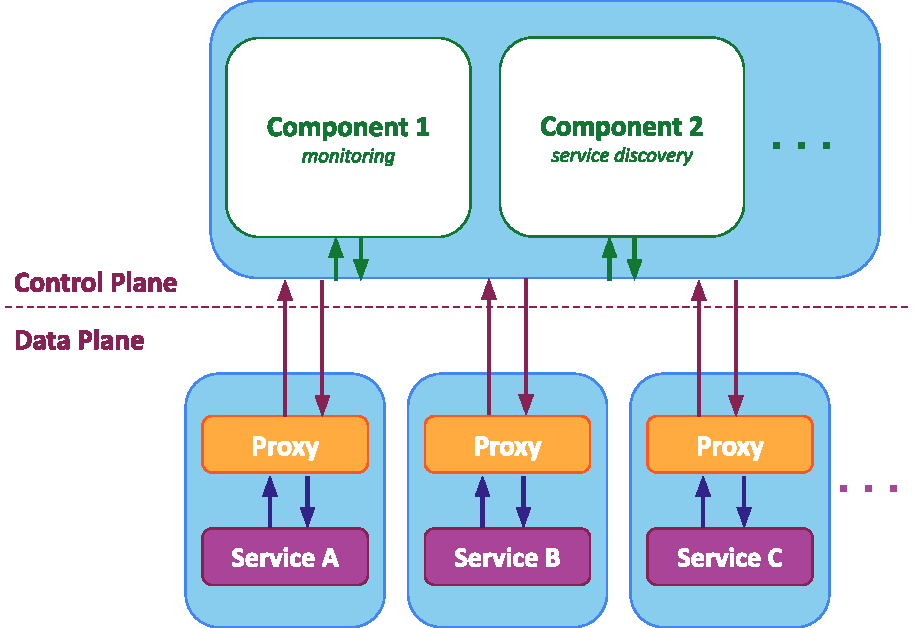
\includegraphics[width=0.75\linewidth]{figs/pdf/service-mesh}
  \caption{Architecture of a typical service mesh, inspired from \cite{SMmanifesto}}
  \label{fig:sm-arch}
\end{figure}


Though service meshes were not created in the first place for the
Edge, they are a very important software architectural framework for
Edge computing, because they could bring functionalities such as
service discovery, load-balancing, resiliency, scalability,
low-latency offloads and privacy~\cite{GRRL+21, LLGZG19}.



\subsection{Istio~\cite{SS20}}
\label{sec:soa-istio}

Istio is an open source service mesh that uses
Envoy\footnote{\url{https://www.envoyproxy.io/} - Accessed:
  2022-09-20} as the proxy.
%
Envoy is a proxy often used as a
dataplane\footnote{\url{https://servicemesh.es/} - Accessed:
  2022-09-20} and is deployed as a sidecar along each service.
%
Envoy has a L3, L4 and L7 filter layer, which allows to filter and
route \acrshort{TCP}/\acrshort{UDP}, \acrshort{TLS} (see \gls{tcp},
\gls{udp}, \gls{tls} for definitions), HTTP(/2) and \acrshort{gRPC}
requests, with much more functionality on the last two.


Istio provides traffic management through Envoy and service-level
properties (timeouts, retries, etc.) configurations, through the Istio
Pilot agent running in the sidecar or the gateway container.
%
The control plane also provides observability through the tracking of
requests, which allows for example to track dependencies between
services, how they interact between each other, and also metrics to
control the system.
%
Historically, the control plane was composed of four components,
namely Pilot (service discovery), Galley (configuration), Citadel
(certificate generation), and Mixer (extensibility).
%
But since in 2020, Istio has been delivered as a signal binary,
Istiod, to simplify the process of deployment and because a lot of the
benefits of micro-services did not make sense in Istio context.

\autoref{fig:istio} represents a multi-cluster version of Istio: the
mesh covers three different clusters (in orange) on two different
networks (in black).
%
Traffic goes through Envoy (the pink hexagon), whether it is inside a
cluster (green arrows), or between clusters (dotted blue arrows).
%
If the West-North cluster goes down, the West-South can take the load
temporary.
%
Those two cluster communicate with each other thanks to being in the
same network.
%
In such a configuration, all services are shared, and if the share the
same namespace, they will be considered as a single combined service.
% https://github.com/istio/istio.io
%https://github.com/istio/istio.io/blob/master/content/en/docs/ops/deployment/deployment-models/multi-cluster.svg
\begin{figure}[htbp]
  \centering  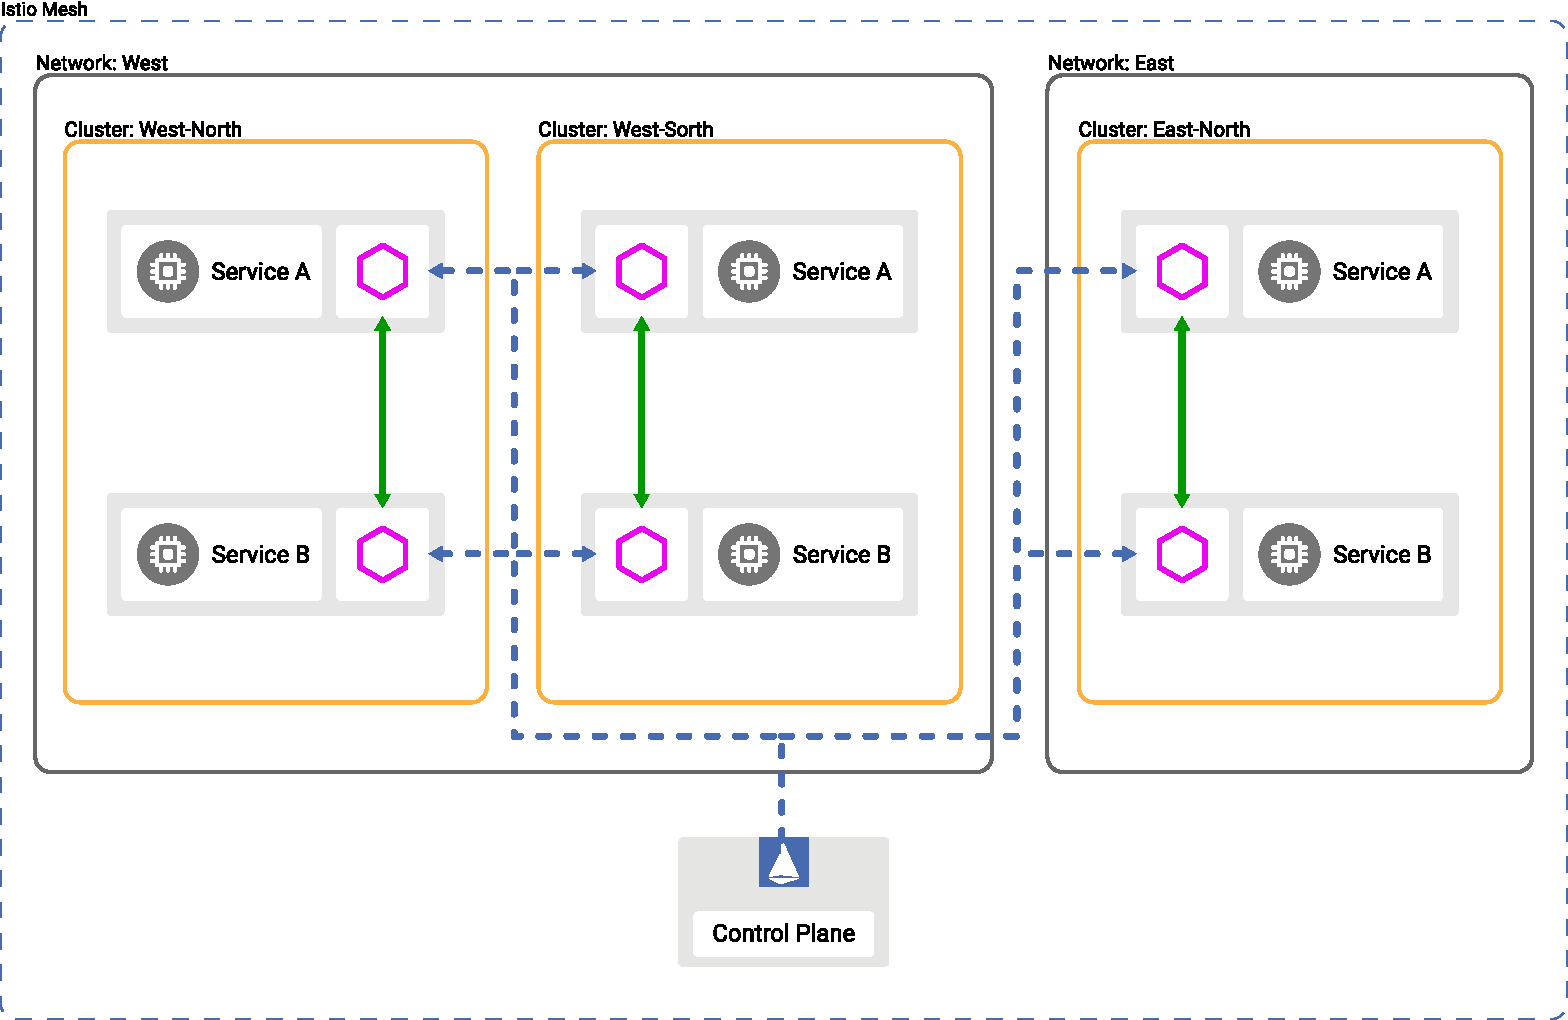
\includegraphics[width=0.75\linewidth]{figs/pdf/istio-multi-cluster}
  \caption{Multiple clusters on Istio}
  \label{fig:istio}
\end{figure}


\subsubsection*{Comparison}

It is mostly generic to applications that can be used in
Kubernetes\footnote{\url{https://istio.io/latest/docs/ops/deployment/requirements/}
  - Accessed: 2022-09-20}.
%
Since it extends Kubernetes, there is no changing the code for many
applications, however, some might require some changes, depending if
the application requirements are met or not yet.
%
This requirements \emph{for some applications} have given Istio a
three/two clouds for non-intrusion, for fairness.
%

Since multi-cluster is only supported with a central control plane, we
do not consider that it can survive a network partition.
%
Of course, though, if one site is cut off from the rest, users can
still use another site.
%
In mesh
federation\footnote{\url{https://istio.io/latest/docs/ops/deployment/deployment-models/\#multiple-meshes}
  - Accessed: 2022-09-20}, it might be possible, but even with the
Google
demo\footnote{\url{https://github.com/GoogleCloudPlatform/istio-samples/tree/master/multicluster-gke/dual-control-plane}
  - Accessed: 2022-09-20}, the information given on the functionality
is not sufficient to determine this (especially because it seems to
mostly allow service spreading across potentially different sites, but
at minimum different meshes).

The configuration of the deployment is prepared statically, and can be
updated depending on the users needs.

The location of execution of requests is determined through Envoy
load-balancing, so it is automatically chosen.

Since Istio has been designed for the Cloud, its control plane is
centralized, and thus, most of the functionalities are executed there.
%
Finally, there is no real point in talking about Istio \acrshort{P2P}
capabilities, except for this
example\footnote{\url{https://banzaicloud.com/blog/istio-multi-mesh/}
  - Accessed: 2022-09-20}, where they achieved a multi-mesh,
multi-cluster which can be considered as a \acrshort{P2P} version of Istio, so it
is technically possible, though not designed for this.
%

\subsubsection*{Conclusion}

Istio is a service-mesh using Envoy as a sidecar proxy for every
services.
%
Some efforts have already been made to allow multi-cluster in Istio,
though it is still not designed to be entirely autonomous and
decentralized as the control plane is centralized (at best one per
region).
%
Thus, it is going in a really good direction for us, with some
possibilities to make a P2P version, it is still lacking user chosen
locations for executing requests, as it is done automatically.



\subsection{Linkerd~\cite{linkerd}}
\label{sec:soa-linkerd}

Linkerd is another service mesh, which was the first called like that.
%

Linkerd, like Istio, allows to filter and route \acrshort{TCP},
\acrshort{TLS}, HTTP(/2) and \acrshort{gRPC} requests, with much more
functionality on the last two.


Linkerd2 uses
Linkerd2-Proxy\footnote{\url{https://github.com/linkerd/linkerd2-proxy}
  - Accessed: 2022-09-20}, an ``ultralight micro-proxy'' tailored for
their needs to make Linkerd smaller and simpler.
%
Linkerd developers decided that Envoy had too much
functionalities which made it inappropriate for a sidecar use.
%
Whether it is for the complexity, the resource consumption, or the
danger of having such a complex proxy introducing security issues in
its code, they preferred a lightweight approach that work perfectly
for their use case.
%
The downside is that it is not recommended to use Envoy as a proxy and
Linkerd2-proxy would not be usable by another service
mesh\footnote{\url{https://linkerd.io/2020/12/03/why-linkerd-doesnt-use-envoy/}
  - Accessed: 2022-09-21}.

\autoref{fig:linkerd} shows an overview on how Linkerd deal with the
Multiple Cluster functionality.
%
Clusters (here, west and east) communicates with each other through a
Multi-Cluster gateway.
%
This gateway is then responsible to route a request from a Service
from the other cluster to the involved Service in its own cluster.
% https://github.com/linkerd/website/blob/main/linkerd.io/static/images/multicluster/feature-overview.svg
% https://linkerd.io/2.12/features/multicluster/
\begin{figure}[htbp]
  \centering  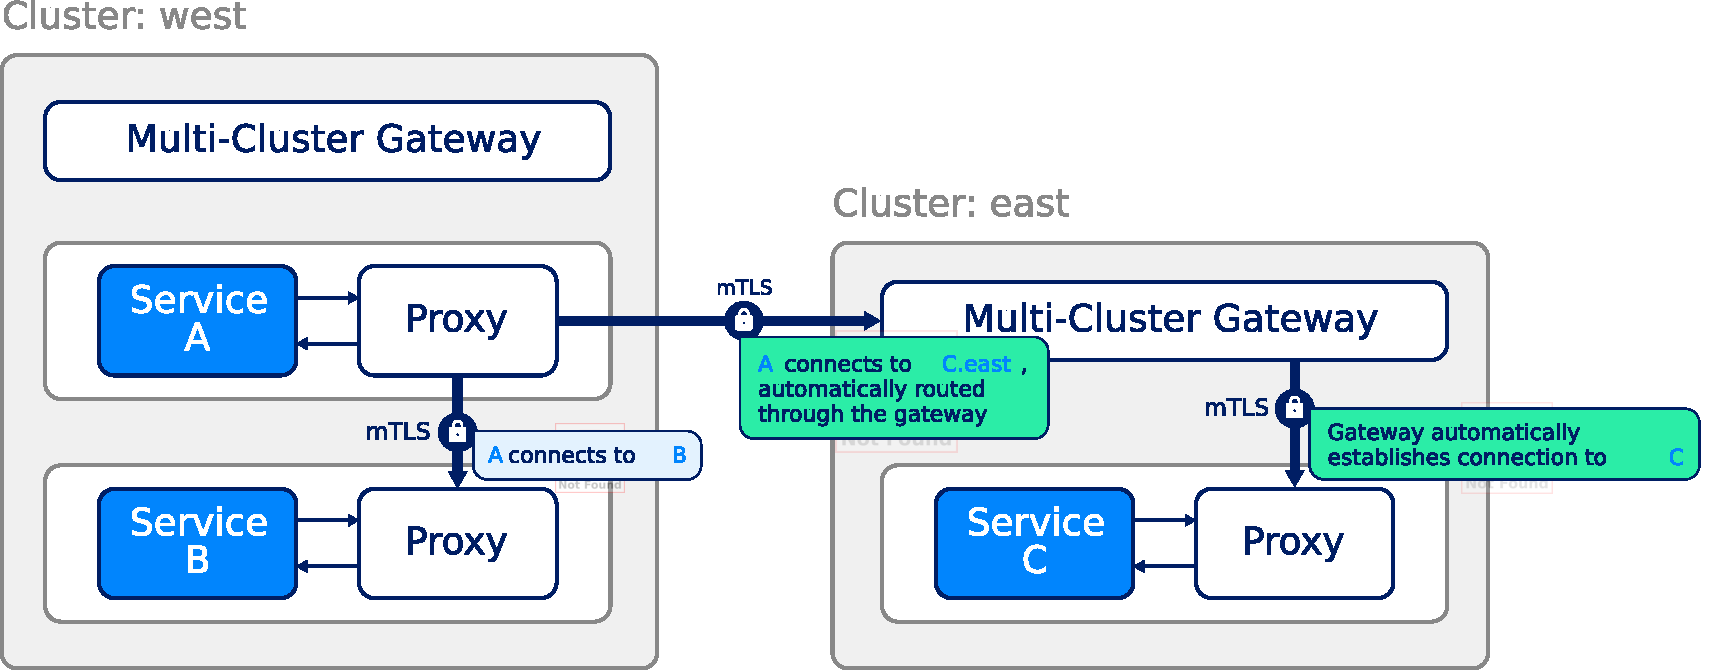
\includegraphics[width=0.75\linewidth]{figs/pdf/linkerd-multi-cluster}
  \caption{Multiple clusters on Linkerd}
  \label{fig:linkerd}
\end{figure}

\subsubsection*{Comparison}

Linkerd, as for most service meshes, does not require any change in
the business code of the underlying applications, though it is also
specific to Kubernetes, because it only consider resources managed by
Kubernetes (with mesh expansion on the
roadmap\footnote{\url{https://github.com/linkerd/linkerd2/blob/main/ROADMAP.md}
  - Accessed: 2022-09-21}).

It is design to work locally first since it is supposed to be running
in the Cloud, but in multi-cluster, it is possible to get resources
from other services.


The recommendations on how to make an architecture for multi-cluster
Kubernetes give these architectures with Linkerd a solid chance of
surviving network
partitions\footnote{\url{https://linkerd.io/2020/02/17/architecting-for-multicluster-kubernetes/}
  - Accessed: 2022-09-21}.
%
They recommend to maintain independent states between clusters and
manage updates via replications so updates are only where required.
%
They also advise to keep the control planes independent separate,
which further makes the system more tolerant to network partitions.
%
When the control plane is down, though, the proxies will use the
information they already have and fall back to \gls{Domainns} (\acrshort{DNS}) if a
request is supposed to be routed to a service they do not know.
%
But this implies that any proxy deployed when the control plane is
down will need to timeout all new requests until the control plane is
up
again\footnote{\url{https://linkerd.io/faq/\#what-happens-to-linkerd-s-proxies-if-the-control-plane-is-down}
  - Accessed: 2022-09-21}.
%
In conclusion, Linkerd in multi-cluster mode is tolerant to network
partitions, but not entirely.

Regarding dynamicity, Linkerd uses an algorithm called Exponentially
Weighted Moving Average (EWMA) to automatically route requests to the
fastest
endpoints\footnote{\url{https://linkerd.io/2.12/features/load-balancing/}
  - Accessed: 2022-09-21}.
%
The execution location of a request is chosen for the user, in part
through traffic split.

As for Istio, we cannot consider this application of the \acrshort{P2P} point,
since it has not really been designed to work with several instances
of the application.

\subsubsection*{Conclusion}

Linkerd is a service mesh that relies on a homemade, lightweight and
less generic proxy than Envoy, called Linkerd2-Proxy.
%
It also supports a multi-cluster architecture if need be, through
gateways on each cluster that redirects the request they receive
locally to the required service.


\subsection{Conclusion on service meshes}
\label{sec:soa-sm-conclusion}

We studied two different service meshes which mostly have the same
functionalities and goals, except that Linkerd seems to be more
focused on being lightweight.
%
In the appendix (\autoref{chap:first-approach}), we
will also talk a bit about Consul, which has been considered as a
solution for us for a time.

\begin{table}[htbp]
  \centering
  \footnotesize\setlength{\tabcolsep}{4pt}
\begin{tabular}{|c|c|c|c|c|c|c|c|c|c|}
\hline
 & NI & generic & LF & CT & NP & dynamic & on-demand & decentralized & P2P\\
\hline
Istio & \cloud \cloud \cloud /\cloud \cloud  & \cloud \cloud  & \cloud \cloud \cloud  & \cloud \cloud  & \cloud  & \cloud \cloud  & \cloud  & \cloud  & -\\
Linkerd & \cloud \cloud \cloud  & \cloud \cloud  & \cloud \cloud \cloud  & \cloud \cloud  & \cloud \cloud  & \cloud \cloud  & \cloud  & \cloud \cloud  & -\\
  \hline
  \end{tabular}
  \caption{Comparison points on service meshes.}
  \label{tab:soa-sm}
\end{table}

Overall, service meshes could be a good solution to our main research
question of putting Cloud applications to the Edge if they were
designed for the Edge, to be more collaborative, more decentralized,
and more generic.
%
It is especially true since they are doing more and more efforts to
support multi-clustering (both propose versions of this functionality,
with different levels of support) and more application managers.

It is also noteworthy that despite some efforts, service meshes are
pretty demanding and impact the performance of small devices, so there
is a lack in service meshes that would be able to be used at the
Edge~\cite{GRRL+21}.
%
A lightweight version that checks our requirements might be the
solution to our research questions, and especially this one: ``since
service meshes are designed to manage the communications between
services of an application outside of its business code, can it be a
solution to using Cloud applications on Edge infrastructures without
changing their code?''.


As we did not find an approach that fits entirely the requirements, we
will now consider techniques to make applications at the Edge in order
to learn if some ideas could help us in building a generic solution on
the main question raised in this manuscript.



\chapter{How to make Edge applications natively}
\label{chap:soa-dev-edge-app}

Though we think it is better to not reinvent the wheel, and so use as
much as possible Cloud applications directly on the Edge, it is still
possible to develop an Edge application from scratch.
%
First, it makes sense of course simply for new applications that will
be developed with the Edge in mind.
%
Second, some frameworks might have been developed to do so, in case
some of them might automatize the process of pushing an application to
the Edge, which could work on an existing Cloud application.
%
Third, some approaches might give guidelines on how to properly
develop an application for the Edge~\cite{RYHL19}, which is of interest even to know
how to push an existing Cloud application to the Edge.

\section{Towards Scalable Edge-Native Applications~\cite{WFGI+19}}
\label{sec:WFGI+19}

\cite{WFGI+19} from Wang et al. presents an approach to ``edgify'' an
application, \ie the Gabriel platform~\cite{HCHR+14}, that was
designed for a single user.
%
Though this approach is mainly about multi-tenancy, because Gabriel
was already an application to offload the functionalities of IoT to
Fog/Edge, it gives requirements for the Edge.
%

Since the authors are changing Gabriel to be more scalable, they talk
about the enhance version as "Scalable Gabriel", while the other is
"Original Gabriel".
%
In this paper, they refer to a three tier architecture of the Cloud
computing.
%
The Tier-3 would be the Edge, composed of IoT and mobile devices, and
where data are pre-processed in the Gabriel front-end (\eg compression
and encoding).
%
The Tier-2 would correspond to the Fog (what we refer to as the Edge),
composed of cloudlets, small \acrshort{DC}s, etc., and where the
Gabriel back-end and its different modules treat the data from the
Tier-3.
%
The Tier-1 would be the Cloud itself, with further and bigger
\acrshort{DC}s, with more compute power, energy usage and elasticity.

The original Gabriel was built for a single user, \ie only one sensor
interacting with one cloudlet (1:1), and they want to allow several
devices to interact with the same cloudlet (n:1).

Several applications run on the original Gabriel Platform, but the
authors focus on Wearable Cognitive Assistance (WCA, running typically
on glasses for Augmented Reality in their cases) applications because
they deem that these applications present three crucial
characteristics for Edge computing:
\begin{itemize}
\item they transmit large volumes of (video) data from the device to
  the cloudlet (Tier-3 to Tier-2, or in our case, we would say from
  the devices to the Edge).
\item they have strict latency requirements
\item they impose high computing demands on the cloudlet, especially
  in the GPUs.
\end{itemize}
Regarding the last characteristic, the workflow of these applications
in the cloudlet is composed of two phases.
%
The first phase treat the images to extract an abstract, symbolic
representation of the state of the task, while the second phase, far
less compute intensive, operates on this symbolic representation,
implementing the logic of the task.

To tackle the scalability problems, they first reduce the load going
through the wireless network and to the cloudlet through adaptation
(\emph{Workload reduction}); the second is about a better scheduling
of cloudlet resources to minimize queuing and impacts of potential
overloads (\emph{cloudlet resource allocation}).
%
Both those approaches are tested afterwards.

To adapt the original Gabriel to these points, they leverage the WCA
applications characteristics.
%
The first is the \emph{human-centric timing}, which corresponds to the
fact that the applications have active phases, where they need to
sample and process video frames to give instructions to the users,
which will perform these instructions in the passive phase of the
applications.
%
In this passive phase, the sampling and processing of video frames to
determine if the user has soon finished the instructions, which would
considerably reduce the load.

The second is \emph{event-centric redundancy}, where they detect
redundant frames that do not provide new information to reduce the use
of the wireless bandwidth and the cloudlet cycles on frames.

The third is \emph{inherent multi-fidelity}, in which they leverage
the fact that some of the processing algorithms can trade-off fidelity
and computation.
%
When a cloudlet becomes overloaded by multiple
applications, it is possible to act on this trade-off to ensure the
applications functionalities.

Finally, they give a taxonomy of relevant adaptations depending on the
characteristics of the applications. These adaptation techniques are
presented in ~\autoref{table:WFGI+19}.

\begin{table}[h!]
  \begin{center}
    \begin{scriptsize}
      \begin{tabular}{|c|p{4.5cm}|p{5.5cm}|p{4cm}|}
        \hline
        & & & \\
        & \textbf{Question}      & \textbf{Example}   & \textbf{Load-reduction Technique}    \\
        & & & \\
        \hline
        1         & How often are instructions given, compared to task duration?    & Instructions for each step in IKEA lamp assembly are rare compared to the total task time, e.g., 6 instructions over a 10 minute task.    & Enable adaptive sampling based on active and passive phases.    \\
        \hline
        2 & Is intermittent processing of input frames sufficient for giving instructions? & Recognizing a face in any one frame is sufficient for whispering the person’s name. & Select and process key frames.   \\
        \hline
        3 & Will a user wait for system responses before proceeding? & A first-time user of a medical device will pause until an instruction is received. & Select and process key frames. \\
        \hline
        4 & Does the user have a pre-defined workspace in the scene? & Lego pieces are assembled on the Lego board. Information outside the board can be safely ignored. & Focus processing attention on the region of interest.\\
        \hline
        5 & Does the vision processing involve identifying and locating objects? & Identifying a toy lettuce for a toy sandwich. & Use tracking as cheap approximation for detection.\\
        \hline
        6 & Are the vision processing algorithms insensitive to image resolution? & Many image  classification DNNs limit  resolutions to the size of their input layers. & Downscale sampled frames  on  device before transmission.\\
        \hline
        7 & Can the vision processing algorithm trade off accuracy and computation? & In image classification, MobileNet is computationally cheaper than ResNet, but less accurate. & Change computation fidelity based on resource utilization.\\
        \hline
        8 & Can IMUs be used to identify the start and end of user activities? & User’s head movements are of significantly higher magnitude when searching for a Lego block. & Enable  IMU-based  frame suppression.\\
        \hline
        9 & Is the Tier-3 device powerful enough to run parts of the processing pipeline? & A Jetson TX2 can run MobileNet-based image recognition in real-time. & Partition the vision pipeline between Tier-3 and Tier-2.\\

        \hline
      \end{tabular}

      \centering
      \caption{Application characteristics and corresponding
        applicable techniques to reduce load (Source: Wang et
        al.~\cite{WFGI+19}).}
    \label{table:WFGI+19}
  \end{scriptsize}
  \end{center}
\end{table}

Then, they proceed in testing these techniques for workload reduction,
as mentioned above.
%
From these evaluations, the authors are able to conclude that
Edge-native applications should be written in very different way from
Cloud-native applications to be scalable.


\subsubsection*{Comparison}

Since this paper is about specific use-cases (WCA applications) that
requires some computing locally and most of it in what we call Edge
computing, the question of collaboration is difficult, since
collaborations is only vertical (from one Tier to another) and not
horizontal (between multiple sites of the same Tier).
%

The approach is about modifying an existing application (original
Gabriel), but the overall logic did not change.
%
It is generic for any (WCA) application that can run on the Gabriel
platform only, but the adaptations are much wider and could be used
both to adapt a Cloud application or to build and Edge application.

%
Monitoring of the resources is done on both tiers of the involved
architecture (Tier-3 and Tier-2), but some are monitored at Tier-3,
others at Tier-2.
%
As said before, the collaboration is only vertical and most resources
are not managed locally, so it is only some part of the computation
that is available locally \textbf{and} it only a subset of resources
is used in collaboration.

%
Once again, because of the verticality, network partition is tricky.
%
If we consider network partition in the same tier, it will not be a
problem, since there is no collaboration inside.
%
But, in the context of WCA applications, on a wireless network, there
is a even larger chance of a partition between any of the devices and
the cloudlet, and thus, any offload computation could not be
done. Thus, only one cloud is awarded, for the case of partition in
the same tier.

The authors do not debate the n:n relationship between devices and
cloudlets, so there is no real dynamic choice of the location of
execution of requests, and the same can be said for the user ability
of choosing the location.

% Since WCA applications are designed to make computation further away
% from the devices, it is difficult to call them ``Cloud
% applications''. And if we consider using the Gabriel platform, it is
% the same problem; as well as the fact that they changed it.

The cloudlet is the actual only place of execution of the tasks, no
mention of a re-balancing to other cloudlets, so the approach is
hierarchical and centralized.

Because the Tier-3 Gabriel front-end is not the same as its back-end
Tier-2 counterpart, and most of the workload is done in the cloudlet,
we cannot say this approach is a \acrshort{P2P} system.

\subsubsection*{Conclusion}

In conclusion, this approach is a redesigned version of Gabriel, a
platform to allow a single wearable device process data in a cloudlet,
to allow the cloudlet to manage several devices.
%
By degrading the quality of service when it is possible and not
required, the cloudlet is able to withstand a much higher load and
number of connected devices than previously, as well as the wireless
network load is decreased.
%
They defined a taxonomy of applications and a set of rules to apply to
allow a smarter processing of the data recorded by edge devices, which
could be reusable to adapt a Cloud application for the Edge as well as
to develop a new Edge-native application from scratch.
%
This approach, by only considering only vertical relations
(edge-devices to cloudlet), is not using the entire capabilities of
the Edge and is designed specifically for small edge devices that need
to offload almost all their workloads to the Edge servers/Fog.

This solution is pretty interesting for the ideas on how to adapt an
application for the Edge, even though it is mainly aimed at WCA
applications because they leverage some of their unique
characteristics.
%
One conclusion in this paper I found really interesting is they
consider that Edge-native applications should be written very
differently from Cloud-native ones to be scalable.
%
It is probably true for applications running on the Edge devices, but
it would be interesting to test on Edge servers, since it would be
that we cannot have a non-intrusive approach.


\section{Highly-Available and Consistent Group Collaboration at the
  Edge with Colony~\cite{TSS21}}
\label{sec:TSS21}

Colony~\cite{TSS21, Toumlilt21} by Toumlilt et al. is composed of a
middleware and a database to address the lack of approaches for
collaborative applications at the Edge.
%


\begin{figure}[htbp]
  \centering  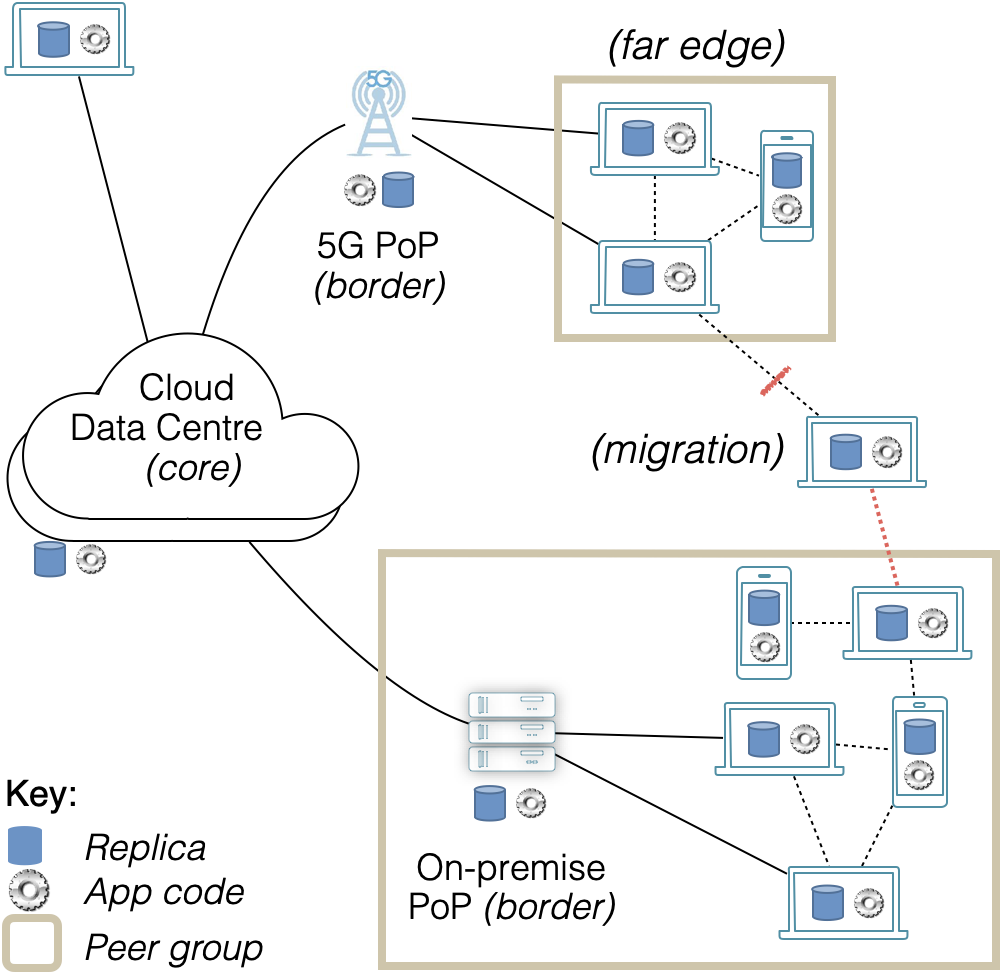
\includegraphics[width=.6\linewidth]{figs/png/colony-topology}
  \caption{An example of a Colony topology (Source:~\cite{Toumlilt21}).}
  \label{fig:colony}
\end{figure}

The database responds to the need of Edge-to-Cloud continuum and is
designed for collaborative applications.
%
In a typical usage, presented in~\autoref{fig:colony}, the Cloud core
is composed of a small number of \acrshort{DC}s, and the Edge nodes
are grouped by proximity, connecting either to the core \acrshort{DC}s
or to a PoP server at the border of the group.
%
Due to mobility, a node can migrate from one group to another.


The focus of this work is consistency in the Edge with a local-first
approach.
%
As such, they enforce a hybrid approach for consistency: globally, the
model follows a Transactional Causal Plus Consistency (TCC+)
introduced in the paper; in the data centers, the consistency provided
is Snapshot Isolation (SI), as the servers are connected through
high-quality networks; finally, in the local groups, they also enforce
SI, but the system needs to be able to work disconnected to keep them
available and without losing the overall TCC+ guarantees, using
EPaxos.

The TCC+ model guarantees causal consistency~\cite{ANBKH95},
rollback-freedom (no rollbacks after a value has been read), strong
convergence (any two nodes observing the same set of updates read the
same value), atomicity, snapshot.
%
It extends the TCC model~\cite{ZPDBVS15} with the strong convergence
and rollback-freedom


\subsubsection*{Comparison}

The Colony middleware is designed to provide a simple \acrshort{API}
to develop and deploy collaborative applications at the Edge.
%
This means that some effort is made to help developers to make their
applications collaborative at the Edge, but it is thus a very
intrusive method to follow the necessary data types and \acrshort{API}.
%
%It also means that it is not made to use existing Cloud applications.
%
This approach is generic to any type of collaborative applications for
the Edge.

The local-first principle is one of the focus of the approach, and it
is enforced by replications and caches.
%
There are collaborations (in our sense) between the nodes in the same
group especially when needed, on any types of resources.

The application is supposed to be able to work offline with the entire
system and design, so in effect, it supports network partitions: ``the
application can read and write data, even when disconnected from any
remote server''.

The required information are transmitted to required nodes
dynamically, even in case of mobility.
%
The location of execution of requests is mainly local, and on the
peers of the collaborative applications.
%
Data is replicated and cached depending on the edge client
\emph{interest}.

The approach is hierarchical, as some transactions are run only in
the core Cloud, such as analytics or large queries.
%
The core also manages the authentication of nodes via the session
manager, but it is only for the current implementation.


\subsubsection*{Conclusion}

In conclusion, Colony is an approach to design collaborative
applications for the Edge, guaranteeing the highest consistencies
possible for the availability of the resources in the context of the
Edge.
%
To do so, it follows a hybrid approach in consistency, using TCC+ in
the global cases ans Snapshot Isolation in the peer, Edge groups.
%
It allows migration of nodes between groups for mobility and ensures
fault-tolerance and scalability by having the groups replicated
roots in the Cloud.
%

Overall, it is a really interesting approach to design collaborative
applications for the Edge, which is robust, mostly decentralized,
generic and follows the base principles of local-first and
collaborative-then.

As a final note, this approach uses a shared database approach, which
we did not want to use for reasons presented
in~\autoref{ssec:issue-db}, but makes sense if properly used for a
new application, developed from scratch.

% The trade-off is that, during some failures, liveness cannot be
% ensured. A client cannot make progress in two cases: if it requires
% data that cannot be retrieved; or if it runs out of storage. Further-
% more, there are corner cases (described later) where a client commits
% updates, but they cannot become visible. The above situations are
% temporary, and last only until the problem is repaired.





\section{Conclusion on ways to make an application at the Edge}
\label{sec:soa-edge-conclusion}


To ease the reading of the table, we add the following reminder:
\begin{description}
\item [\cite{WFGI+19}] Towards Scalable Edge-Native Applications (\autoref{sec:WFGI+19})
\item [\cite{TSS21}] Highly-Available and Consistent Group Collaboration at the Edge with Colony (\autoref{sec:TSS21})
\end{description}


\begin{table}[htbp]
  \centering
  \footnotesize\setlength{\tabcolsep}{4pt}
    \begin{tabular}{|c|c|c|c|c|c|c|c|c|c|}
      \hline
       & NI & generic & LF & CT & NP & dynamic & on-demand &  decentralized & P2P\\
      \hline
      \cite{WFGI+19} & \cloud & \cloud \cloud  & \cloud  & \cloud \cloud  & \cloud  & - & - & \cloud  & \cloud \\
      \cite{TSS21} & \cloud & \cloud \cloud \cloud  & \cloud \cloud \cloud  & \cloud \cloud \cloud  & \cloud \cloud \cloud  & \cloud \cloud \cloud  & \cloud \cloud  & \cloud \cloud  & \cloud \cloud \\
      \hline
  \end{tabular}
  \caption{Comparison points on making applications at the Edge.}
  \label{tab:soa-edge}
\end{table}

\autoref{tab:soa-edge} sums up the comparison on the approaches to
make applications at the Edge.

Both approaches are pretty different and do not focus on the same
requirements.

%
In~\cite{WFGI+19}, the focus is about making intelligent choices (both
in design and by the use of adaptive algorithms) to lower the load
when possible and allow several applications to run on the same node.
%
Thus, it also gives clues on how to adapt an existing Cloud
application for the Edge, but keeping only its functionality logic and
changing entirely the way it is used.

%
In~\cite{TSS21}, the authors focus on bringing consistency,
scalability and offline mode to collaborative applications at the
Edge.
%
Moreover, the approach follows the local-first principle, same as us,
which makes it a particularly strong candidate to answer our
requirements, but it lacks the decentralized, \acrshort{P2P} system
that leaves the users the ability to choose the execution location of
their requests.


Both answer parts of the puzzle of building an Edge-native
applications.




\chapter{Comparison and conclusion on the State of the Art}
\label{chap:soa-conclusion}

\section{Comparison }
\label{sec:soa-comparison}


To ease the reading of the table, we add the following reminder, for
approaches that can't be in a single word:
\begin{description}
\item [\cite{Spataru20}] Decentralized and Fault Tolerant Cloud
  Service Orchestration (\autoref{subsec:spataru20} - Decentralized
  CloudLightning)
\item [\cite{SYHJ17}] Re-designing Cloud Platforms for Massive Scale
  Using a P2P Architecture (\autoref{subsec:SYHJ17} - P2P OpenStack)
\item [\cite{WFGI+19}] Towards Scalable Edge-Native Applications
  (\autoref{sec:WFGI+19} - Scalable Gabriel)
\end{description}

\begin{table}[htbp]
  \centering
  \footnotesize\setlength{\tabcolsep}{2pt}
\begin{tabular}{|c|c|c|c|c|c|c|c|c|c|}
\hline
Approach & NI & generic & LF & CT & NP & dynamic & on-demand & decentralized & P2P\\
\hline
  \cite{Spataru20} & \cloud \cloud \cloud  & \cloud \cloud \cloud  & - & \cloud \cloud \cloud  & \cloud  & \cloud \cloud \cloud  & \cloud  & \cloud \cloud \cloud  & \cloud \cloud \cloud \\
  Liqo~\cite{IRPCM22} & \cloud \cloud \cloud  & \cloud \cloud  & \cloud \cloud \cloud  & \cloud \cloud \cloud  & \cloud \cloud \cloud  & \cloud \cloud  & \cloud \cloud  & \cloud \cloud \cloud  & \cloud \cloud \\
  HYDRA~\cite{JS20} & \cloud \cloud \cloud  & \cloud \cloud  & \cloud  & \cloud \cloud \cloud  & \cloud \cloud \cloud  & \cloud \cloud  & \cloud  & \cloud \cloud \cloud  & \cloud \cloud \cloud \\
  OneEdge~\cite{SGDR21} & \cloud \cloud \cloud  & \cloud \cloud \cloud  & \cloud \cloud  & \cloud \cloud \cloud  & \cloud  & \cloud \cloud \cloud  & \cloud  & \cloud \cloud  & \cloud \cloud \\
  OpenYurt\cite{openyurt} & \cloud \cloud \cloud  & \cloud \cloud  & \cloud \cloud & \cloud \cloud \cloud  & \cloud & \cloud \cloud  & \cloud  & \cloud  & \cloud \\
  \cite{SYHJ17} & \cloud \cloud \cloud  & \cloud \cloud  & \cloud \cloud \cloud  & \cloud \cloud  & \cloud \cloud \cloud  & \cloud \cloud  & \cloud \cloud  & \cloud \cloud \cloud  & \cloud \cloud \cloud \\
  \hline
  Istio~\cite{SS20} & \cloud \cloud \cloud  & \cloud \cloud  & \cloud \cloud \cloud  & \cloud \cloud  & \cloud  & \cloud \cloud  & \cloud  & \cloud  & -\\
  Linkerd\cite{linkerd} & \cloud \cloud \cloud  & \cloud \cloud  & \cloud \cloud \cloud  & \cloud \cloud  & \cloud \cloud  & \cloud \cloud  & \cloud  & \cloud \cloud  & -\\
  \hline
  \cite{WFGI+19} & \cloud  & \cloud \cloud  & \cloud  & \cloud \cloud  & \cloud  & - & - & \cloud  & \cloud \\
  Colony~\cite{TSS21} & \cloud  & \cloud \cloud \cloud  & \cloud \cloud \cloud  & \cloud \cloud \cloud  & \cloud \cloud \cloud  & \cloud \cloud \cloud  & \cloud \cloud  & \cloud \cloud  & \cloud \cloud \\
  \hline
  \end{tabular}
  \caption{Comparison points on the overall state of the art.}
  \label{tab:soa-comp}
\end{table}

\autoref{tab:soa-comp} represents the overall comparison according to
the different categories.

There is no solution that fits entirely the requirements,
but there are some that fit perfectly or almost our principles of
local-first and
collaborative-then~\cite{TSS21,IRPCM22,SGDR21,openyurt,SYHJ17}.

A lot of the different solutions considered overall had a
non-generic approach, except for how to build a Edge-native
application, of course.
% all of the solutions are non-intrusive because
% it was crucial for us.


A requirement that is also mostly overlooked is the resilience to
network partitions, with four approaches that do not have a way to
cope with it, even when we do not count service meshes that were
designed for the Cloud (and thus need it less).
%
In the context of the Edge, it is unreasonable to neglect site
autonomy when disconnections are the norm rather than the exception.


In terms of putting Cloud applications to the Edge, the solutions
studied leverage a distributed database in two
cases~\cite{Spataru20,TSS21}, while others use some sort of brokering
or service-to-service~\cite{SYHJ17, WFGI+19} without the
location-aware aspects to make it less intrusive.
%
And interestingly, the non-intrusive requirement is the one that is
mostly observed, except for solutions to build applications for the
Edge, which makes sense for Edge-native applications.

As for the genericity, it is mainly provided by allowing to deploy
containerized applications~\cite{IRPCM22, JS20, openyurt, linkerd,
  SS20} or applications in containers, VMs, and sometimes more (like
bare metal)~\cite{Spataru20, SGDR21}.

As mentioned in the more specific comparisons, the user-centric to
have on-demand, dynamically managed requests is what is mostly lacking
from the approaches, though dynamicity is considered
at request level in three solutions.
%
This is the point that definitely needs to be taken into account for
our solution, if we want to allow users to define where they want
their requests to be executed.


% If we exclude the service meshes that were not designed specifically
% for the Edge, the consideration of the network partition is stunningly
% not enough considered, since disconnections at the Edge must be
% considered the norm rather than the exception.


\section{Conclusion }
\label{sec:soa-conclusion}

In this part, we have seen different solutions to allow applications
running at the Edge.

%
One of the goals was to find original (and different from one another,
except for the service meshes), generic and/or usable approaches that
have not been studied already by members of our project, such as in
Manaouil et al.\cite{ML20}.


%
This State of the Art does not cover specific subjects in the
deployment and life cycle of applications services, such as algorithms
in charge of discovery, monitoring, load-balancing or placement, but
rather tried to focus on solutions that fit at least some of them, to
have ideas on how it is dealt with.
%
Of course, still in the context of having applications at the
Edge.
%
It is also sidelining approaches to manage the physical, hardware Edge
infrastructure that study how to put computing devices in the
infrastructure because it was out of scope, and we considered that
we had the infrastructure ready to use.
%

%
Some of the solutions presented here are really good answers to the
Edge challenges in their own way, and only fail our own requirements.

%
The hierarchical approaches, for example, create Single Point of
Failure (\acrshort{spof}) and bottlenecks, and thus cannot be
envisioned as solutions unless they have mechanisms to avoid those
problems (replication~\cite{TSS21}, temporary autonomy~\cite{SS20},
etc.).
%
The lack of tolerance to network partitions/disconnections is also a
problem in the context of the Edge, as mentioned before.
%
Finally, the lack of dynamic and on-demand, only when required
collaborations, with most of the workload executed as locally as
possible, is what drove the approach we built and will now detail.

What can be taken away from this State of the Art, regarding the
requirements:
\textbf{
\begin{itemize}
\item While a lot of approaches are collaborative, not enough respect
  the local-first principle or the tolerance to network partitions,
  which is a problem in the context of the Edge.
\item Approaches that are generic concentrates mostly on deploying
  containerized applications, especially with Kubernetes, without
  considering the collaborations that could be done between the
  deployed application.
\item Solutions often consider dynamicity of the requests, which is a
  good thing in a highly dynamic context, but they do not consider
  enough the will of the users by allowing the execution location to
  be chosen on-demand by the users.
\end{itemize}
}
None of the solutions answered to all the requirements, but the
service mesh approaches could be leveraged to make a service dedicated
to managing the geo-distribution in a decentralized and P2P manner,
outside of the business code, similar to the multi-cluster approach of
Linkerd.
%
This point of view will be more detailed and explained in the next
part, with our own solution.

% The requirements on dynamicity and per-demand user requests are
% important to us, but the user-centric requirement is definitely not
% the priority in the solutions studied.
%






% \chapter{Using Cloud Applications at the Edge}
% \label{chap:soa-c-to-e}

% \todoref{cf sources in comments}
% % https://itnext.io/superedge-openyurt-extending-native-kubernetes-to-edge-cc59094f92c
% % https://medium.com/volterra-io/control-plane-for-distributed-kubernetes-paas-e20a82acd6d3
% % https://landscape.cncf.io/?license=open-source&grouping=no
% % https://liqo.io/
% % https://krossboard.app/docs/01_overview-concepts-features/

% \todono{titles}
% \section{Using databases}
% \label{sec:soa-dbs}

% \section{Using broker}
% \label{sec:soa-broker}

% \section{Using service-to-service}
% \label{sec:soa-s-to-s}

% %\section{Using containers}

% \chapter{Using service meshes at the Edge}
% \label{chap:soa-SM}


% \subsection{Istio}


\clearemptydoublepage
\part{Developing a solution to use native Cloud Applications at the Edge}
\label{part:cheops}

\epigraph{For within each seed, there is a promise of a flower.}{\emph{Dillon, Alien$^3$}}



In this part, we are going to see how we designed a solution that
fulfill the requirements defined in~\autoref{sec:principles}.

%
In~\autoref{chap:overview}, I present the overview of the approach,
and the concepts to give some insights on to reproduce an
implementation.
%
This includes the basics on how the approach function, on what it
relies from Cloud applications and what is required achieve the
requirements we explained earlier.
%
Specifically, I will detail the Domain Specific Language
(\acrshort{DSL}) made to allow for outside management of
geo-distribution concerns, and an overview of some collaborations it
offers and an insight in other possible useful collaborations is also
presented.
%
Furthermore, a glimpse into the classification of resources
dependencies is given to understand how we can help users with the
manipulation of resources.

Then, in~\autoref{chap:cheops}, I will expose the vision and current
implementation, called Cheops, a service mesh to geo-distribute Cloud
applications at the Edge.
%
% In the process, I will also give information on how this prototype
% came to be, including a first version which used an existing service
% mesh.
%
Finally, I will examine the validation we made on our implementation,
that is a common work between Geo Johns Antony, a PhD student
colleague, and me.

This part includes work from different communications made in the
scientific community~\cite{CLRB19, CDLR+20, CDL21, DCL21,
  compas-poster, DAL22} and the OpenInfra Summit
2022~\cite{OIS-Berlin22}, along with different people in the team,
namely Geo Johns Antony, Ronan-Alexandre Cherrueau, Adrien Lebre, and
Javier Rojas Balderrama, without forgetting the implication of
Matthieu Simonin.


\chapter{An approach dedicated to geo-distribution}
\label{chap:overview}


This chapter exposes the logic of the approach, how it works, what is
needed to achieve it.
%
First, I will explain how the modularity of applications is one of the
main characteristics of this approach by allowing the externalization
needed.
%
Then, I will present \scl, the Domain Specific Language made to extend
requests with the geo-distribution information.
%
Finally, I will explicit what types of collaboration we have
envisioned for the solution.

It is worth mentioning that most of this chapter comes from our
Euro-Par article~\cite{CDL21}.
% , written with Ronan-Alexandre Cherrueau
% and Adrien Lebre.

% definition
% services based
% REST API

\section{A service-mesh approach}
\label{sec:service-mesh}

% One of the available solution to deal with service composition
% dynamically is to use a reverse proxy.
% %
% A reverse proxy is a broker between clients and services of the
% application that changes the service composition on the fly.
% %
% It is implemented usually for reliability and performance, by, for
% example, balancing incoming requests to multiple instances of the same
% service within one application instance.
% %

As we discussed in~\autoref{sec:cloud-app}
and~\autoref{chap:cloud-app-to-edge}, service-based applications, like
a lot of Cloud applications, are composed of different services.
%
These services aim to provide modularity to the applications, and the
decoupling of functionalities.
%
This modularity principle comes from software engineering, allowing
separation of concerns (for example to have different teams working on
separate aspects in the business code), reusing of existing modules,
and overall better development manageability.
%


The services communicate between each other through the \acrshort{API}
they expose that allows access specific function to manipulate the
resources they handle.
%
In particular, a lot of these services use RESTful APIs to make
requests to each other, which a resource-oriented
paradigm~\cite{RCDK08, AW10, HFKLV14}.

These are the kind of applications that allow our approach:
(micro)service-based Cloud applications with RESTful APIs.
%
These applications expose endpoints to follow the REST architectural
styles, allowing users and other services to interact with the
services functionalities.
%
The series of calls in an application that execute a particular
request is called a workflow.

% The entire collection of workflows execute all the intents and
% functionnalities of an application.
%
We discussed previously how the premise of a solution is to deploy an
entire application, which automatically checks the local-first
principle.
%
Deploying all services of one application constitutes an
\emph{application instance}, which we will often use as simply
\emph{instance} afterwards.
%
The services running in an application instance are called \emph{service
instances}
%
Each application instance achieves the application intent by exposing
all of its workflows to enable the manipulation of resource values.

\vspace{5pt}

\begin{figure}[htbp]
  \centering
  %% ~~~~~~~~~~~~~~
  %% App definition
  \begin{subfigure}[b]{.7\textwidth}
    \centering
    \scalebox{1.2}{%
    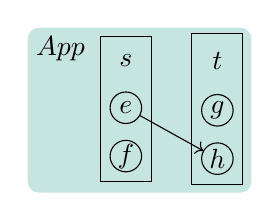
\begin{tikzpicture}
      \node[labeled] (App) {$App$};
      \service[right=of App.north, matrix anchor=north west]{s}{e,f}
      \service[right=of s]{t}{g,h}
      \begin{pgfonlayer}{background}
        \fill[app, fill=CbTeal, fill opacity=0.3]
        ([xshift=-1mm,yshift=1mm]App.north west)
        rectangle ([xshift=1mm, yshift=-1mm]t.south east);
      \end{pgfonlayer}
      % Workflow
      \draw [->] (s-2-1) -- (t-3-1);
    \end{tikzpicture}
    }
    \caption{Application $App$ made of two services $s$ and $t$ and
      four endpoints $e, f, g, h$. The $s.e \rightarrow t.h$
      represents an example of a workflow.}
    \label{fig:application}
  \end{subfigure}%\hfill%
  %% ~~~~~~~~~~~~~~~~~
  %% App instantiating
  \vspace{12pt}
  \begin{subfigure}[b]{.7\textwidth}
    \centering
    \scalebox{1.2}{
    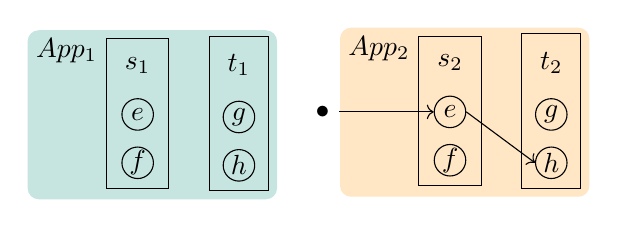
\begin{tikzpicture}
      % Instance A1
      \node[labeled] (App_1) {$App_1$};
      \service[right=of App_1.north, matrix anchor=north west]{s_1}{e,f}
      \service[right=of s_1]{t_1}{g,h}
      \begin{pgfonlayer}{background}
        \fill[app, fill=CbTeal, fill opacity=0.3]
        ([xshift=-1mm,yshift=1mm]App_1.north west)
        rectangle ([xshift=1mm, yshift=-1mm]t_1.south east);
      \end{pgfonlayer}

      % Instance A2
      \node[labeled, right=10mm of t_1.north east, anchor=north west] (App_2) {$App_2$};
      \service[right=of App_2.north, matrix anchor=north west]{s_2}{e,f}
      \service[right=of s_2]{t_2}{g,h}
      \begin{pgfonlayer}{background}
        \fill[app, fill=CbOrange, fill opacity=0.3]
        ([xshift=-1mm,yshift=1mm]App_2.north west)
        rectangle ([xshift=1mm, yshift=-1mm]t_2.south east);
      \end{pgfonlayer}

      % Workflow
      \node (c) [left=12mm of s_2-2-1] {$\bullet$};
      \draw [->] (c.east)      edge (s_2-2-1.west)
                 (s_2-2-1.east) -- (t_2-3-1.west);
    \end{tikzpicture}
    }
    \caption{Two independent instances $App_1$ and $App_2$ of the
      $App$ application. The $\bullet$ represents a client that
      executes the $s.e \rightarrow t.h$ workflow in $App_2$.}
    \label{fig:instances}
  \end{subfigure}
  \caption{Microservices architecture of a Cloud application}
  \label{fig:soa}
\end{figure}

\autoref{fig:soa} illustrates workflows in service-based applications.
%
%
On the top, \autoref{fig:application} represents a typical application
$App$ made of two services $s$, $t$ exposing endpoints $e$, $f$, $g$,
$h$.
%
It shows an example of a really simple workflow $s.e \rightarrow t.h$,
where a function in service $s$ calls an endpoint $h$ on service
$h$.
%
This is a figure similar to the~\autoref{fig:typical-app}
(page~\pageref{fig:typical-app}), but also exposing the endpoints.
%
% $App$ could be for example the OpenStack application.
% %
% In this context, service $s$ is the compute service that manages VMs.
% %
% Its endpoint $e$ creates VMs and $f$ lists them.
% %
% Service $t$ is the image service that controls operating system
% BLOBs.
% %
% Its endpoint $g$ stores an image and $h$ downloads one.
% %
% The composition $s.e \rightarrow t.h$ models the boot workflow (as
% seen in \autoref{fig:os}).
%%

On the bottom, \autoref{fig:instances} represents two application
instances of $App$ and their corresponding service instances: $s_1$
and $t_1$ for $App_1$; $s_2$ and $t_2$ for $App_2$.
%
A client ($\bullet$) triggers the execution of the workflow
$s.e \rightarrow t.h$ on $App_2$.
%
The request is addressed to the endpoint $e$ of $s_2$ which, in turn,
handles it and contacts the endpoint $h$ of $t_2$.
%
It is important to understand that it is the same exact workflow in
both figures; the second figure only have two instances of the same
application, and a client triggering the workflow
$s_2.e \rightarrow t_2.h$ on the second instance.


As discussed several times, running one instance of a microservices
application honors the local-first principle \emph{automatically} .
%
Since \autoref{fig:instances} shows two independent instances, they
could be deployed on two different sites, which would be a first step
towards a global infrastructure.
%
This is the configuration presented in \autoref{fig:soa-sites}, with a
request executed on $Site_2$, without impacting $Site_1$ at all.

\begin{figure}[htbp]
  \centering
    \scalebox{1.2}{
    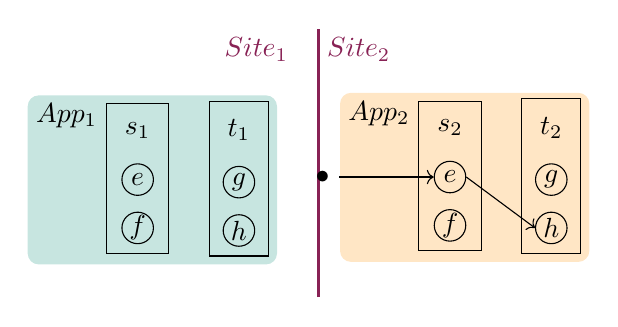
\begin{tikzpicture}
      % Instance A1
      \node[labeled] (App_1) {$App_1$};
      \service[right=of App_1.north, matrix anchor=north west]{s_1}{e,f}
      \service[right=of s_1]{t_1}{g,h}
      \begin{pgfonlayer}{background}
        \fill[app, fill=CbTeal, fill opacity=0.3]
        ([xshift=-1mm,yshift=1mm]App_1.north west)
        rectangle ([xshift=1mm, yshift=-1mm]t_1.south east);
      \end{pgfonlayer}

      % \node[labeled, left=20mm of t_1.north east, above=10mm of t_1.north east, anchor=north west] (Site_1) {$Site_2$};
      \node[labeled, text=CbPlum, xshift=20mm,yshift=10mm, anchor=north west] (Site_1) {$Site_1$};
      \node[labeled, text=CbPlum,xshift=33mm,yshift=10mm, anchor=north west] (Site_2) {$Site_2$};
      \draw [CbPlum!100, very thick] (3.2,-2.3)--(3.2,1.1);

      % Instance A2
      \node[labeled, right=10mm of t_1.north east, anchor=north west] (App_2) {$App_2$};
      \service[right=of App_2.north, matrix anchor=north west]{s_2}{e,f}
      \service[right=of s_2]{t_2}{g,h}
      \begin{pgfonlayer}{background}
        \fill[app, fill=CbOrange, fill opacity=0.3]
        ([xshift=-1mm,yshift=1mm]App_2.north west)
        rectangle ([xshift=1mm, yshift=-1mm]t_2.south east);
      \end{pgfonlayer}

      % Workflow
      \node (c) [left=12mm of s_2-2-1] {$\bullet$};
      \draw [->] (c.east)      edge (s_2-2-1.west)
                 (s_2-2-1.east) -- (t_2-3-1.west);
    \end{tikzpicture}
    }
  \caption{Two instances of a Cloud application on two different sites}
  \label{fig:soa-sites}
\end{figure}


%
Having entire independent instances on different sites means every
local requests can be executed on each site, even in case of network
partition.
%
However for the global system, it results in plenty of concurrent
values of the same resource distributed but isolated among all
instances (\eg two sites manage the same kind of resources but
their values differ as time passes).
%
With this configuration, manipulating any concurrent value on any
instance requires to code the collaboration in the application and let
clients specify how to use it.
%
Moreover, collaborations are required for a single coherent system, as
we discussed in~\autoref{chap:cloud-app-to-edge}.


Furthermore, as mentioned several times, the modular decomposition of
the code is popular for programmers of microservices architecture
because it divides the functionality of the application into
\emph{independent and interchangeable} services~\cite{Lis72}.
%
% This brings well-known benefits including ease of reasoning by
% decoupling the different concerns.
%
The most important benefit of this for us is exactly the modularity,
which gives the ability to \emph{change} a service with a defined API
by any service exposing the same API and logic~\cite{Par72}.
%
Thus, it allows the use of the same service located on another
site, or of another version of a service (newer or older), or the
same service in the same location but on a different server (for
load-balancing purposes), or even an entirely different service, as
long as all these services expose the same API and have the same
logic.

\begin{figure}[htbp]
  \centering
  \scalebox{1.2}{
    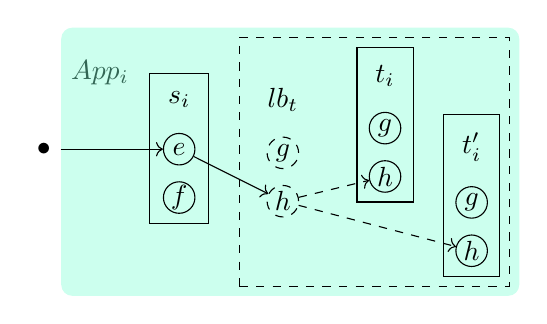
\begin{tikzpicture}
      % Service s
      \service{s_i}{e,f}

      % Service t
      \mesh[right=of s_i]{lb_t}{g,h}
      \service[right=5mm of lb_t, yshift=3mm]{t_i}{g,h}
      \service[right=16mm of lb_t, yshift=-6mm]{t_i'}{g,h}
      \node[draw,dashed,fit=(lb_t)(t_i)(t_i')] (lb_t_area) {};

      % Application
      \begin{pgfonlayer}{background}
        \node[labeled, left=2.5mm of s_i.north west] (App_i) {$App_i$};
        \node[app, fill=Aquamarine, opacity=0.4, fit=(App_i)(s_i)(lb_t_area)] (App_i_area) {};
      \end{pgfonlayer}

      % Workflow
      \node (c) [left=13mm of s_i-2-1] {$\bullet$};
      \draw [->]        (c)       edge (s_i-2-1)
                        (s_i-2-1) edge (lb_t-3-1);
      \draw [->,dashed] (lb_t-3-1) edge (t_i-3-1)
                        (lb_t-3-1) edge (t_i'-3-1);
  \end{tikzpicture}}
  \caption{Load balancing principle}
  \label{fig:sm-loadbalance}
\end{figure}

For example, a load balancer makes good use of this property to
distribute the load between multiple instances of the same modular
service~\cite{Fie00}.
%
\autoref{fig:sm-loadbalance} shows this process with a reverse proxy
for load balancing $lb_t$ of the service $t$.
%
In the figure, $lb_t$ intercepts and balances incoming requests
within two service instances $t_i$ and $t_i'$ during the execution of
the workflow $s.e \rightarrow t.h$ in $App_i$.
%
From one execution to another, the endpoint $s_i.e$ gets result from
$t_i.h$ or $t_i'.h$ in a safe and transparent manner thanks to the
modularity.


\begin{tcolorbox}[colframe=CbTeal,colback=CbCyan]
\textbf{Thus, we can redirect a request to another instance of the
  same service.}
\end{tcolorbox}




As microservices architectures are the foundations of \gls{DevOps}
practices, because their modular decomposition of services allows for
their independent instantiation and maintenance.
%
As discussed in~\autoref{chap:soa-SM}, a service mesh takes benefit
from this decomposition/modularity to implement communication-derived
features such as monitoring, message routing or load balancing outside
of the application.
%%
In its most basic form, a service mesh consists in a set of reverse
proxies around service instances, each proxy encapsulating a
specific code to control communications between
services~\cite{LLGZG19}.
%
This encapsulation in each proxy \emph{decouples} the code managed by
\gls{DevOps} for their infrastructure deployment from the application
business logic maintained by programmers.
%
It also makes the service mesh \emph{generic} to all services by
considering them as black boxes and only taking into account their
communication requests.

\begin{figure}[htbp]
  \centering
  \scalebox{1.25}{
  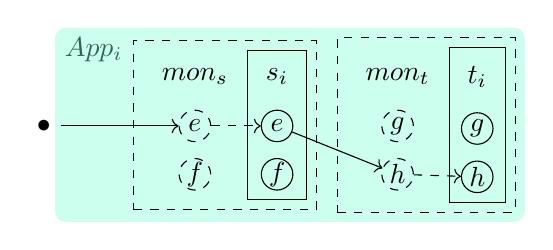
\begin{tikzpicture}
    % Service s
    \mesh{mon_s}{e,f}
    \service[right=0mm of mon_s]{s_i}{e,f}
    \node[draw,dashed,fit=(mon_s)(s_i)] (mon_s_area) {};

    % Service t
    \mesh[right=of s_i]{mon_t}{g,h}
    \service[right=0mm of mon_t]{t_i}{g,h}
    \node[draw,dashed,fit=(mon_t)(t_i)] (mon_t_area) {};

    % Application
    \begin{pgfonlayer}{background}
      \node[labeled, left=2.5mm of mon_s.north west] (App_i) {$App_i$};
      \node[app, fill=Aquamarine, opacity=0.4, fit=(App_i)(mon_s_area)(mon_t_area)] (App_i_area) {};
    \end{pgfonlayer}

    % Workflow
    \node (c) [left=15mm of mon_s-2-1] {$\bullet$};
    \draw [->]        (c)         edge (mon_s-2-1);
    \draw [->,dashed] (mon_s-2-1) edge (s_i-2-1);
    \draw [->]        (s_i-2-1)   edge (mon_t-3-1);
    \draw [->,dashed] (mon_t-3-1) edge (t_i-3-1);
  \end{tikzpicture}
}
  \caption{Service mesh $mon$ for the monitoring of requests}
  \label{fig:servicemesh}
\end{figure}


\autoref{fig:servicemesh} illustrates a service mesh monitoring
requests to have insight about the application.
%
The reverse proxies $\mathit{mon_s}$ and $\mathit{mon_t}$ collect
metrics on requests directed to service instances respectively $s_i$
and $t_i$, in this case, during the execution of the workflow
$s.e \rightarrow t.h$ on $App_i$.
%
They are illustrated as dashed rectangles around the services and a
mimic of the endpoints present in the services.
%
The encapsulated code in $\mathit{mon_s}$ and $\mathit{mon_t}$
collects for example requests latency and success/error rates.
%
It may send metrics to a time series database as
InfluxDB~\cite{influxdb} and could be changed by anything else without
touching any of the $\mathit{App}$ application code.


The collaborations we need between multiple instances of an
application can actually be done by using a service mesh on the
infrastructure and programming redirections of the workflow.
%
Indeed, a service mesh could allow dynamic composition of services on
different sites.
%
And because a service mesh is generic, it can be extended to all
applications built by service composition.

\begin{tcolorbox}[colframe=CbTeal,colback=CbCyan]
\textbf{At this point, with the modularity of services and the service
  mesh logic, we have the ability to use another instance of a service
  and a way to do it easily and dynamically.}
\end{tcolorbox}

To program dynamically the collaborations, we developed a domain
specific language called \emph{\scl}.


\section{Scope-Lang, a DSL to reify locations and collaborations of
  requests}
\label{sec:scl}

%Generic collaboration via dynamic composition.


To define dynamically how a particular request should be handled by
the service mesh, we developed a Domain Specific Language
(\acrshort{DSL}) that extends the default API with location
information.
%
Entitled \scl, it enables users to specify, for each resource, in
which context the execution should take place.
%

Scope-lang extends the way clients and users interact with the services,
whether it is through command lines or through a REST API.
%
Because we were originally working on \os, the \scl was designed to be
added at the end of command lines; but it could obviously be included
in a HTTP request, like in the header.

%
A \scl expression (referred to as the \emph{scope} or $\sigma$
in~\autoref{fig:scl}) contains location information that defines, for
each service involved in a workflow, in which instance the execution
takes place.
%
To put it simply: considering the previous application, the scope
``$\mathit{s: App_1, t : App_2}$'' intuitively tells to use the
service $s$ from $App_1$ and $t$ from $App_2$.
%
Conversely, the scope ``$\mathit{t: App_1 \& App_2}$'' specifies to
use the service $t$ from $\mathit{App_1}$ and $\mathit{App_2}$.


  %% ~~~~~~~~~~~~~~~~~
  %% Scope lang expressions
\begin{figure}[hbtp]%{.6\textwidth}
  \centering
  \footnotesize
  \[\begin{array}{l c l l}
      App_i,App_j  &::=  &\multicolumn{2}{l}{\text{application instance}}\\
      s,t          &::=  &\multicolumn{2}{l}{\text{service}}\\
      s_i,t_j      &::=  &\multicolumn{2}{l}{\text{service instance}}\\
      Loc      &::=  &App_i           &\enspace\text{single location}\\
                   &\mid &Loc \& Loc      &\enspace\text{multiple locations}\\
                   &\mid & Loc \% Loc     &\enspace\text{cross locations}\\
                   %% &\mid &Loc ; Loc       \\
        \sigma   &::=  &s: Loc, \sigma  &\enspace\text{scope}\\
                 &\mid &s: Loc
      \end{array}\]
    \vspace{-5pt}
    \begin{align*}
    \mathcal{R}[\![ s : App_i ]\!]        &= s_i \\
    \mathcal{R}[\![ s : Loc \& Loc' ]\!]  &= \mathcal{R}[\![ s : Loc ]\!]  \text{ and }
                                            \mathcal{R}[\![ s : Loc' ]\!] \\
    \mathcal{R}[\![ s : Loc \% Loc' ]\!]  &= \mathcal{R}[\![ s : Loc ]\!]  \text{ spread to }  \mathcal{R}[\![ s : Loc' ]\!]
    \end{align*}

    \vspace{-5pt}
    \caption{\scl expressions $\sigma$ and the function that resolves
      service instance from elements of the scope $\mathcal{R}$.}
    \label{fig:scl}
    %% \mathcal{R}[\![ s : Loc ; Loc' ]\!]  &= \\
    %%   \mathcal{R}[\![ s : Loc ]\!] &\text{ otherwise } \mathcal{R}[\![ s : Loc' ]\!]
\end{figure}


\autoref{fig:scl} presents the logic of \scl as a grammar and the
function $\mathcal{R}$ that resolves the workflow induced by the given
scope.
%
We will discuss later (\autoref{sec:collaborations}) the different
opportunities of collaborations offered by \scl.
%
For now, we will mention only that the comma ``$,$'' represents the
\emph{sharing} collaboration; the ampersand ``$\&$'' represents the
\emph{replication} collaboration; and the percent ``$\%$'' represents
the \emph{cross} collaboration.
%
These are the three main types of collaborations we envisioned, with
more operators that could be defined for more flexibility in the
requests.


%% Geo-distributing service mesh
\begin{figure}[h!]%{.8\textwidth}
  \centering
  \scalebox{1.3}{
    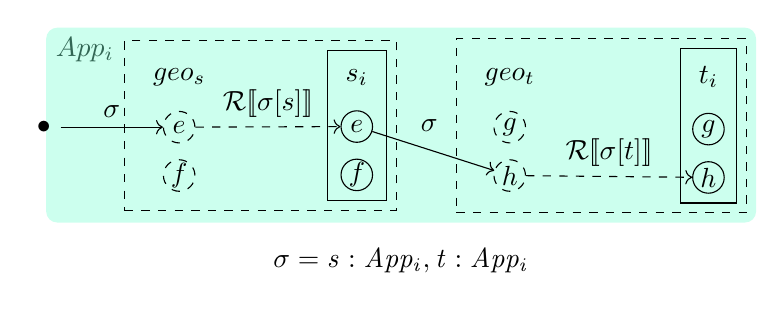
\begin{tikzpicture}
      % Service s
      \mesh{geo_s}{e,f}
      \service[right=13mm of geo_s]{s_i}{e,f}
      \node[draw,dashed,fit=(geo_s)(s_i)] (geo_s_area) {};

      % Service t
      \mesh[right=10mm of s_i]{geo_t}{g,h}
      \service[right=16mm of geo_t]{t_i}{g,h}
      \node[draw,dashed,fit=(geo_t)(t_i)] (geo_t_area) {};

      \begin{pgfonlayer}{background}
        \node[labeled, left=2.5mm of geo_s.north west] (App_i) {$App_i$};
        \node[app, fill=Aquamarine, opacity=0.4, fit=(App_i)(geo_s_area)(geo_t_area)] (App_i_area) {};
      \end{pgfonlayer}

      % Workflow
      \node [below=2mm of App_i_area] {$\sigma = \mathit{s: App_i, t: App_i}$};
      \node (c) [left=13mm of geo_s-2-1] {$\bullet$};
      \draw [->]        (c)         -- node [auto] {$\sigma$} (geo_s-2-1);
      \draw [->,dashed] (geo_s-2-1) -- node [auto] {$\mathcal{R}[\![ \sigma[s] ]\!]$}
      (s_i-2-1);
      \draw [->]        (s_i-2-1)   -- node [midway,xshift=-.5mm,label={$\sigma$}] {} (geo_t-3-1);
      \draw [->,dashed] (geo_t-3-1) -- node [auto] {$\mathcal{R}[\![ \sigma[t] ]\!]$}
      (t_i-3-1);
    \end{tikzpicture}
  }
  \caption{Scope $\sigma$ interpreted by the geo\hyph{}distribution
    service mesh $geo$ during the execution of the $s.e
    \xrightarrow{\sigma} t.h$ workflow in $App_i$. Reverse proxies
    perform requests forwarding based on the scope and the
    $\mathcal{R}$ function.}
  \label{fig:sm-geo}
\end{figure}


Clients set the scope of a request to also specify the collaboration
between instances they want for a specific execution.
%
The scope is then \emph{interpreted} by our service mesh during the
execution of the workflow to fulfill that collaboration.
%
The main operation it performs is \emph{request forwarding}.
%

\autoref{fig:sm-geo} presents, as before, an application $App_i$ with
two services $s_i$ and $t_i$, but this time they are encapsulated,
behind proxies.
% that intercept the requests and execute them according to the defined scope.
%
These proxies in front of service instances ($\mathit{geo_s}$ and
$\mathit{geo_t}$ in \autoref{fig:sm-geo}) the requests and execute
them according to the defined scope.
%
``Where'' the requests will be executed exactly depends on locations
in the scope.
%



The interpretation of the scope always follow these steps:
\begin{enumerate}
\item
  A request is sent to the endpoint of a service of one
  application instance.  The request piggybacks a scope, typically as
  an HTTP header in a RESTful application. For example in
  \autoref{fig:sm-geo}: \smash{$\bullet \xrightarrow{\mathit{s:
        App_i, t: App_i}} s.e$}.

\item
  The reverse proxy in front of the service instance intercepts the
  request and reads the scope. In \autoref{fig:sm-geo}: $geo_s$
  intercepts the request and reads $\sigma$ which is equal to
  $\mathit{s: App_i, t: App_i}$.

\item
  The reverse proxy extracts the location assigned to its service from
  the scope.  In \autoref{fig:sm-geo}: $geo_s$ extracts the location
  assigned to $s$ from $\sigma$. This operation, noted $\sigma[s]$,
  returns $\mathit{App_i}$.

\item
  The reverse proxy uses a specific function $\mathcal{R}$ (see
  \autoref{fig:scl}) to resolve the service instance at the assigned
  location.  $\mathcal{R}$ uses an internal registry.  Building the
  registry is a common pattern in service mesh using a \emph{service
  discovery}~\cite{LLGZG19} and therefore is not presented here.  In
  \autoref{fig:sm-geo}: $\mathcal{R}[\![ s: \sigma[s] ]\!]$ reduces to
  $\mathcal{R}[\![ \mathit{s : App_i} ]\!]$ and is resolved to service
  instance $s_i$.
\item
  The reverse proxy \emph{forwards} the request to the endpoint of the
  resolved service instance. In \autoref{fig:sm-geo}: $geo_s$ forwards
  the request to $s_i.e$.
\end{enumerate}



In this example of executing the workflow $s.e \xrightarrow{\sigma}
t.h$, the endpoint $s_i.e$ has in turn to contact the endpoint $h$
of service $t$.
%
The reverse proxy $geo_s$ propagates the scope on the
outgoing request towards the service $t$.
%
The request then goes through stages 2 to 5 on behalf of the reverse
proxy $geo_t$.
%
It results in a forwarding to the endpoint
$\mathcal{R}[\![ t: \sigma[t] ]\!].h$ that is resolved to $t_i.h$.
%
Here, the scope only refers to one location (\ie $\mathit{App_i}$).
%
Thus the execution of the workflow remains \emph{local} to that
location.
%
The next section details the use of forwarding in order to
perform collaborations between instances.




\section{What kind of collaborations do we need?}
\label{sec:collaborations}



Previously, we presented how a load balancer changes the composition
between multiple instances of the same service \emph{inside} a single
application instance.
%
In contrast, in the previous example for \scl, we change the
composition between multiple instances of the same service
\emph{across} application instances.
%
As a consequence, these different service instances on different sites
can share their resources during the execution of a workflow.

This is done only by redirecting requests to other application
instances, located on other sites.
%
We call this mechanism \emph{forwarding}, and it is the basis of all
the possible collaborations.
%
We will now see different collaborations envisioned, of which the
first three are essential to provide a single coherent system
(sharing, replication, cross, mentioned before in \autoref{sec:scl}), and the others only
adding some possibilities for the users.

% \textbf{We generalize this mechanism to share resources}.
%

%

\subsection{Forwarding for resource sharing}
\label{ssec:scl-share}


\autoref{fig:sharing} depicts the dynamic composition mechanism
described above during the execution of the workflow
\smash{$s.e \xrightarrow{\mathit{s: App_1, t: App_2}} t.h$}.
%
The service instance $s_1$ of $App_1$ is dynamically composed thanks
to the forwarding operation of the service mesh with the service
instance $t_2$ of $App_2$.
%
This forwarding is safely relying on the guaranty provided by
modularity: if $t$ is modular, then we can swap $t_1$ by $t_2$ since
they have the same API and logic, as they are different instances of
the same service.
%
This implies obviously that they have to be the same major version to
present the same API.
%


\begin{figure}[htbp]
  \centering
  \scalebox{1}{
  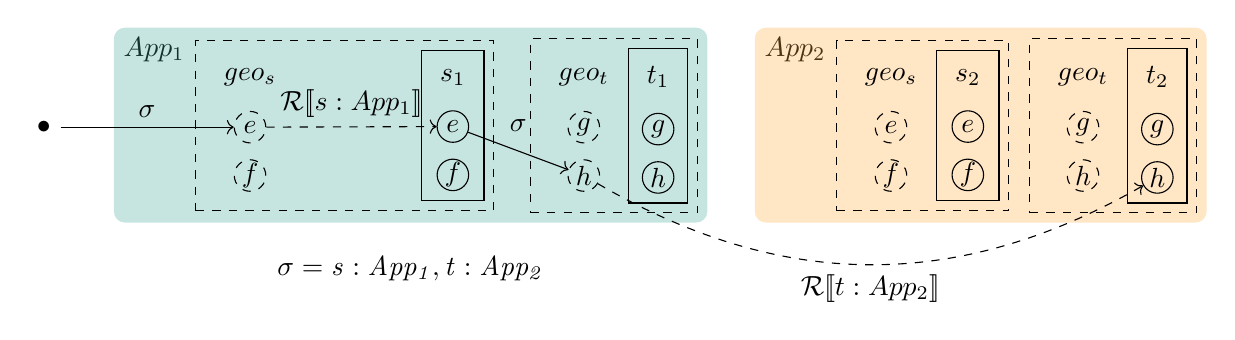
\begin{tikzpicture}
    % Instance App_1
    \mesh{geo_s}{e,f}
    \service[right=16mm of geo_s]{s_1}{e,f}
    \node[draw,dashed,fit=(geo_s)(s_1)] (geo_s_area) {};
    \mesh[right=7mm of s_1]{geo_t}{g,h}
    \service[right=0mm of geo_t]{t_1}{g,h}
    \node[draw,dashed,fit=(geo_t)(t_1)] (geo_t_area) {};

    \begin{pgfonlayer}{background}
      \node[labeled, left=2.5mm of geo_s.north west] (App_1) {$App_1$};
      \node[app, fill=CbTeal, opacity=0.3, fit=(App_1)(geo_s_area)(geo_t_area)] (App_1_area) {};
    \end{pgfonlayer}

    % Instance App_2
    \idmesh[right=20mm of t_1]{geo_s'}{geo_s}{e,f}
    \service[right=0mm of geo_s']{s_2}{e,f}
    \node[draw,dashed,fit=(geo_s')(s_2)] (geo_s'_area) {};
    \idmesh[right=of s_2]{geo_t'}{geo_t}{g,h}
    \service[right=0mm of geo_t']{t_2}{g,h}
    \node[draw,dashed,fit=(geo_t')(t_2)] (geo_t'_area) {};

    \begin{pgfonlayer}{background}
      \node[labeled, left=2.5mm of geo_s'.north west] (App_2) {$App_2$};
      \node[app, fill=CbOrange, opacity=0.3, fit=(App_2)(geo_s'_area)(geo_t'_area)] (App_2_area) {};
    \end{pgfonlayer}

    \node [below=3mm of App_1_area] {$\sigma =\mathit{s: App_1, t: App_2}$};

    % Workflow
    \node (c) [left=22mm of geo_s-2-1] {$\bullet$};
    \draw [->]  (c) -- node [auto] {$\sigma$} (geo_s-2-1);
    \draw [->,dashed] (geo_s-2-1) --
      node [auto] {$\mathcal{R}[\![ s : App_1 ]\!]$}
      (s_1-2-1);
    \draw [->]        (s_1-2-1) -- (geo_t-3-1)
      node [midway, label={$\sigma$}] {};
    \draw [->,dashed] (geo_t-3-1) edge [bend right]
      node [below] {$\mathcal{R}[\![ t : App_2 ]\!]$} (t_2-3-1);
    %% \draw [->,dashed] (geo_t'-3-1) -- (t_2-3-1)
    %%   node [midway, label=above:{$\mathcal{R}[\![ t : App_2 ]\!]$}] {};
  \end{tikzpicture}
  }
  \caption{Resource sharing by forwarding between instances}
  \label{fig:sharing}
\end{figure}

The process is similar to the one described in~\autoref{sec:scl}, but
with $\mathit{s: App_1, t: App_2}$, resulting in a forwarding to the
endpoint $\mathcal{R}[\![ t: \sigma[t] ]\!].h$ that is resolved to
$t_2.h$, with $t_2$ the $t_i$ service instantiation in $App_2$.
%
Since it is so similar, we avoid repeating it further.
%
As a result of this request, the endpoint $s_1.e$ benefits from
resource values of $t_2.h$ instead of its usual $t_1.h$.
%

This is the collaboration we call \emph{resource sharing}, or shorter
\emph{sharing}.


\subsection{Forwarding for resource replication}
\label{ssec:scl-rep}

%% To ease the explanation in the following,
Replication is the ability to create and maintain identical resources
on different sites: an operation on one replica should be propagated to
the other ones according to a certain consistency policy.
%
In our context, it is used to deal with latency and availability.


Microservices often follow a RESTful HTTP API and so generate an
identifier for each resource.
%
This identifier is later used to retrieve, update or delete resources.
%
In our approach, each application instance is independent.
%
Therefore, it requires a meta-identifier so users can manipulate
replicas across the different sites as a unique resource and to unify
these identifiers.
%
Furthermore, we need to associate this meta-identifier to local
identifiers for each involved site.
%
To do so, we propose a mapping
$\{ metaId: [App_i: localID_i], service\_name\}$ to keep track of
replicated resources and apply further changes to all replicas.
%
The service name will be used locally by the registry of the service
mesh to find which service to contact.

\begin{figure}[htbp]
  \centering
  \scalebox{1.23}{
  \begin{tikzpicture}
    % Instance App_1
    \mesh{geo_t}{g,h}
    \service[right=20mm of geo_t]{t_1}{g,h}
    \node[draw,dashed,fit=(geo_t)(t_1)] (geo_t_area) {};
    \node[db, below=of geo_t, xshift=-10mm, aspect=0.25](db_1){};

    \begin{pgfonlayer}{background}
      \node[labeled, left=2.5mm of geo_t.north west] (App_1) {$App_1$};
      \node[app, fill=CbTeal, opacity=0.3, fit=(App_1)(db_1)(geo_t_area)] (App_1_area) {};
    \end{pgfonlayer}

    % Instance App_2
    \idmesh[right=30mm of t_1]{geo_t'}{geo_t}{g,h}
    \service[right=10mm of geo_t']{t_2}{g,h}
    \node[draw,dashed,fit=(geo_t')(t_2)] (geo_t'_area) {};
    \node[db, below=of geo_t', xshift=0mm, aspect=0.25](db_2){};

    \begin{pgfonlayer}{background}
      \node[labeled, left=2.5mm of geo_t'.north west] (App_2) {$App_2$};
      \node[app, fill=CbOrange, opacity=0.3, fit=(App_2)(db_2)(geo_t'_area)] (App_2_area) {};
    \end{pgfonlayer}

    \node [below=1mm of App_1_area] {$\sigma =\mathit{t: App_1 \& App_2}$};

    % Workflow
    \node (c) [left=20mm of geo_t-2-1] {$\bullet$};
    \draw [->]  (c) -- node [auto] {$\sigma$} (geo_t-2-1);
    \draw [->,dashed] (geo_t-2-1) --
    node [auto] {$\mathcal{R}[\![ t : App_1 ]\!]$}
    (t_1-2-1);
    \draw [->, dashed] (geo_t-2-1) edge [bend right]
    node [below, xshift=4mm, label={$\mathcal{R}[\![ t : App_2 ]\!]$}] {}
    (t_2-2-1);
    \draw [->,dashed] (geo_t-2-1) edge [bend right] (db_1);
    \draw [->,dashed] (geo_t-2-1) edge [bend right] (db_2);
  \end{tikzpicture}
  }
  \caption{Replication by forwarding on multiple instances}
  \label{fig:replication}
\end{figure}

For example, in \autoref{fig:replication}, the service $t$
exposes an endpoint $g$ that creates a resource.
%
When using a scope to create replicas of the same resource, such as
$t: \mathit{App_1 \& App_2}$, the service mesh generates a
meta-identifier and maps it
$\{ metaId: [App_1: localID_{t_1}, App_2: localID_{t_2}], t\}$.
%
If $t_1$ creates a replica of the resource with the identifier 42 and
$t_2$ with the identifier 6, and our meta-identifier was generated as
72, the mapping is: \{$72: [App_1: 42, App_2: 6], t$\}.
%
These mappings are stored in an independent database alongside each
application instance, in the control plane
(see~\autoref{chap:soa-SM},~\autoref{fig:sm-arch} for a reminder on
the control plane of a service mesh).


The replication process follows these steps:
\begin{enumerate}
\item
  A request for replication is addressed to the endpoint of a
  service of one application instance.  For example in
  \autoref{fig:replication}: \smash{$\bullet \xrightarrow{t: App_1\&App_2}
  t.g$}.

\item
  Similarly to the sharing, the $\mathcal{R}$ function is used to
  resolve the endpoints that will store replicas. $\mathcal{R}[\![ s :
      Loc \& Loc' ]\!] = \mathcal{R}[\![ s : Loc ]\!]  \text{ and }
  \mathcal{R}[\![ s : Loc' ]\!]$. In our example:
  $\mathcal{R}[\![ t : App_1 \& App_2 ]\!]$ is equivalent to
  $\mathcal{R}[\![ t : App_1 ]\!]  \text{ and } \mathcal{R}[\![ t :
      App_2 ]\!]$. Consequently, $t_1$ and $t_2$.

\item
  The meta-identifier is generated along with the mapping and
  added in the database. In \autoref{fig:replication}: \{ $ 72:
  [App_1: \mathit{none}, App_2: \mathit{none}], t$\}.

\item
  Each request is forwarded to the corresponding endpoints on involved
  sites and a copy of the mapping is stored in those sites' database
  simultaneously. In \autoref{fig:replication}: $geo_t$ forwards the request to
  $t_1.g$ and $t_2.g$ and stores the mapping $\{72: [App_1:
    \mathit{none}, App_2: \mathit{none}], t\}$ in $App_1$ and $App_2$
  databases.

\item
  Each contacted service instance executes the request and returns the
  results (including the local identifier) to the service mesh.  In
  \autoref{fig:replication}: $t_1$ and $t_2$ returns respectively the
  local identifier $42$ and $6$.

\item
  The service mesh completes the mapping and populates the involved
  sites' databases. In \autoref{fig:replication}: the mapping now is
  $\{72: [App_1: 6, App_2: 42], t\}$ and added to databases on $App_1$
  and $App_2$ sites.

\item
  By default, the meta identifier is returned as the final response.
  If a response other than an identifier is expected, the first
  received response is transferred (since others are replicas with
  similar values).
\end{enumerate}


This process ensures that only interactions with the involved sites
occur, avoiding wasteful communications.
%
Each operation that would later modify or delete one of the replicas
will be applied to every other using the mapping available on each
site.
%
To prevent any direct manipulation that would break the consistency,
either local identifiers of replicas can be hidden to the users or
each operations executed need to check in the database if the local
identifier exist in a mapping, but it is really slower.
%
Another way is to warn users from the beginning that if they
manipulate replicated resources through their local identifiers, no
guarantees can be offered on the consistency.


This replication control perfectly suits our collaborative-then
principle.
%
It allows a client to choose ``when'' and ``where'' to replicate.
%
Regarding the ``how'', our current process for forwarding replica
requests, maintaining mappings and ensuring that operations done on
one replica are applied on others, is naive.
%
Implementing advanced strategies is left for the implementation.
%
However, we underline that it does not change the foundations of our
proposal.
%
Ultimately, choosing the strategy should be made possible at the \scl
level (\eg weak, eventual or strong consistency), through different
operators, for example.


Finally, to conclude on the approach of the different collaborations
and the scope, we have to add that in the absence of a scope for an
execution, every operation in the workflow will be local to where the
request was made.
%
Moreover, if all the involved services are not specified in the scope,
because a lot of services can be involved in a single workflow, the
execution will be local to where the request is currently located.
%
This keeps the approach local-first as much as possible.





\subsection{Forwarding for cross}
\label{ssec:scl-cross}

This last collaboration is the less mature one and another PhD
candidate, Geo Johns Antony is working currently on it specifically.


\emph{Cross} is inspired from an early study that focused on extending
virtual networks between multiple Edge sites~\cite{ELNC20}.
%
The idea is to create a resource over multiple sites.
%
The main difference to the aforementioned replication collaboration is
related to the aggregation/divisibility property.
%
% In the replication, each copy is independent, even if they all
% converge eventually based on the CRUD operation.
%
A cross resource can be seen as an aggregation of all resources or
part of resources that constitutes the cross-resource overall.
%
Some resources which cannot be divided by an application API will
require an additional layer in the business logic to satisfy the
divisibility property.
%\todo{Add one sentence that explains that it requires dedidacted code that goes beyond the existing vanilla code. (example namespace: no code, but pods: code.}


Cross thus revolves around two properties:
  \begin{description}
  \item{\textbf{Aggregation}} This property aggregates the resources from
    various involved geo-distributed sites.
  %
  This property is maintained at each of these locations.
  %
  Cross is aware about each involved site.
  %
  It provides the illusion of a single site for resources which are
  geo-distributed across sites.
  %
  Users instantiate the request with \scl and Cross aggregates this
  request to give results from multiple geo-distributed sites.
\item{\textbf{Divisibility}} Cross divides the resources into various
  geo-distributed locations.
  %
  While creating a resource, if the resource is further divisible by
  the application API, cross manages to divide the resource into
  further smaller resources.
  %
  While dividing, cross creates a prime site, which will be the site
  of the location in the request and other sites get an illusion of
  the resource from this site.
  %
  For each resource, the prime site may be different, as it is defined
  per resource by the users.
  % based on the scope
  % given by users.
  % For each resource, the prime site may be different based on the
  % scope given by the users.
\end{description}


A \texttt{CREATE} operation for instance can distribute the resource
over different sites (if this resource is divisible), while a
\texttt{GET} will be performed on each ''sub-resource'' composing the
cross-resource in order to return the aggregated result.
%
Similarly to the replicant data scheme, the different resources
involved are monitored in order to perform CRUD operations in the
expected manner.
%

The illusion of single-site is created with two primary principles.
%
At each location, all the resources are available and extended.
%
Any CRUD operations can be performed at any of the sites specified
with the scope and applied to the entire Cross resource.
%
The interaction will be similar to performing a request local to the
application.
%
The communication layer created by our generic solution ensures the
transfer of request across each site.
%

How we deal with the split brain issue for cross-resource is left
as future work.
%
However, it is worth noting that the unreachability of one site that
hosts a part of the cross-resource faces multiple challenges.
%
These challenges are currently addressed by Geo Johns Antony, in his
own PhD thesis.




\subsection{More (and more about) collaborations} % 2p
% \addcontentsline{toc}{section}{More collaborations}
\label{ssec:more-collabs}

We discussed in this manuscript about three collaborations, namely,
sharing, replication and cross.
%
But to fit perfectly to the needs of the users, we can also envision
more types of collaborations and operators.
%
The reflection presented in this section has been presented in our
Euro-Par paper~\cite{CDL21}.

The code of \scl is independent of cloud applications and can easily
be extended with new features in it.
%
Scope-lang is thus a great way to implement additional operators to
give more control during the manipulation of resources, although it
has been initially designed for resources sharing and replication, and
then cross.
%
Choosing between different levels of consistency in the replication is
one example of possible new operators.
%
For some resources, applications can require stronger or weaker
consistencies, depending on what is done with these resources.
%
Each consistency could co-exist with different logics and operators
according to the resources requirements.
%
This would allow the users to define what type of consistency they
need for different resources, and thus for example when operations
should be fast and when they can be slow to improve consistency, such
as a RedBlue consistency~\cite{LPCG+12}.

%
In this section, I present two other operators to stress the
generality of the approach regarding possible operations, namely the
\emph{otherwise} operator and the one derived from it, the \emph{around} operator.


\subsubsection{Otherwise}

The new \emph{otherwise} operator (``$Loc_1;Loc_2$'' in
\autoref{fig:scl++}) informally tells to use the first location or
fallback on the second one if there is a problem.
%
This operator comes in handy when a client wants to deal with sites
disconnections.
%
Adding it to the service mesh implies to implement in the Cheops core
what to do when it interprets a scope with a ($;$).
%
The implementation is straightforward: make the service mesh forward
the request to the first location and proceed if it succeeds, or
forward the request to the second location otherwise (if it fails for
any reason).
\begin{figure}[htbp]
  \centering
  %% ~~~~~~~~~~~~~~~~~
  %% Scope lang expressions
    \small
    \[\begin{array}{l c l l}
    Loc      &::=  &\dots      &\enspace(\text{see \autoref{fig:scl} for \dots})\\
    &\mid &Loc ; Loc  &\enspace\text{otherwise location}
    \end{array}\]
    $\mathcal{R}[\![ s : Loc_1 ; Loc_2 ]\!]  =
    \mathcal{R}[\![ s : Loc_1 ]\!]  \text{ otherwise }
     \mathcal{R}[\![ s : Loc_2 ]\!]$
    \caption{The otherwise ($;$) operator.  }
    \label{fig:scl++}
  \end{figure}
  %% ~~~~~~~~~~~~~~

\subsubsection{Around}
Ultimately, we can built new operators upon existing ones.
%
This is the case of the \texttt{around} function that considers all
locations reachable in a certain amount of time, \eg
\texttt{around($App_1$, 10ms)}.
%
To achieve this, the function combines the available locations with
the otherwise operator ($;$), as shown in \autoref{lst:around}.
%
This is made possible through the heartbeats between different
instances of Cheops that also retrieve the latency between the sites.
%
Thus it does not require to change the code of the interpreter in the
service mesh, only a small addition (presented
in~\autoref{lst:around}).

  %% Geo-distributing service mesh
  \begin{figure}[htbp]
    \centering
    \vspace{10pt}
    \begin{lstlisting}
def around(loc: Loc, radius: timedelta) -> Loc:
  # Find all Locs in the `radius` of `loc`
  # >  locs = [App1, App2, ..., Appn]
  locs = _find_locs(loc, radius)

  # Combine all `locs` with `;`
  # >  App1;App2;...;Appn
  return foldl(;, locs, loc)
    \end{lstlisting}
    \caption{The \texttt{around} operator build upon ($;$).}
    \label{lst:around}
\end{figure}


\subsubsection{Compositions of collaborations}
Another element we did not discuss entirely in this manuscript is
\emph{the composition of collaborations}.
%
If we consider for example, as suggested in the classification
thereafter (\autoref{sec:classification}), the replication of a
resource using a sub-resource on one site, we combine replication and
sharing.
%
Such a request would follow a command such as, for the creation of two
replicas of a resource $a$ on $Site_1$ and $Site_2$, with a
sub-resource from $Site_1$:
\begin{lstlisting}[numbers=none]
application create a --name bar --sub-resource foo \
           --scope{Service A: Site_1 & Site_2, Service B: Site_1}
\end{lstlisting}
% \noindent{\small\texttt{application create a -{}-name bar -{}-scope \{Service A:
% $Site_1$ \& $Site_2$\}}.}
Except for the dealing of dependencies (it would be probably better to
replicate also the sub-resource, if they are linked by reliance), this
is pretty straightforward.
%
This composition should be done in one step, as opposed to the one for
reliance, where the users would first need to replicate the
sub-resource ($foo$) before using it for the creation of $bar$ replicas
(and avoid using sharing).
%

Some compositions can be more tricky even.
%
What happens when users want to create a sub-resource inside a cross
resource which will not allow the name of the replicas to co-exist, as
the creation of pods through replication inside a cross namespace that
exist on several sites on Kubernetes?
%
The namespace spans on different sites, and we want to create a pod
$foo$, replicated of those different sites.
%
Unfortunately, the namespace will not accept the local creation
requests of $foo$, as the name will exist after the first request.
%
The problem with that is that it is not really a replication problem,
because replication will only execute the request without the scope
locally on each sites, and it is not exactly a cross problem, as
Kubernetes manage replicaset by giving replicas unique names.

%
This means that we need dedicated code to manage the composition of
collaborations, mainly because of the dependencies.



\section{Classification of resources dependencies} % 4p
\label{sec:classification}
%\addcontentsline{toc}{section}{Classification}

The classification of resources dependencies is a joint, on-going work
with Geo Johns Antony, who defined a draft model which was then
refined together, and adapted for our own collaborations.
%
This has been presented in our ICSOC 2022 paper~\cite{DAL22true,
  DAL22}.
%
Also, once again, the focus is made on the replication, but there
is similar work for cross.

Many resources have dependencies on each other (a virtual machine in
the OpenStack ecosystem depends on an image, a network, an IP, etc.; a
deployment file in Kubernetes is linked to several pods; etc.).
%
In fact, the sharing collaboration implies there is some kind of
dependency between the involved resources.
%
Hence, it is mandatory to rely on a relationship model for replication
and cross operations.
%
This model will be used to keep track on each critical resource and
ensure that CRUD operations are performed thoroughly.

%
We have identified and formulated three types of dependencies, depicted in
\autoref{fig:dependencies}.
\begin{figure}[htbp]
    \centering
    
\includegraphics[width=0.7\textwidth]{figs/pdf/classification.pdf}
    \caption{The different dependencies}
    \label{fig:dependencies}
  \end{figure}



\subsubsection{Requirement}

Requirement defines a relationship between two resources that is not
critical for the survival of either of the resource but rather is a
necessary link during a particular operation.
%
The operation can be any operation performed upon either of the
resource.
%
While performing the operation the link is vital and if the link is
severed the resultant operation will terminate and it will not
succeed.
%
If the link is maintained and no external factors affect the
operation, the operation will be a success and after this the link
between these resources is insignificant.
%
Hence, a broken link after the operation does not affect either of the
resource. An example for \os is a VM requires an image, for the
creation operation.

\vspace{-15pt}
\subsubsection{Reliance}

Reliance defines a relationship between two resources that is critical
for the survival of either one of the resource or both.
%
If the link between these resources is cut at some point during the
lifetime of these resources it will impact the existence of the
resources and can lead to a failure condition.
%
Involved resources are independent and one resource cannot alter the
other resource.
%
For example, in \ks, a pod, when created with a secret, relies on this
secret.

\vspace{-15pt}
\subsubsection{Composition}
Composition consists of intrinsic dependencies between resources: the
life cycle of the two resources are linked.
%
The creation of resource A implies the creation (and respectively the
destruction) of resource B.
%
Composition is obviously wider than just two resources as one resource
can be linked to a collection of other resources, which in their turn
can also depend on sub-resources.
%
For example, in \os a stack can be composed of VMs, and in \ks, a
deployment is composed of pods.


\subsection{Creation patterns for replication operations}

\begin{figure*}[htbp]
  \centering
  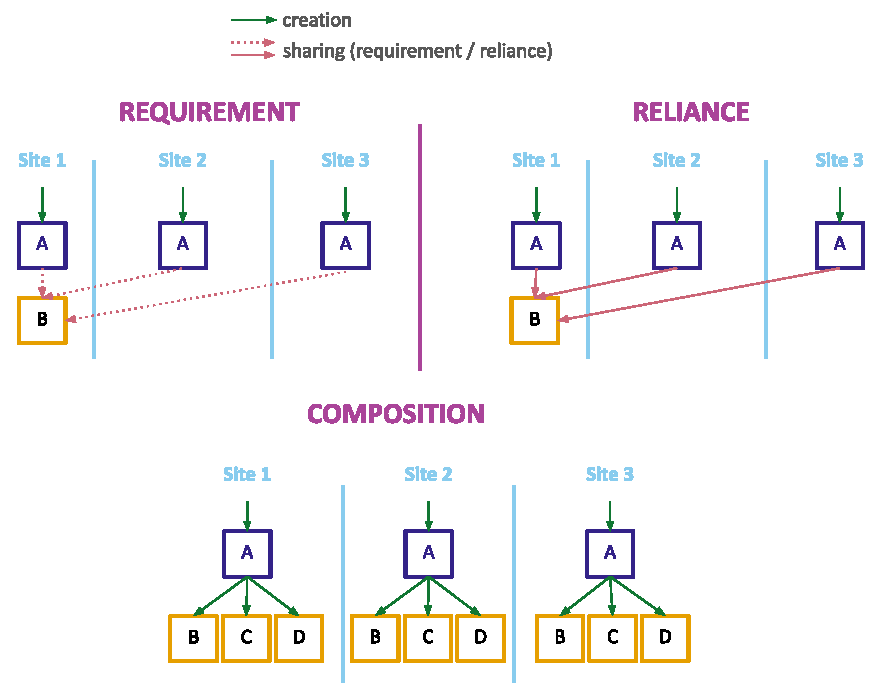
\includegraphics[width=0.76\linewidth]{figs/pdf/behaviors.pdf}
  \caption{Behaviors to observe following the dependencies}
  \label{fig:patterns}
\end{figure*}

As mentioned, the goal of the relationship model is to ensure that
Cheops operations are done thoroughly when the manipulated resource is
not elementary, but depends on other resources.
%
We discuss in this paragraph the various cases.

\begin{description}
\item[Requirement]%Under this relationship, in order to create a resource A, another resource is \emph{required}: resource B.
  For a replication scenario, the user have the choice to first
  replicate B everywhere A will be; in this case, the creation of A
  can be executed without specifying the location of B, it will be
  executed locally on each site.
  %
  The other choice is to specify the dependency in the creation
  request, which is represented in \autoref{fig:patterns}.
\begin{enumerate}
\item Using the sharing operator in the scope, the user specifies that
  a resource B required is on $Site 1$.
\item Cheops intercepts the request to get a resource from another
  site when it will be sent by the service needing it.
\item Cheops transfers the request to get resource B from $Site 1$.
\item Resource B is received and the usual flow is executed.
\item Since Resource B is only required for some operations, this
  dependency is stored in Cheops database for further usage (in these
  operations).
\end{enumerate}


\item[Reliance] This relationship follows a similar approach from
  requirement for replication.
  %
  The difference is with the involvement of Resource B through the
  life span of Resource A.
  %
  At any point if Resource B fails for both collaborations, resource A
  will result in a failure state.
  %
  The primary objective being to preserve the strong relationship
  between Resources A and B, Cheops needs to ensure the
  reachability of Resource B.

  As before, a user can still replicate Resource B to ensure that
  Resource A will not suffer from a network partition.
  %
  Otherwise, the process is the same as the requirement, except for:
  first, the dependency information needs to be stored in Cheops
  database for resource B to warn users against resources failures in
  replicas in case of a deletion of B.
  %
  Second, Cheops needs to warn the users of affected resources
  (replicas of resource A) in case of network partition that affects
  B, because they will be in a failure state.

\item[Composition] For replication scenario, a copy of resource A is
  created on the involved sites which in turn creates resources B, C
  and D on each of these sites with a \emph{cascading effect} from the
  normal, local execution of the creation of A.
  %
  An update on resource A for a secondary layer resource B, C or D is
  propagated across the involved sites and also follows normal
  execution on each site.
  %
  Network split brain is managed through the Raft protocol that
  ensures eventual consistency between all replicas.

\end{description}

Though this classification is still mainly theoritical, with some
implementations being currently studied, the implementation of the
rest of the approach will be presented in the next chapter.


\chapter{Cheops, our solution to push Cloud Applications to the Edge}
\label{chap:cheops}

In this chapter, I will present the implementation of the global
approach, and what we achieved to have our service mesh dedicated with
the purpose of pushing applications to the Edge by managing their
geo-distribution.
%
This service mesh is called Cheops.


\section{Towards a full implementation of our approach in Cheops}
\label{sec:cheops-v1}

In the appendix (\autoref{chap:first-approach}), I present the first
version of the implementation, that was a first step towards our
current approach.
%
In this section, we will discuss the current implementation, which is
still under development.

Cheops is a service mesh, with a proxy intercepting the request for
each service as the data plane.
%
The control plane is deployed on each site, as a service, as it is one
more service of the application instance.
%
In the rest of the manuscript, I will refer to ``Cheops'' as the
Cheops service deployed on each site; they all communicate between
each other to allow for collaboration, forming a service mesh with the
proxies.
%
Each of them maintains a catalog of the service instances on its site
to know how to contact them locally.
%
Each Cheops knows its neighbours and contact only the other Cheops
involved in a request, and they are responsible to contact the
involved services with their local catalog.
%
More importantly, to keep it generic, Cheops considers each type of
resources as black boxes.


In the next figures, we do not present the specific involved
endpoints, as the important part is the services involved.
%
Each service is shown as a rectangle, named as $Service X_i$ with
$Service X$ the name of the service and $i$ the identifier on the site
where it is located.
%
The proxies are represented as an oval around the services.
%
The Cheops databases are represented only when they are necessary.
%
Manipulated, involved resources are pictured as a small circle on
each service.

\subsection{Implementation of collaborations}
\label{subsec:collab-implem}


We will first detail how the three collaborations were implemented in
\emph{Cheops}, or at least some overview on how they should be
implemented.
%

\subsubsection{Sharing}

Sharing was a joint work envisioned by Ronan-Alexandre Cherrueau,
Adrien Lebre, Matthieu Simonin and Javier Rojas Balderrama with a
\acrshort{PoC} named OpenStackoïd~\cite{oid, CLRB19, CDLR+20}.
%
% Thus, sharing is not implemented in Cheops for now.

As explained in the previous chapter, \emph{sharing} is the
collaboration which allows a service instance to use a resource from a
service which is not the one assigned to its application instance.
%
This is the first way of leveraging the entire infrastructure, by
distributing different resources on different sites and allowing their
use from one site on another, enforcing the collaborative-then
principle.
%
It actually also enforces the local-first principle, because it allows
the execution locally, using only resources from other sites when
required.

\begin{figure}
  \centering
  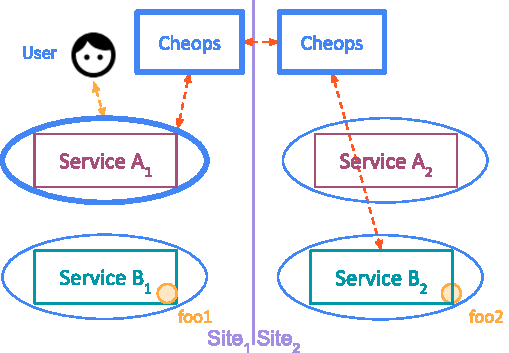
\includegraphics[width=0.7\textwidth]{figs/pdf/cheops-sharing}
  \caption{Sharing uses services instances from different sites}
  \label{fig:cheops-sharing}
\end{figure}

The typical example is getting a resource from a Service B on another
site for a Service A, the workflow presented as red arrows in
\autoref{fig:cheops-sharing}.
%
For example, if $Service A$ requires a $foo$ resource from
$Service B$, the command line given by users to request the use of
resource $foo2$ from $Service B_2$ on $Service A_1$ is:

\noindent {\small \texttt{application create a -{}-name bar -{}-sub-resource foo2 -{}-scope \{A: $Site_1$, B: $Site_2$\}}}
%

\begin{enumerate}
\item A user requests to create a resource $a$ on $Service A$ from $Site_1$
  (Service $A_1$), using a sub-resource $foo_2$ from $Service B$ on
  $Site_2$ (Service $B_2$).
\item The request is intercepted and transferred to Cheops (control
  plane).
\item Cheops extracts the scope from the request and interprets it, in
  this case, learning that it should be directed to the local
  $Service A$.
\item Cheops transfers the request to $Service A$, that executes it
  until it needs the sub-resource from $Service B$.
\item The outgoing request is intercepted, and at this point, is
  transferred to $Site_2$ for forwarding on $Service B_2$.
\item Cheops on $Site_2$ uses its catalog to find Service B endpoint
  locally and transfers the request to get $foo2$.
\item The service response (containing the resource itself) is finally
  transferred back to Service A through Cheops.
\end{enumerate}

Similarly to a local failure, if $Service B_2$ is not reachable, the
request cannot be performed.

We can see here that contrary to the intra-services collaboration we
talked about in~\autoref{sec:why-no} that requires dedicated code, our
approach use directly the response from another service instance,
which is offered by default.


\subsubsection{Replication}
\label{sssec:cheops-rep}

We will give here a first overview on how replication can be
implemented, a detailed version will be given later on, as it was the
specific collaboration I studied in our approach, and here, we give an
overview for all collaborations.
%
\emph{Replication} is the ability for users to create
and have available resources on different Edge sites to deal with
latency and split networks.
%
Replication main action is duplication: transfer the
request to every involved site and let the application execute the
request locally.
%

The operation does not simply consists though in forwarding the
request to the different instances.
%
Cheops keeps track of the different replicas in order to ensure that
future CRUD operations achieved on any replica will be applied on all
copies, maintaining eventually the consistency over time from the CRUD
point of view.
%
To do that, Cheops relies on a data scheme, called the replicant, that
links a meta-ID to the different replica IDs and their locations
(called the mapping in the previous chapter).
%
Replicants are located on every Cheops database on the sites involved
in the request to replicate, just as the replicas are located in every
application database on these same sites.


\begin{figure}
  \centering
  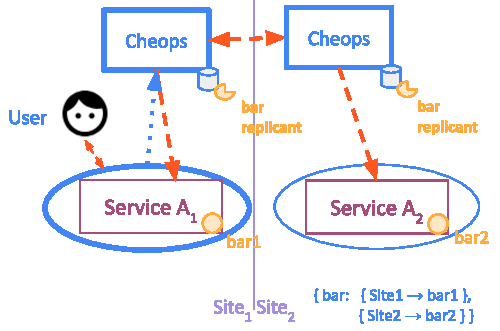
\includegraphics[width=0.8\textwidth]{figs/pdf/cheops-replication}
  \caption{Replication executes an operation on multiple instances}
  \label{fig:cheops-replication}
\end{figure}

\autoref{fig:cheops-replication} sums up the workflow to create a
replicated resource on two sites:

\noindent{\small\texttt{application create a -{}-name bar -{}-scope \{Service A:
    $Site_1$ \& $Site_2$\}}.}
\begin{enumerate}
\item A user sends a request on $Site_1$ to create two replicas of the
  \emph{bar} resource on $Service A$ from $Site_1$ and $Site_2$, \ie
  $Service A_1$ and $Service A_2$.
\item The request is intercepted and transferred to the local Cheops
  (control plane).
\item Cheops extracts the scope and interprets it, in this case, it
  needs to contact $Service A_1$ and $Cheops$ from $Site_2$.
\item Cheops creates the replicant, and passes the request to create
  it to Cheops on the other involved site ($Site_2$).
\item Both Cheops execute the request of creation of \emph{bar}
  locally, which is simply the request without the scope; the response
  is intercepted to fill the local IDs on the replicants and the
  response is transferred to the user, replacing the local ID by the
  meta-ID of the replicant.
\end{enumerate}

To provide eventual consistency, Cheops follows the Raft protocol,
with one replicant acting as the leader.
%
As for the other collaborations, it is crucial to understand that
since we manipulate the resources through the API their services
expose, we can only intervene from this point of view.
%



\subsubsection{Cross}

% This collaboration is the work from Geo Johns Antony and is still in
% progress.
% %
% It also has been preliminary and shortly studied by Karim Manaouil.
% %
% This work is given for a complete view of the approach, though the
% logic is not entirely defined, and thus subject to changes.

As mentioned earlier, Cross is not entirely mature, but has been
implemented in part in Cheops, and thus it is worth developing a bit
more.

\begin{figure}[hbtp]
  \centering
  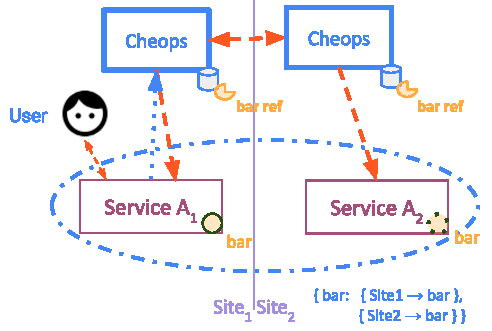
\includegraphics[width=0.8\textwidth]{figs/pdf/cheops-cross}
  \caption{Cross gives the illusion that multiple resources behave as
    a single one.}
  \label{fig:cheops-cross}
\end{figure}

%
An illustration of Cross is depicted in \autoref{fig:cheops-cross},
following this request:

\noindent{\small \texttt{application create a --name bar --scope \{Service A: $Site_1$ \% $Site_2$\}}.}

\begin{enumerate}
\item A user sends a request to create a resource specifying the
  involved sites in the Cross operation.
\item The request is intercepted and transferred to Cheops.
\item Cheops extracts the scope and interprets it.
\item Cheops creates the resource on the first site ($Site_1$) and
  passes the request to Cheops of other involved sites (here, $Site_2$
  only).
\item Cheops on $Site_2$ identifies the extended resource and creates
  an identifier within Cheops to forward to the deployed resource site.
\end{enumerate}




\subsection{Cheops architecture}
\label{ssec:cheops-archi}

% \todoref{cf  https://mqtt.org/}


The global architecture of our proof-of-concept is depicted in
~\autoref{fig:Cheops-architecture}.
%
Cheops follows a modular approach, composed of various microservices,
which are linked together through REST API protocol.
%
There is one Cheops per site and they monitor known Cheops
through heartbeats.

For redirection purposes, each Cheops has its own internal registry.
%
First, it stores information about its own site: the addresses of each
application service endpoint as a catalog or registry.
%
Second, it keeps the addresses of its Cheops neighbours to know where
to transfer the requests when needed.
%
%
Cheops never intercepts requests coming from a Cheops to an
application service to avoid looping.


\begin{figure}[hbtp]
  \centering
  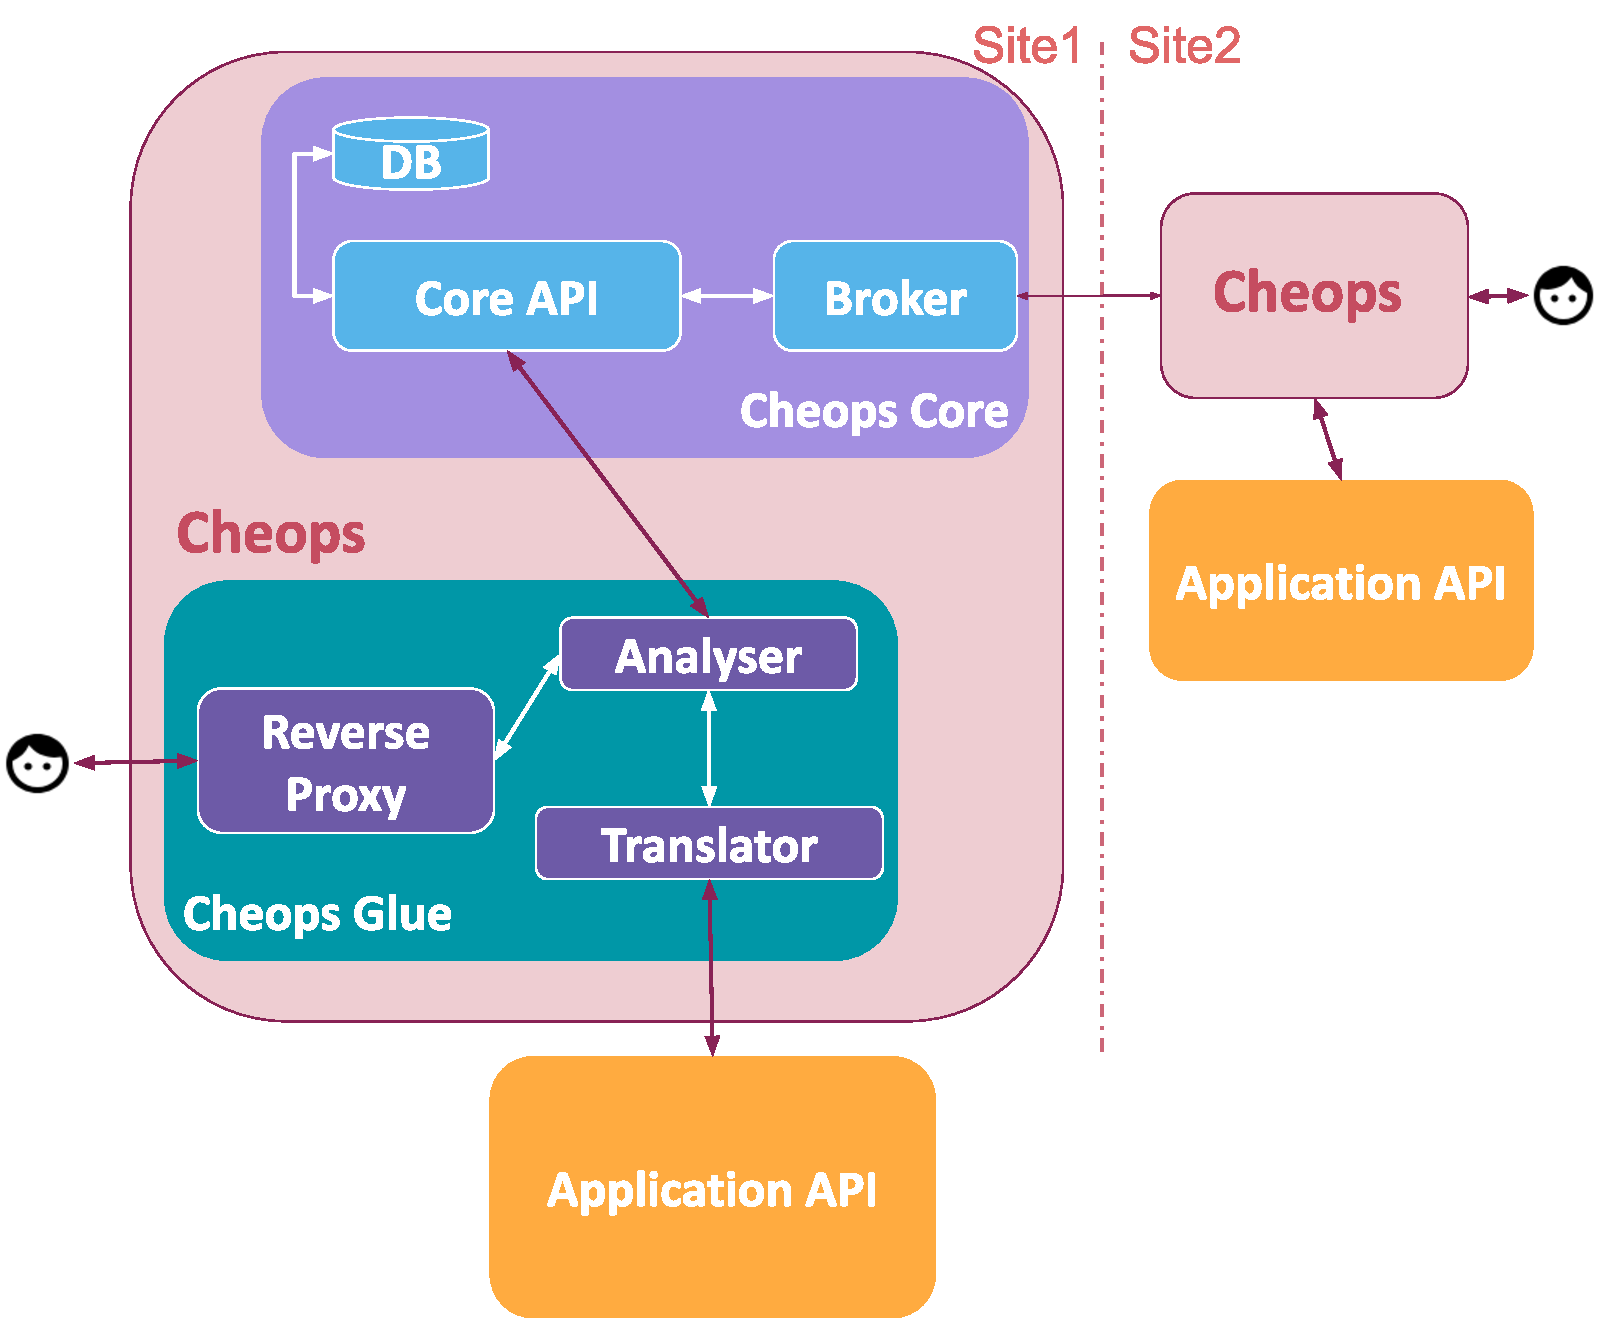
\includegraphics[width=.75\linewidth]{figs/pdf/cheops-architecture}
  \caption{Cheops architecture}
  \label{fig:Cheops-architecture}
\end{figure}
%

\subsubsection{Cheops internals}
%
The Cheops control plane is divided into two main components which are
Cheops Core API and Cheops Glue.
% The modular approach promises integration of various frameworks

\begin{description}
\item{\textbf{Cheops Core}} is the primary building block of Cheops.
  %
  It encapsulates the communication module, interface module (Core
  API) and the database.
  %
  The communication module provides the link between multiple Cheops
  instances, thus creating and maintaining a service mesh around the
  various involved clusters.
  %
  Since Cheops focuses on minimizing intrusive code changes of a
  deployed application, this module plays a significant role, while
  addressing the collaboration features of Cheops.
  %
  This module also communicates with the the Core API module in the
  Core.
  %
  The Core API is a management module created to interconnect all the
  services inside Cheops.

\item{\textbf{Cheops Glue}} is the second module of Cheops.
  %
  This module is designed to help Cheops Core translate Cheops API
  requests into the respective application API and vice-versa.
  %
  Core is designed to handle agnostic API requests which are
  irrespective to all the applications.
  %
  Cheops needs to convert these requests into application
  understandable API patterns.
  %
  Since each application has its own pattern for intercepting API,
  Glue is developed with respect to individual applications such as
  Openstack, Kubernetes, etc.
  %
  Thus, this module is not generic to every approach and has to be
  implemented to translate the requests, but still allows the
  externalization of geo-distribution concerns.
  %
  Glue acts as a first layer communication between users and Cheops by
  intercepting the data from the default CLI from the respective
  application using \scl.
  %
  The analyzer service in Glue evaluates the request and converts it
  into a generic request understandable by the Cheops Core API
  service.
  %
  On the other side, Cheops Glue provides a translator service which
  converts the requests received from the Cheops Core API service.
  %
  Cheops Glue will also manage the creation of extra business logic for
  divisibility property of cross collaboration
  (see~\autoref{fig:cheops-cross}) for specific types of resource.
  %
  The Glue also handles the network requirements and implements the
  relationship model (that we will only discuss in the future work
  part of the conclusion).
%Implementing a relationship model for resources dependent on the type of resource which requires a dedicated logic which will handle this.
\end{description}

The design of Cheops architecture is focused on a modular design
which makes it easier to manage and distribute.
%
It also provides the flexibility of enhancing each component or
individual service to scale it during peak usages.
%
It is available for any request specifying the usage of its hosting
site when it is not disconnected from the network (not offline) and
the users are also able to control this instance locally, making it
available at any time.
%
Cheops obviously offers the three collaborations proposed earlier.
%
It manages each collaboration without the need to modify anything in
the deployed application.
%
Finally, it maintains the consistency of the deployed applications
across the locations.




% \section{Scope-Lang interactions with Cheops}
% \label{sec:cheops-scl}



\section{A deeper dive into the replication}
\label{sec:cheops-replication}



As previously introduced, replication is the ability to create and
maintain identical resources on different sites: an operation on one
replica should be propagated to the others, dealing with faults and
disconnections and maintaining CRUD consistency based on our eventual
model.
%
Other consistency policies~\cite{ATB+16, ZW15} could be envisioned,
but let as future work as they do not change the general concept of
\scl/Cheops.
%
To get a better understanding of the point of replication, imagine a
user who needs a huge resource (like an ISO image) both at home and at
work.
%
The resource can be replicated at creation on both sites and it will
be the only time when the entire resource will go through the network.
%
This saves a lot of bandwidth, and is especially useful if there is a
partition between both sites, or if the user wants to work offline.


\subsection{Replication model}

A lot of this model has been discussed in~\autoref{ssec:scl-rep}
and~\autoref{sssec:cheops-rep}, so we will avoid as much as possible
repetitions, unless it can be explained differently for a better
understanding.

A replicant is basically a meta-identifier we generate along with a
list of mappings $site \rightarrow local\_identifier$ and a service
name (or identifier).
%
A replicant can thus be implemented for example as:

$ { meta\_identifier: [ site_n: local\_identifier_n, ...], service\_name} $

% We only store the location (site) of the replica and not the service
% used since it is possible to deduce the service with the incoming
% request.
% %
% This is subject to change depending of the evaluation of our
% prototype. We could store also the involved service and/or the type of
% resource involved.

It is important to know that for now, the service name has not been
used in the current implementation as the request given has been
enough to transfer to the correct service.

These replicants are stored in a database co-located to the Cheops
agents.
%
A copy of the replicant is stored on each site where its replicas are
located (the sites involved in the replication).
%
Cheops has an API of its own to allow the user to check the state of
operations, sites and inspect replicants.


\subsection{CRUD execution workflow}


First, to define what is the creation, update or delete workflow, we
have to define what they do in our consistency model and what are
their boundaries.

In replication, resources are only considered as black boxes seen only
as the API allows it, and thus the consistency maintained only by the
operations allowed by the API (usually CRUD operations).
%
Any modification made internally on one site by the application
without using the API cannot be expected to be replicated to the other
replicas.
%
Furthermore, any modification made on those replicas through the API
will be applied eventually to the other replicas.

%
The creation of resources replicated in an eventual consistency
implies that all replicas are identical at creation and will be
created eventually.
%
The update of resources created with the replication in an eventual
consistency implies that all replicas will be updated eventually,
whether the user specifies a scope or not in its request.
%
It is the same as updates for deletes.

About the boundaries, the operation obviously begins when the user makes
the request.
%
But for the end, we could consider that an operation ends either when
there is one response and is returned to the user, or when the
operation is executed on every site.
%
In an eventual consistency model, the latter (the operation done on
every site) can come a lot later than the first response.
%
%This is why we chose to decide for

%
It is important to know what happens in case of failure (partition,
disconnection, server failure) during the execution until the first
response, but also after, because the operation must be executed on
our replicas at some point.


In terms of the user view, the first response to arrive goes to the
user before it might be applied everywhere, so it is the
responsibility of the user to check with a request to Cheops or
directly to involved services and sites to know where the creation or
updates are already applied.
%
Users cannot assume because they received the answer the operation as
already been applied everywhere, some sites may have difficulty to
execute the request or may be even down.


\subsubsection{Creation}

The replication process to create a resource on $App_1$ and $App_2$
has already been detailed in~\autoref{ssec:scl-rep}
and~\autoref{sssec:cheops-rep}.
%
Therefore, we will not develop it further in this part, and the reader
can refer to these parts to know about it.




\subsubsection{Read}

%
Since the replicas are the same from the API level view, on a
probability of a replica not updated yet, read one replica or another
should not be different, so only one is needed to be returned.
%
Therefore, the process of reads is straightforward; to access a
specific resource, users must either request their site where one of
its replicas is (local-first) or specify in the scope on which
location a replica of the resource to read is (collaborative when
needed).




\subsubsection{Update}

After the creation of replicas, every request made to update (or
delete) is filtered to check if the id given corresponds either to a
replicant meta identifier or a local replica identifier.
%
Once again, this process is really long, so it is pretty costly, but
it ensures the consistency of the approach.
%
Ideally, it should be configurable, so the users can take
responsibility for the divergence of state in the replicas if they use
local replicas identifiers and everything is not analyzed.
% If it is, the request is transfered to every sites
% containing one of the replicas before being executed.
%
The process is quite similar to the creation, but does not generate a
new replicant or change an existing one.
%
It only applies an update to replicas and update the logs of
replicants.
\begin{enumerate}
\item
  A request for an update of a previously created replica is
  addressed to the endpoint of a service of one application instance.
%% \item
%%   Cheops uses its list of drivers to check which one to use, and sends
%%   the request to the correct one.
\item Cheops checks if the ID in the request exists in the replicant
  database.
  %
  If not, the request is sent back to the service to be executed.
  %
  If it is, the request is transferred to the Cheops agent storing
  the replicant leader.
  %
  It gets the corresponding replicant to find all replicas (and thus
  sites) involved.
  %
  The leader sends a vote to the replicants to have a consensus on the
  request.
  %
  When it gets the consensus, the operation is stored in its log.
\item The request is copied as many times as necessary (with the
  corresponding local identifier from the mapping so it will work
  properly on the different involved sites) and sent to the Cheops
  agent of involved sites.
\item
  Local Cheops agents send the request to the corresponding service on
  their site, which executes the request normally.
\item
  Each Cheops agent sends back the response to the Cheops agent where
  the replicant leader is.
\item This agent sends back the first response to the user, once
  again, with the meta-identifier where the local-identifier would be
  expected to notify the user that the replicas were updated.
\end{enumerate}



\subsubsection{Delete}

As for the update, a delete on replicas can be identified either by a
local identifier or the meta identifier.
%
The process is identical as the update's.

It is important in this subsection that adding replicas to a set of
pre-existing replicas situations have not been fully studied for
implementation yet, though they have been considered.
%
Conversely, the removal of a replicant from the set is important in
the processes of dealing with faults.


\subsection{Dealing with faults}


We define a fault as: a partition of network on an involved site
(disconnection), or a failure from this site, whether it is shut down,
out of order, or if the request cannot be executed for any reason (not
enough memory to create a resource for example).

It is also important to mention that if the site where the user sent
its request is faulty (does not work in any of the aforementioned
way), the request obviously cannot be executed.
%
The user can make the request to a more distant site, but this is one
of the advantage of replication.

Moreover, the ``during an operation'' can refer to two distinct
phases.
%
As we discussed before, the end of an operation can be seen
as: when a replica has been created/updated/deleted and the user has
been notified, and when the operation is applied to all replicas.
%
So ``during an operation'' is between the request of the user and
before one of these ends.
%
In our consistency model, this conveys no difference to the process.
%, but it does have an impact on the availability and state

If a site fails where a replica is supposed to be, other Cheops will
be informed due to its heartbeat (or rather lack of).
%
Any other operation received by the leader will then be retried
according to the log when the site comes back again.
%
Therefore, a site is considered to be eventually available again
unless it is removed.
%
If a site is removed from the system, every site that was hosting a
replica must delete the site from its mappings (from the replicant).
%
The leader will be in charge of this particular task, sending a
request to update the replicant.


\begin{description}

\item [Faults during operations]


The operation will be applied \emph{eventually} on all involved
sites.
%
This eventual consistency uses a consensus protocol, and in our
case, an implementation of Raft~\cite{OO14}.
%
For example, the leader's log allows to replay operations that are not
yet applied.
%
It is the responsibility of Cheops hosting the leader to ensure that
operations are applied eventually, by checking regularly operations
that have not been yet applied.


\item[Faults while there are replicas but not particular operation]

When a site fails while there are replicas somewhere without any
particular operation running, no heartbeat is received by other Cheops
agent and the replica is considered unavailable temporarily.

If a site where a replica is was partitioned at some point but could
be used locally, only read queries can be made, and these reads might
be stale (not be up-to-date to the operations that have been made on
other replicas). When rejoining the cluster, operations will be
applied on the site so it is up-to-date thanks to the leader's log.

\end{description}



\section{Testing Cheops replication}
\label{sec:validation}

We demonstrated the feasibility of our proposal on the Kubernetes
ecosystem.
%
The feasibility for the collaborations were studied for replication,
in which we manipulated replicated pods across two sites.
%
% Some experiments were made on the cross collaboration, too, but, since
% it is not the focus of this manuscript, we will not detail those here.


The experiments have been performed over two sites of the Grid'5000
experimental testbed~\cite{grid5000}, as it was used for the first
version of Cheops (see in the
appendix,~\autoref{chap:first-approach}).
%
The sites were completely independent of each other and located on two
sites of the infrastructure, namely Nantes and Rennes.
%
On each site, we deployed a Kubernetes cluster, each composed of one
master and one worker node, as well as Cheops.


%

\subsection{Current technology stack}


Cheops was deployed onto each site alongside an instance of the
application (Kubernetes), creating a \acrshort{P2P} service mesh
structure between these applications.
%
The primary goal was to create an initial development efforts as per
the architecture ~\autoref{fig:Cheops-architecture}.
%
These efforts provided the functionalities we proposed to create a P2P
service mesh, integrate collaboration mechanisms and flexibility to
extend to multiple applications.


For the initial study, Cheops was built on Golang, since it is very
adaptable to server-side scripting.
%
In order to create the service mesh, Cheops relies on a message broker
which provided P2P capabilities and a reliable messaging protocol.
%
Advanced messaging queuing protocol (AMQP) was chosen for our design of
the Cheops-to-Cheops communication (communication module of the Core).
%
RabbitMQ\footnote{\url{https://www.rabbitmq.com/} - Accessed
  2022-10-09} with P2P and AMQP messaging pattern were used for this
purpose.
%

For the database, the main requirement was to find a free and open
source database (for easier adoption) which could replicate the data
based on individual attributes.
%
After a survey, the conclusion made was that no particular database
existed which met all the required characteristics, and thus
ArangoDB\footnote{\url{https://www.arangodb.com/community-server/} -
  Accessed 2022-10-09} was chosen to be integrated into Cheops, to
allow us to have a NoSQL document store that could keep different
types of data.
%


The next component needed was the one that can intercept the users
requests in order to identify the request patterns and especially to
be able to get the scope in requests.
%
HAProxy\footnote{\url{https://www.haproxy.com/} - Accessed 2022-10-09}
was chosen to provide a lot of flexibility in order to integrate
between the application and Cheops.
%
\emph{Nonetheless, it is crucial to know that though we deploy HAProxy
in the current \acrshort{PoC}, we do not intercept requests and we
only use Cheops API to make the request.}
% \todomore{https://www.haproxy.com/blog/layer-4-and-layer-7-proxy-mode/}
% \todomore{we only use one proxy in lieu of one for each service}


In more details for the replication,~\autoref{fig:replicant} presents
the model for the Replicant structure, which is composed partly of a
slice (re-sizable array) of Replica objects.
%
In the Replica struct, there are information on the Site (name in our
case, but it could be an ID of a site for very large scale) on which
the Replica is, the ID of the local resource, and a Status that is not
used for now, but was added as a maybe simpler way to know if one
replica is reachable or not.
%
In the Replicant struct, we store the Meta-ID as expected, the
different Replicas (from the above struct), a Boolean to know if this
particular Replicant is the leader of the Replicants, and finally the
Logs of the different operations executed on the Replicas to maintain
consistency.
%
For those who are not used to Golang, the json information at the end
of the fields of the structures is for encoding and decoding to and
from JSON, so they can be passed with a REST request.




\begin{figure}
  \centering
  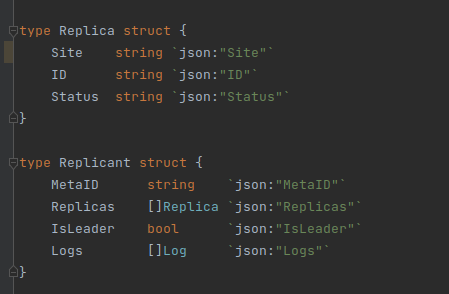
\includegraphics[width=0.8\textwidth]{figs/png/replicant-model}
  \caption{Actual replicant model in Cheops code.}
  \label{fig:replicant}
\end{figure}




\subsection{Experiments}
%We performed the feasibility study for the collaborations~\autoref{sec:collabs}. Replication and Cross were tested out on the Kubernetes framework in Grid'5000 testbed.

The artifact we used for the experiments is available on the Cheops
project page\footnote{\url{https://gitlab.inria.fr/discovery/cheops/}}
(around 3k lines of code).
%
It is a joint work from Geo Johns Antony and myself.


The goal of the experiments we performed was mainly to validate the
expected behavior and genericity on simple requests.
%
Further experiments are still needed, and as mentioned, some
experiments on cross have also been performed but will not be
presented here.


\autoref{table:replication} presents the commands tested and their
results.
%


\begin{table}[htbp]
  \centering
  \setlength{\tabcolsep}{10pt} % Default value: 6pt
  \renewcommand{\arraystretch}{1.3}
  \begin{tabular}{|l|c|l|}
    \cline{1-3}
    \multicolumn{1}{|c|}{Operation}                                                                        & \multicolumn{1}{c|}{Location} & \multicolumn{1}{c|}{Result} \\ \cline{1-3}
    \begin{tabular}[c]{@{}l@{}}\verb|kubectl create pod purple| \\ \verb|    --scope{Site1&Site2}|\end{tabular} & Site1   & Pod \emph{purple} created on Site1 and Site2  \\
    \cline{1-3}
    \begin{tabular}[c]{@{}l@{}}\verb|kubectl create pod violet| \\ \verb|    --scope{Site1&Site2}|\end{tabular} & Site2   & Pod \emph{violet} created on Site1 and Site2  \\
    \cline{1-3}
    \verb|kubectl get pod violet| & Site1  & Pod \emph{violet} from Site1 is displayed \\
    \cline{1-3}
    \verb|kubectl get pod violet| & Site2   & Pod \emph{violet} from Site2 is displayed  \\
    \cline{1-3}
  \end{tabular}
  \caption{Experimentations on Kubernetes - replication.}
  \label{table:replication}
  % \vspace{-15pt}
\end{table}

We created one pod \emph{purple} and one pod \emph{violet}
respectively on \verb|Site1| and \verb|Site2|, with the scope
specifying to create those pods as replicas on both sites.
%
This means we should have a \emph{purple} on \verb|Site1| and
\verb|Site2|, and the same for the pod \emph{violet}.
%
This corresponds to the commands
\verb|kubectl create pod purple --scope{Site1&Site2}| and
\verb|kubectl create pod violet --scope{Site1&Site2}|, respectively on
\verb|Site1| and \verb|Site2|.

Then we requested the pods \emph{violet} from each site to check if
they were present.
%
This corresponds to the commands \verb|kubectl get pod violet| on both
\verb|Site1| and \verb|Site2|.

%
Though this set of requests tests really basic functionalities, we
were able to ensure that the \emph{create} and \emph{get} operations
were working as intended.
%

Additional experiments are under progress to test \emph{update} and
\emph{delete}, as well as scenarios on the behavior of replicas in
case of network split to check the consistency.
%
A study on different types of resources to better check the genericity
is also required.
%
Especially, we used Kubernetes for this, because the approach has
already been tested on \os, but we did not try this particular
\acrshort{PoC}, so this could be a further important test.


\chapter*{Summary of the approach}
\label{chap:summary-cheops}


To fulfill the requirements stated in~\autoref{sec:principles}, using
different existing technologies and means, Cheops and \scl are a
solution to bring existing, service-based Cloud applications to the
Edge.
%
The main goal is allow any of these applications to be run on Edge
infrastructures without changed in their code, by taking into account
the properties of the Edge.


Cheops a service-mesh which main functionality is to manage the
geo-distribution of the Edge sites and the resources of the
applications.
%
Scope-lang allows users to define the execution location and
collaboration in their requests \textbf{dynamically},
\textbf{on-demand}.

With the application deployed on each site, the solution answer the
\textbf{local-first} requirement automatically.
%
The different collaborations, of which we presented three, namely
sharing, replication and cross, fulfill the
\textbf{collaborative-then} requirement.

By externalizing the geo-distribution concerns, the approach is
\textbf{non-intrusive}, and it is as \textbf{generic} as possible
by only considering resources as black boxes and using the application
API, with only the Cheops glue specific to the applications.

The Cheops service mesh functions in a \textbf{decentralized} and
\textbf{P2P} manner, and is designed with autonomous sites and some
collaborations, to be \textbf{resilient to network partitions}.


\clearemptydoublepage
\backmatter

\part*{Conclusion} % 16p
\addcontentsline{toc}{part}{Conclusion}
%\chaptermark{Conclusion}



% Purvis: God, I'm so tired.
% Johner: Sleep when you die, man.


\begin{comment}
* Discussion, future work and conclusion - 16p
** Discussion - 3p
** Future work for Cheops - 10p
*** Ownership Types - 4p
*** Classification - 4p
*** Other collaborations - 2p
** Conclusion - 3p
\end{comment}

\epigraph{\emph{Christie:} How many [..] are there?\\
\emph{Dr. Wren:} Twelve.}{\emph{Alien: Resurrection}}


\chapter{Discussion} % 3p
%\addcontentsline{toc}{chapter}{Discussion}
\label{chap:discussion}

This chapter is dedicated to discussions around the approach, its
inherent limitations and what could be done better or in the future.
%
There is an entire chapter (\autoref{chap:future-work}) for the
perspectives on the approach, but in this chapter, we will only talk
about small changes that could be done in the Cheops implementation
and would not fundamentally change the approach.

The first small point to discuss is the naming ``service mesh'' itself.
%
The approach is called service mesh because of the definition of
William Morgan~\autoref{chap:soa-SM} (page~\pageref{chap:soa-SM}).
%
It is a layer handling service-to-service communication that delivers
request through the topology of services of cloud native applications,
implemented as an array of proxy alongside the services, and the
application is not aware.
%
In Cheops, the only functionality is to help the application running
at the Edge by managing the geo-distribution of instances of this
application.
%
But Cheops also fulfills some of the functionalities of an API
gateway, if we consider this definition from IBM~\cite{api-gateway}:
%
\begin{quote}
  \emph{An application programming interface (API) gateway is software
    that takes an application user’s request, routes it to one or more
    backend services, gathers the appropriate data and delivers it to
    the user in a single, combined package. It also provides
    analytics, layers of threat protection and other security for the
    application.}

  \emph{An API gateway provides a single entry point for all API calls that
  come into an application, whether the app is hosted in an
  on-premises data center or on the cloud. It accepts requests that
  come in remotely and returns the requested data.}
\end{quote}
The functionalities of analytics, threat protection and security are
definitely not considered, but what is done is Cheops could be viewed
as a decentralized API gateway (with several entry points that are
only the same Cheops instantiated on every site).
%
Overall, the name ``service mesh'' has been chosen to help grasping
the idea of what we do more easily, but we have functionalities from
different ways to manage services from Cloud applications.


Our approach, as it as been said, takes into account different
interesting features or way to approach problems that have been presented
in the state-of-the-art, ~\autoref{p:soa}.
%
The closest approach is~\cite{MWY+17}, which uses some kind of sharing
collaboration for Glance, tracks ID of the resources, and has
autonomous instances of \os on each site.
%
Cheops differs mainly by being more generic and using different types
of collaboration to fulfill the single coherent view.


\section{Application version}

As discussed before in~\autoref{sec:principles}, the approach
relies on the modularity of service-based Cloud applications, so it is
not viable for any type of Cloud applications.
%
It requires microservices-based applications that exposes an API for
services communications.
%
These applications also need to be able to work on a single site since
they will deployed autonomously on every sites.
%
Moreover, it has been mentioned shortly, but every instance of the
services should have the same version so they have identical models of
their resources and they have the same API.

%
This can be restrictive as it is difficult for different actors on the
entire infrastructure to maintain the same version, as it has been
seen with \os, different businesses often have their own version of
the application and have different versions of the application, some
dating from several years; and it is actually the case sometimes in
the same actor with different
locations\footnote{\url{https://cleura.com/services/cloud-features/regions-and-services/}
  - Accessed 2022-10-12}.
%
This is mainly because it is difficult to update a running
application, but also because it is difficult for open-source
applications to be tailored for every use case possible.


\section{Consistency}

\subsection{Consistency from the API}

This approach ensures consistency at the service-level, but for the
resources they manage.
%
The only operations available to manipulate these resources are
therefore the ones exposed by the API.
%
Thus, the resources are maintained as identical as the API allows it,
but nothing more and any change on the resources that can be done
internally make the replicas diverge from others.
%
For example, in the \os case, VMs created through replication will
have the same specifications, but everything done internally on the
VMs will not be replicated to other VMs as the application API does
not allow to make these changes.

It is a limitation of the approach, but this consistency \emph{inside}
the resources is not desired as it requires to know the internals of
the application and reproduce it outside or add code inside the
application to provide an API.
%
% For example, nothing can be said about the consistency of two VMs
% booted through this process; their internal state will probably
% diverge, as expected.

\subsection{Better consistency}

Raft is a distributed consensus algorithm using an elected leader to
apply the changes made on replicas.
%
The leader sends changes to the followers and await confirmation of
the majority of followers to confirm the change before committing it.
%
In our case, since we cannot always assume it is possible to rollback
a change in a resource, we only ensure that a majority of nodes are
available before sending the request to be executed.
%
Thus, the consistency is only ensured eventually, when the changes
will be executed on all involved replicas.

% en fait ça sera ptêtre meme pas le cas mdr (si site revient pas)
As another consensus algorithm, Epaxos could be considered, to avoid
designated leaders~\cite{MAK13, TPO21}.
%
% Epaxos

The use of Conflict-free Replicated Data Types (CRDT)~\cite{PBS18,
  SPBZ11} is also currently under study for future versions of Cheops.


\section{What can be improved in Cheops}

First of all, it is important to mention once again
(see~\autoref{sec:validation}) that in our current implementation of
Cheops, in order to simplify the process, we decided to avoid the
interception part as it is mostly technical.
%
Nonetheless, it should be considered for the validity of
the approach as it could be a problem for some applications, such as
Kubernetes, as Cheops acts as a man in the middle attack.
%
Fixing these security concerns from Kubernetes is a problem for the
security, but also for the approach, because we would be meddling in
the business code.
%
On the other side, it is possible to monkey patch the Kubernetes API
as it as been done for \os in OpenStackoïd~\cite{CLRB19}.
%
In any case, we are still missing this part for Cheops, currently.


% deploiement de services (cf notebook)



% cluster peering de consul à check

From HYDRA's paper~\cite{JS20}, we could also implement the decision
of a new leader to be on the closest site in terms of latency to the
one that is currently unavailable.
%
This is debatable though, as the closest site from the previous
leader is not necessarily the closest to the user.
%
This brings the question of whether users should be able to decide
where the leader of replicants should be, in case of mobility, to
lower the latency for requests to the leader.
%
These are points to be considered for the future.

% \todomore{should i discuss the new cluster peering from consul, since
%   I talked about Consul in part3?}

% \todomore{should i talk about a complete solution that would manage
%   the lifecycle of the application also?}



\chapter{Towards a generalized control system: future work} % 12p
%\addcontentsline{toc}{chapter}{Future work for Cheops}
\label{chap:future-work}

\section{Mid-term deliveries for Cheops}

From what has been discussed in the previous chapter
(\autoref{chap:discussion}) comes a lot of work to consider for Cheops
to be thought and/or done sooner rather than later.

Moreover, there is still work to consider from the theoritical views
we have on Cheops, such as more collaborations
(\autoref{ssec:more-collabs}) and the classification of resources
(\autoref{sec:classification}).
%
The classification in particular is under heavy discussions currently,
and an answer on how to use it with a dependency tree has been studied
thoroughly in the PhD work of Geo Johns Antony.


\section{Ownership Types to prevent meaningless collaborations: the long haul} % 4p
%\addcontentsline{toc}{section}{Ownership Types}


This perspective has been the main focus of my thesis for some time
and was not explored further after it has been set on the side to
focus on the global approach and replication.
%
Most of this section comes from our research report~\cite{CDLR+20} and
has not been peer reviewed.
%
This work comes in part from of the observation we made from the
exploration of using geo-distributed databases to push Cloud
applications to the Edge~\cite{DCL18} that sharing some resources make
no sense.


As said many times before, the scope, in our proposition, is built by
users according to their needs.
%
But this human defined scope is error prone, first of all because of
potential typing errors, but moreover, users might not be well
informed of the availability of a resource.
%
The problem arises when sharing resources is that some sharing are
fallacious because \emph{resources exist in a specific scope}.
%

To better illustrate this, we use an example scenario from \os: ``Boot
of a VM attached to a flat network''.
%
In \os, a flat network is often used to attach a VM to an existing
physical network, and the command would look like (omitting some
specifications from other services):
\begin{lstlisting}[numbers=none]
openstack server create my-vm --network flat
\end{lstlisting}

%
Figure~\ref{fig:network-solo} depicts how a request is made on only
\sOne with the ``192.168.0.0/16'' physical network.
%
After the user issued a boot request (\textcolor{CbBlue}{step 1}), the compute service
requests for a port on the flat network (\textcolor{CbBlue}{step 2}).
%
A port is a specific resource containing the information to attach the
VM to the network.
%
It includes a mac and IP address, henceforth the user can reach the VM
according to them at the end of the boot (\textcolor{CbBlue}{step 3}).
%
In a local setup, everything works as expected: the VM is reachable at
``192.168.0.3'', because this network has been set up on this site.

\begin{figure}[htbp]
  \centering
  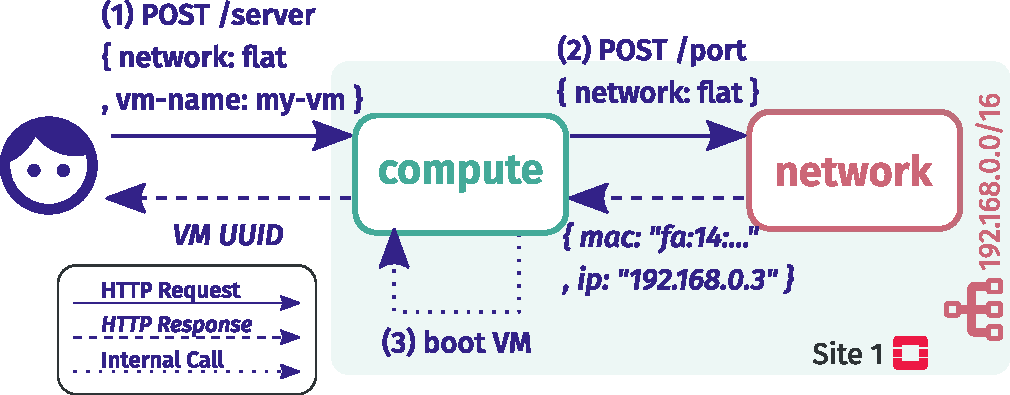
\includegraphics[width=.75\linewidth]{./figs/pdf/network-solo.pdf}
  \caption{Boot of a VM attached to a flat network locally }
  \label{fig:network-solo}
\end{figure}

Now, if we consider two different sites, with \sTwo also having a
physical flat network, but on a different domain (\ie ``10.0.0.0/8'').
%
Therefore a problem may occur if the user wants to use the share
operation such as ``boot a VM on \sOne using the flat network from
\sTwo''.
%
This operation can be expressed in \scl with the following command:
\begin{lstlisting}[numbers=none]
  openstack server create my-vm --network flat \
  --scope { compute: Site1, network: Site2 }
\end{lstlisting}

\begin{figure}[htbp]
  \centering
  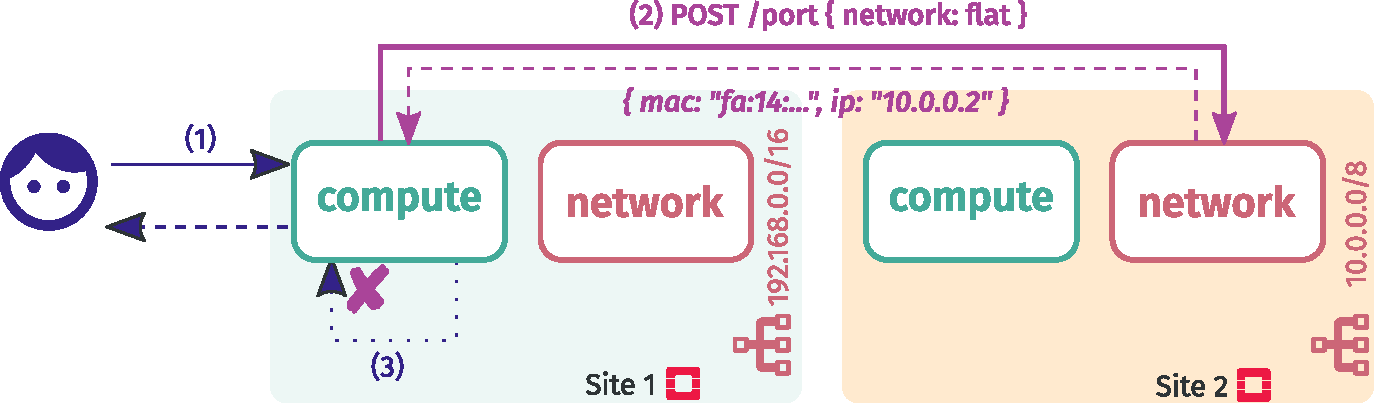
\includegraphics[width=.9\linewidth]{./figs/pdf/network.pdf}
  \caption{Launching a VM with a network, using collaboration}
  \label{fig:network}
\end{figure}

Such an operation makes no sense, as it is presented
in~\autoref{fig:network}.
%
\sTwo returns a port for its physical network (step 2 response) as it
usually would.
%
It includes the IP address ``10.0.0.2'' that is going to be used by
the VM in \sOne (step 3).
%
Unfortunately, \sOne has a different physical network
(``192.168.0.0/16'').
%
Therefore, though this operation is executed successfully, the VM
created with this address becomes unreachable.


Similarly to name bindings in programming languages, we say that
resources have a scope that defines their \emph{visibility}.
%
This scope could be local to one application instance (\eg in our
example, a physical network should only visible by its local site).
%
Or it could be global to all application instances (\eg in OpenStack,
an image is visible by all instances).


Sharing a resource with a local scope such as in
Figure~\ref{fig:network} is a problem.
%
Here, the VM is created with \emph{side effects} that are associated
with this creation.
%
These effects are costly because they uses multiple resources while
being of no use (since the VM will be unreachable).
%
More importantly, it is impossible to define a general rollback
strategy that undo all these side effects.
%
So it is crucial that each resource sharing is validated before its
execution.

A naive approach to identify invalid resource sharing would be to
exhaustively list all correct ones.
%
While it is a pragmatic approach for a specific use case, it does not
offer extensibility and lacks of generality.
%
This approach could work for one given version of an application, but
any changes or additional features would result in invalidating the
aforementioned list.

To avoid such dependencies to one specific application, we propose to
leverage memory access control techniques.
%
In programming, a particular information has a validity in its own
memory context.
%
This information can be used in different contexts as long as there is
a \emph{reference} that enables its access.
%
Sharing and copying this reference into other pointers leads to a
well-known issue called pointers aliasing (\eg dangling pointers).
%
An simple example of a dangling pointer is presented
in~\autoref{fig:dangling-pointer}.
%
A pointer ptr1 references an object by its address in the memory.
%
At some point, a copy of the pointer (ptr2) is made, for example for a
shallow copy of the object.
%
The object goes out of scope, either because it was a local variable
and the function is done, or because a user deletes it.
%
The memory is de-allocated, but ptr2 still points to it.
\begin{figure}[htbp]
  \centering
  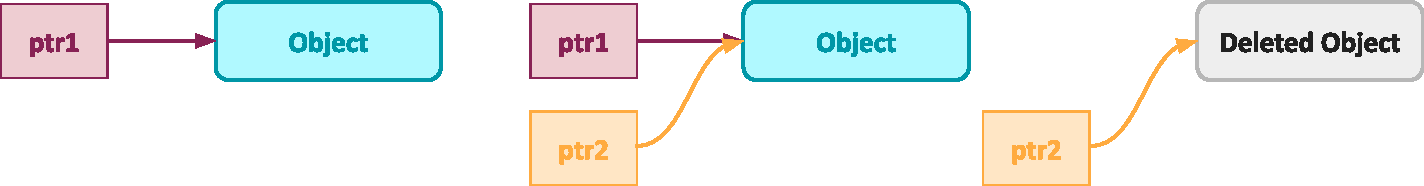
\includegraphics[width=.9\linewidth]{./figs/pdf/dangling-pointers.pdf}
  \caption{Dangling pointer example.}
  \label{fig:dangling-pointer}
\end{figure}

%
Among the solutions that have been proposed to deal with this issue,
the ownership types (\acrshort{OT})~\cite{CPN98,BLS03} has defined the
notion of containment.
%
At coarse-grained the idea is to only allow the owner of the memory
space to access it, preventing references sharing and copying.

We propose to use in the future this concept in \scl to prevent wrong
collaborations.
%
In the network scenario, \sTwo owns a network resource but the user
shares its reference with \sOne.
%
It resembles the dangling pointer problem: the scope of the network
is \sTwo and so cannot be reached by \sOne.
%
The sharing of this resource must be prevented.

Using \acrshort{OT}, it becomes possible to specify the scope of this
resource (\ie a type that defines which \os instances is its owner).
%
This type can be used in a type-checker to prevent any wrong sharing a
priori.
%
The pseudo-code in Figure~\ref{lst:OT} shows the OT annotations
and type-checking of our network scenario.
%
We first define the services (l.~1-4). Then instantiate them with
Compute in \sOne and Network in \sTwo (l.~6-9).
%
Finally, we create a VM on \sOne using a reference to the network from
\sTwo (l.~11-12).
%
Here, the type-checker complains about the ownership of the network.

\begin{figure}[tb]
  \lstset{moredelim=[is][\color{Purple}]{$$}}
  \begin{lstlisting}
class Network$<m>$:  # Network service
  def getFlatNetwork() -> $m/$FlatNetwork: #...
class Compute$<m>$:  # Compute service
  def createVM(network: $m/$FlatNetwork)-> $m/$VM: #...

# Code of the OpenStack CLI for
# > openstack server create --network flat
network: $Site2/$Network = Network$<Site2>$()
compute: $Site1/$Compute = Compute$<Site1>$()

flat_net: $Site2/$FlatNetwork = network.getFlatNetwork()
compute.createVM(flat_net)
#                ^ mismatched types:
#                  `createVM` expects `Site1/FlatNetwork`,
#                  but found `Site2/FlatNetwork`.
  \end{lstlisting}
  \caption{Ownership types {\color{Purple}(in purple)} to prevent invalid collaborations}
  \label{lst:OT}
\end{figure}

The \acrshort{OT} proposal should not need changes in the business
code of the application.
%
However, it requires to type services API in addition to implement a
type-checker.

This ownership types approach should be developed further to help
ensure that sharing of resources will be done in a manner that
prevents non valid sharing.

This approach is a long haul to consider and implement and thus is
considered for the distant future of Cheops.



\chapter{Conclusion} % 3p
%\addcontentsline{toc}{chapter}{Conclusion}


The Edge computing paradigm has shifted the way applications need to
be designed to cope with a hostile environment where disconnections
are the norm rather than the exception.
%
With the need for low latency and robustness against disconnections,
it is difficult to envision using existing applications designed for
the Cloud at the Edge.

To run such an application on such a widely spread infrastructure, it
is crucial to consider scalability as well as locality and tolerance
to faults in the infrastructure.

In this thesis, I have studied how it is possible to avoid creating
new applications specifically for the Edge, but rather use existing,
service-based Cloud applications.


\section*{Summary of the approach}

To deal with the latency and disconnections, the application used need
to be deployed entirely on each Edge location, which allows for a
local-first approach, where the application work autonomously on each
location.
%
Then, to allow for a single coherent system cherished in distributed
systems, for mobility and the usage of the entire infrastructure, it
is mandatory to give the application the ability to be
collaborative-then.
%
To allow for site collaborations, we need to be able to manipulate the
location of request executions.

As Cloud applications can be huge, the solution needs to be generic
and non-intrusive to avoid treating location information in the
business code, so it is necessary to externalize the geo-distribution
concerns outside of the application.
%
Finally, because the Edge infrastructure is highly dynamic (with sites
disconnections and failures) and to allow users to decide the location
of the request execution (\eg for privacy), it is important to give
them the ability to choose it on-demand, dynamically.

The study of the state-of-the-art gave good hints on how to make all
of these requirements happen in a P2P, fully decentralized manner,
though it did not provide an entire solution for all of them.

%
A service-mesh dedicated to the management of the geo-distribution and
collaborations between applications was the solution that fit all the
requirements to put existing Cloud applications at the Edge.
%
To allow this approach, \scl is the DSL that supports the
user-defined, on-demand, fine-grained request descriptions.
%
The modularity of the service-based Cloud applications and the way
their services communicate with each other through REST APIs are the
major elements that helped our approach, by allowing the forwarding of
requests, on top of which different collaborations are possible.


The current version grants three types of collaborations: sharing,
that uses a resource from another site, replication, which allows
users to put identical resources on different sites, and ensures that
they will stay identical from the API point of view, and cross, which
allows resources spanning across different sites.
%
These three collaborations enable the use of resources locally first,
and across sites when needed.
%
They help to lower latency, allows redundancy, fault tolerance, and
along with the users defined requests, they give the users the ability
to choose at fine-grain where their requests will be executed and
which resources to use, which also ensure their privacy, as they can
select what sites they trust.
%
In particular, the replication uses well known algorithms and logic to
ensure consistency and tolerance to fault partition and it allows
users to manipulate whichever replicas is closer/available.

As perspectives to improve this work, I gave hints of possible
extension of collaborations thanks to the genericity of the approach
regarding resources.
%
I also presented the classification of dependencies to ensure the
proper manipulation of linked resources.
%
Finally, for the long haul, I explained how to prevent non-valid
sharings through the use of ownership types.
%

\section*{Overview of the parts and chapters}

This manuscript was built as this following description:
\begin{description}
\item[The introduction] asserts the problematic of this manuscript. To
  be more descriptive, the goal is mainly to answer the question: is
  it possible to bring Cloud applications to the Edge? And with even
  more specifics, can it be applied to Cloud infrastructures
  management applications, and could we use a service-mesh approach to
  do it?
\item [\autoref{p:context}] explains the context of the manuscript.
  \begin{description}
  \item [\autoref{chap:cloud}] described the Cloud overall to give the
    reader a context of what the Cloud is. It gave a view of how Cloud
    applications function and how to manage the Cloud infrastructures to
    give a basis to understand the approach presented in this thesis.
  \item[\autoref{chap:edge}] presented the Edge and its challenges to
    explain on which expectations we were going to build our
    approach. We then defined the principles which we think are
    necessary to follow when developing or adapting an application in
    the context of the Edge.
  \item[\autoref{chap:cloud-app-to-edge}] described in more details
    how it is possible to adapt a Cloud application for the Edge and
    why the required collaborations are not good solutions for me as
    they imply really intrusive changes.
  \end{description}
\item [\autoref{p:soa}] depicts the State-of-the-art regarding the
  management of applications at the Edge, whether they were natively
  built for it or brought from the Cloud.
  \begin{description}
  \item[\autoref{chap:comparison} \textnormal{and}
    \autoref{chap:soa-conclusion}] serve as introduction and conclusion
    for the State of the Art. The first present how we evaluated the
    literature and the latter present the overall comparison.
  \item[\autoref{chap:soa-edge-infra}] presented six approaches to
    manage the infrastructure and more importantly, applications on top
    of it. It also presented in \autoref{chap:soa-SM} to of the most
    known service meshes to better understand how they function and how
    they behave regarding our requirements.
  \item[\autoref{chap:soa-dev-edge-app}] showed two different approaches
    to develop an Edge-native application or adapt an existing one with
    intrusive changes.
  \end{description}
\item [\autoref{part:cheops}] introduces my approach to bring Cloud
  applications to the Edge using a service mesh like aproach.
  \begin{description}
\item[\autoref{chap:overview}] explained our own theoretical approach
  to respond to the expectation we presented in
  \autoref{sec:principles}.
\item[\autoref{chap:cheops}] presented in more detail the PoC we
  develop to correspond to the aforementioned approach, in particular
  the way the replication is implemented and how it was tested.
\end{description}
\item[The conclusion chapters] above presented discussions about our
  approach, its limitations and different perspectives to improve it.
\end{description}


% \todototoc
% \listoftodos[TODOOOOs]

%\pagenumbering{roman}
\clearemptydoublepage
\part*{Appendix}
\addcontentsline{toc}{chapter}{Appendix}
\label{p:appendix}


\chapter*{From Consul to Cheops: first tests on a dummy Cloud Application}
\label{chap:first-approach}

% Golic: In an insane world, a sane man must appear insane.

% \subsection{First version of Cheops: a static approach}

During 2021 spring, I supervised two interns, Matthieu Juzdzewski and Arnaud
Szymanek, worked on a first adaptation of our approach with the goal
of giving information on using a service mesh to implement the
theoritical approach given in~\autoref{chap:overview}.

In this first version, the idea was to have an entire instance of an
application on each site we want, and create a Cheops agent that would
also stand on each site.
%
These agents would be responsible to interpret the requests and
transfer them according to the \scl.
%
Also on each site, a reverse proxy besides every service, transferring
their requests to the local Cheops agent for interpretation.
%
% Agents communicate between each other and check each other status via
% heartbeats.
%
This implementation used Consul service
mesh\footnote{\url{https://www.consul.io/}} and
Envoy\footnote{\url{https://www.envoyproxy.io/}} as reverse proxy to
intercept and redirect, when needed, the requests.
%
% It is also worth noting that Envoy intercepts inbound and outgoing
% requests from services except for requests coming from Cheops agents.

The starting point for this work was we needed three components:
\begin{itemize}
\item intercepting/forwarding requests
\item knowledge of the services of the target application and their
  endpoints
\item extraction and interpretation of the scope in the requests
\end{itemize}

As it happens, a service mesh can execute the two first requirements,
the last needing to be implemented ourselves because it is \scl
specific.
%
As we discussed in~\autoref{chap:soa-SM}, Envoy works as a sidecar
proxy for every service and allowed for interception of requests.
%
Consul also uses a catalog that can be used dynamically to register
and unregister
services\footnote{\url{https://developer.hashicorp.com/consul/docs/discovery/services}
  - Accessed 2022-09-25}.

In this first version, there were two different components for Cheops:
the \emph{core} and the \emph{connector}.
%
The core received all requests to extract the scope, interpret where
to send the request and forward it.
%
If an address was local to the application instance (on the same
site), it used the Consul catalog to get the corresponding service
endpoint; otherwise, it was sent to the connector.
%
The connector was responsible to send a request on a distant host by
using a dictionary of known sites, and then the distant connector to
the corresponding service on its own site.

Unfortunately, with the complexity of the service mesh and proxy, this
work was working only on a simple use-case using two services
(ServiceA and ServiceB), which only purpose was for the first to call
for a resource on the second, to test if the sharing collaboration can
be achieved.
%
The original goal was to use Google Cloud Platform Online Boutique
Demo\footnote{\url{https://github.com/GoogleCloudPlatform/microservices-demo}},
but the purpose of this particular demo is to show the Anthos service
mesh usage, and thus was not really designed to manipulate the
resources inside.
%
This is why we deferred to two simple services with basic
functionalities and calls.
%
Moreover, in this version of Cheops, Envoy was configured to only
intercept and redirect requests for each service through a
ServiceRouter configuration.
%
Each service thus required a specific configuration to do so, and a
specific endpoint in Cheops.

\begin{figure}[htbp]
  \centering
  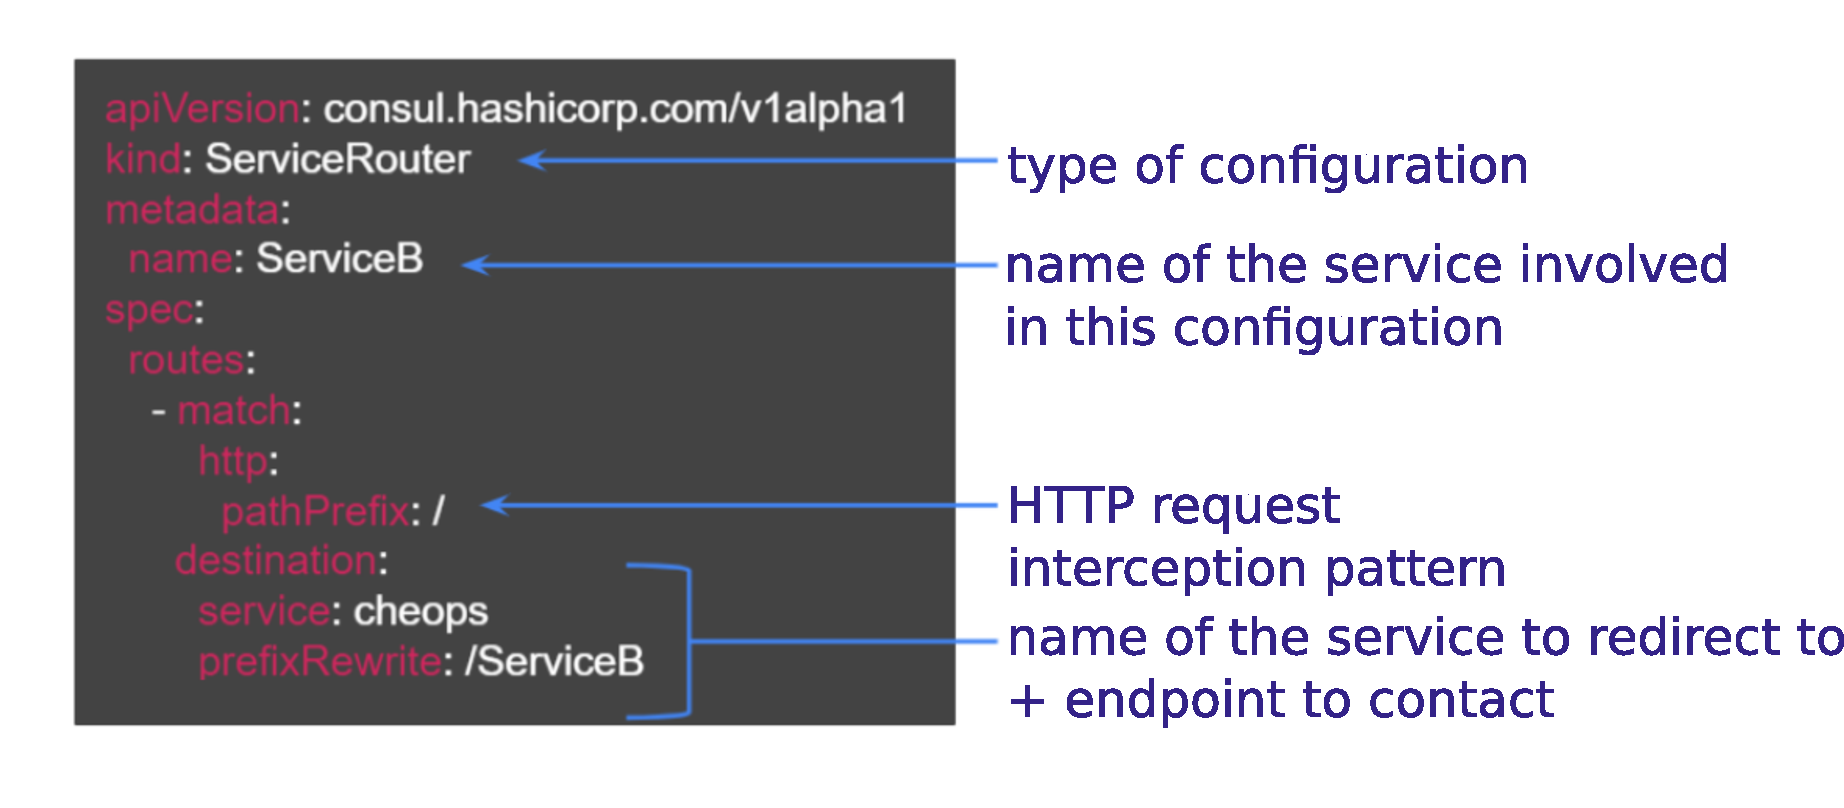
\includegraphics[width=\textwidth]{figs/pdf/cheopsv1-config}
  \caption{Configuration of a service in Envoy in the first version of Cheops.}
  \label{fig:cheops-v1-config}
\end{figure}

\autoref{fig:cheops-v1-config} shows the type of configuration that
was done to achieve the redirection to Cheops core.
%
For each ServiceB (metadata $\rightarrow$ name), every request will be
intercepted (the prefix is $/$), and will be redirected to the Cheops
service, at the endpoint \verb|/ServiceB|.
%
Thus, Envoy will redirect indiscriminately every request that comes
to ServiceB to Cheops for checking.


\begin{figure}[htbp]
  \centering
  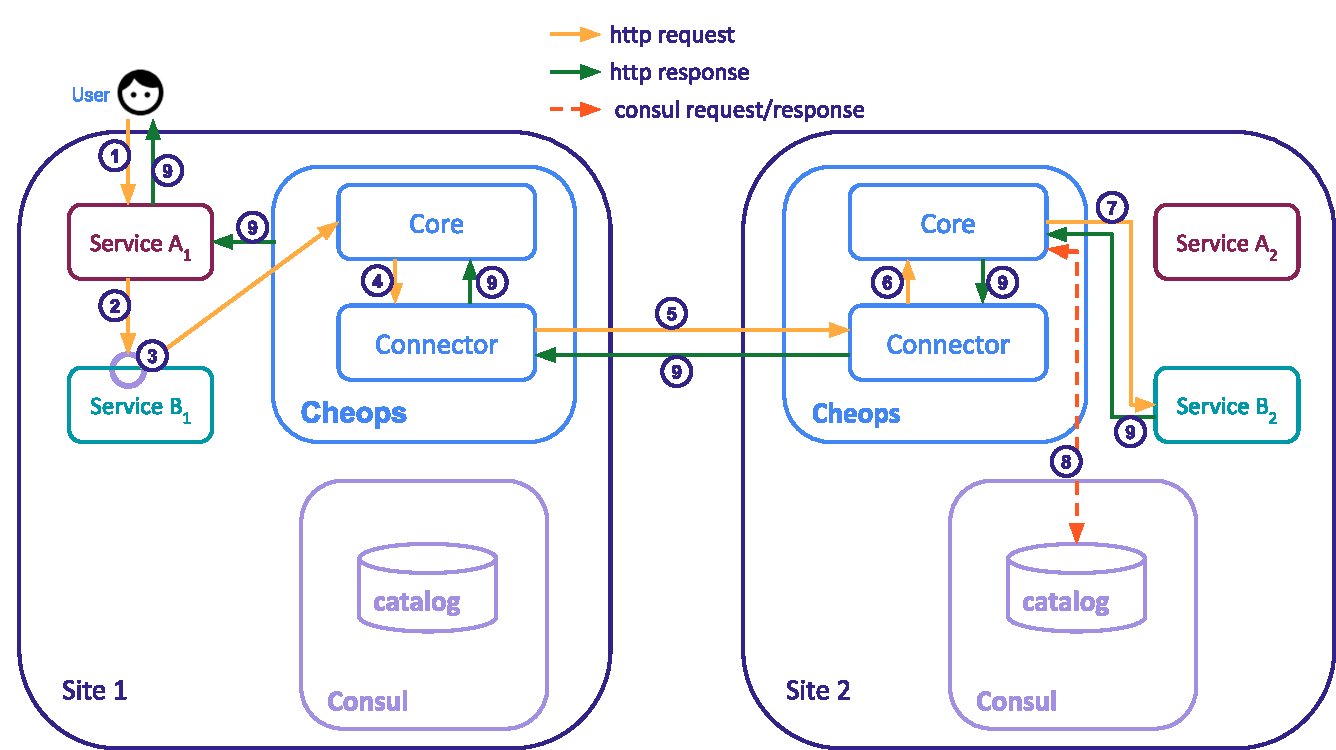
\includegraphics[width=\textwidth]{figs/pdf/cheopsv1}
  \caption{Workflow of a sharing request in the first version of Cheops.}
  \label{fig:cheops-v1}
\end{figure}

\autoref{fig:cheops-v1} presents the workflow of a request to use
$ServiceA_1$ and $ServiceB_2$, which means to use ServiceA on Site 1
and ServiceB on Site 2.
%
ServiceA has an endpoint $e$, which is called with an HTTP request:
\verb|http://address/ServiceA/e|.
%
ServiceB has an endpoint $h$, which is also called with an HTTP request:
\verb|http://address/ServiceB/h|.
%
This particular endpoint $h$ is the one called by ServiceA to execute
the workflow called with the endpoint $e$.
\begin{enumerate}
\item The request is made to use endpoint $e$ of ServiceA such as \\
  \verb|curl http://address/ServiceA/e -H "scope: ServiceB/Site2"|,
  with the scope thus integrated in the header.
\item To complete the workflow, ServiceA contacts the $h$ endpoint of
  ServiceB.
\item The prefix ``/h'' is recognized as an interception pattern for
  Envoy; the request is effectively intercepted and redirected to
  Cheops core on its /ServiceB endpoint.
\item The core extracts, interprets the scope and sends the request
  toward the connector since it cannot serve the request locally.
\item The connector finds in its registry the IP address for Site 2
  and transfers the request to Cheops connector on Site 2.
\item The connector on Site 2 redirects the request to its local core.
\item The core asks Consul catalog to get the address of the local
  ServiceB required; then finally transfers the request to this
  $ServiceB_2$.
\item The response from ServiceB is transferred back to $ServiceA_1$
  where the resource will be used to complete the workflow.
\end{enumerate}

This work on the first version of Cheops has been validated on two
different sites (Nantes and Rennes as Site 1 and Site 2) on the
Grid'5000 testbed~\cite{grid5000} (see~\autoref{fig:grid5000}).
%
The services have been deployed as Docker Containers through
Kubernetes.


\begin{figure}
  \centering
  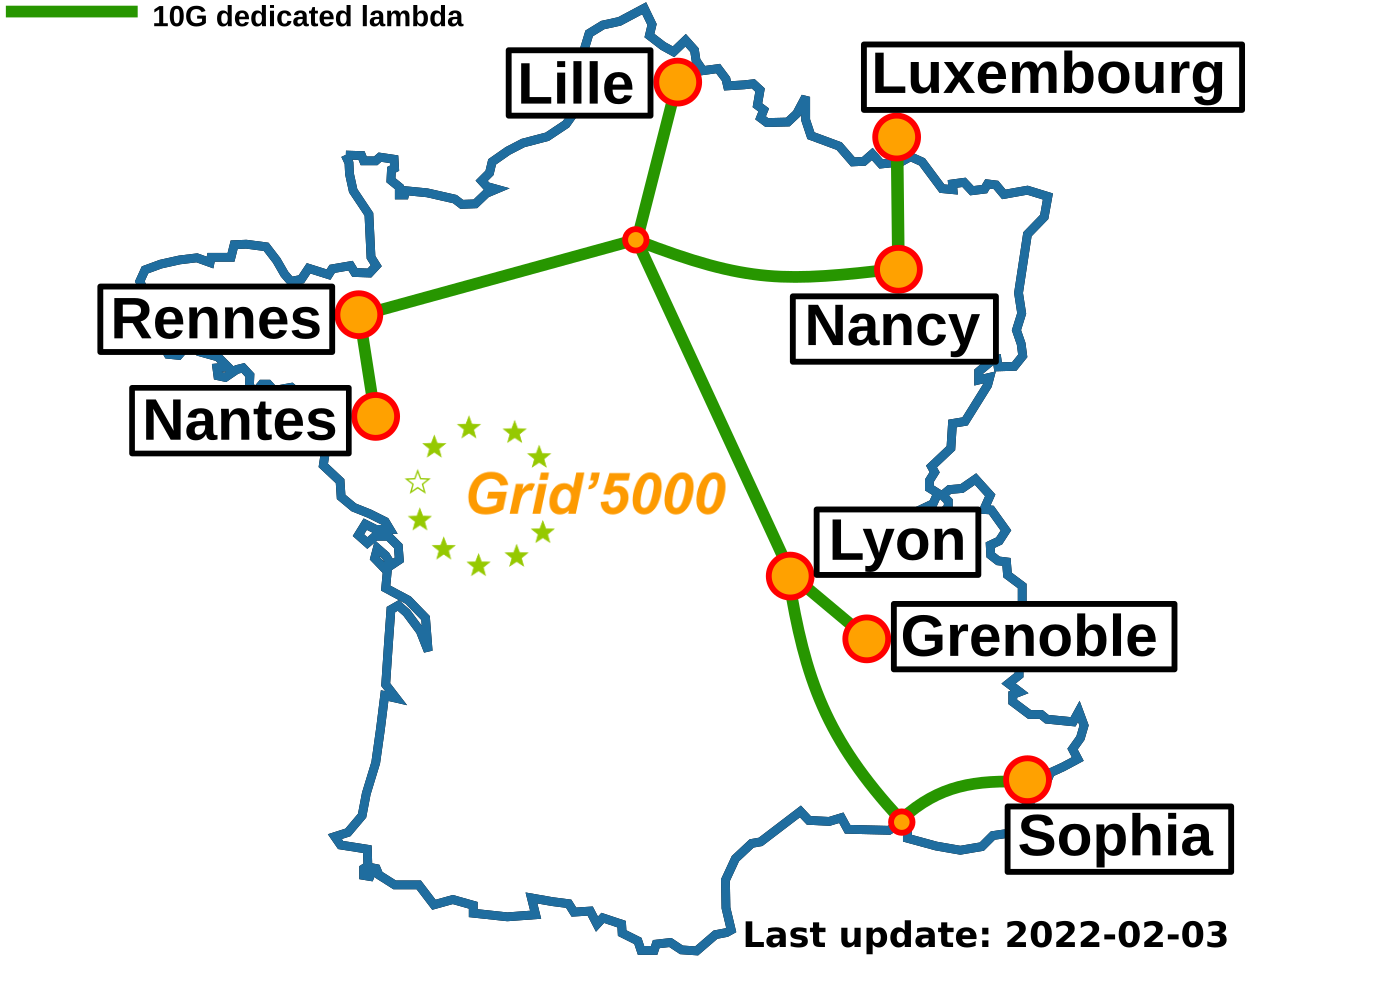
\includegraphics[width=.6\linewidth]{figs/png/Renater5-g5k.png}
  \caption{Grid'5000 and the Renater network.}
  \label{fig:grid5000}
\end{figure}

The experiment only showed it is possible to use a resource from
another site with sharing: ServiceA prints a string coming from
ServiceB.
%
The value of the string was ``I'm from Site 1'' on $ServiceB_1$ and
``I'm from Site 2'' on $ServiceB_2$.
%
The request sent to $ServiceA_1$ was:
\verb|curl http://localhost:1234/ServiceA/e -H "scope: ServiceB/Site2"|
and ServiceA printed ``I'm from Site 2''.

As mentioned, this version required an endpoint for every service
hard-coded in the Cheops core.
%
Moreover, Consul and Envoy had much more functionalities we did not
required, so we decided to do our own light service mesh.


This version of Cheops is available on the Cheops project
page\footnote{\url{https://gitlab.inria.fr/discovery/cheops/-/tree/v0.1.0}}.


\clearemptydoublepage
\chapter*{Publications}
\addcontentsline{toc}{chapter}{Publications}
\label{chap:publications}


\section*{\cloud~~Conferences}

\begin{description}
\item[ICSOC 2022] Delavergne, M., Antony, G.J., Lebre, A. (2022). Cheops, a Service to Blow Away Cloud Applications to the Edge. In: Troya, J., Medjahed, B., Piattini, M., Yao, L., Fernández, P., Ruiz-Cortés, A. (eds) Service-Oriented Computing. ICSOC 2022. Lecture Notes in Computer Science, vol 13740. Springer, Cham., doi: \href{https://doi.org/10.1007/978-3-031-20984-0_37}{10.1007/978-3-031-20984-0\_37}.
\item[Euro-Par 2021] Cherrueau, RA., Delavergne, M., Lebre, A. (2021). Geo-distribute Cloud Applications at the Edge. In: Sousa, L., Roma, N., Tomás, P. (eds) Euro-Par 2021: Parallel Processing. Euro-Par 2021. Lecture Notes in Computer Science(), vol 12820. Springer, Cham., doi: \href{https://doi.org/10.1007/978-3-030-85665-6_19}{10.1007/978-3-030-85665-6\_19}.
\end{description}


\section*{\cloud~~Journal}


\begin{description}
\item[IEEE TPDS 2022] R.-A. Cherrueau et al., "EnosLib: A Library for Experiment-Driven Research in Distributed Computing", in IEEE Transactions on Parallel and Distributed Systems, vol. 33, no. 6, pp. 1464-1477, 1 June 2022, \\ doi: \href{https://doi.org/10.1109/TPDS.2021.3111159}{10.1109/TPDS.2021.3111159}.
\end{description}



\section*{\cloud~~Workshop}


\begin{description}
\item[XP 2021 Workshops] Delavergne, M., Cherrueau, RA., Lebre, A. (2021). A Service Mesh for Collaboration Between Geo-Distributed Services: The Replication Case. In: Gregory, P., Kruchten, P. (eds) Agile Processes in Software Engineering and Extreme Programming – Workshops. XP 2021. Lecture Notes in Business Information Processing, vol 426. Springer, Cham. doi: \href{https://doi.org/10.1007/978-3-030-88583-0_17}{10.1007/978-3-030-88583-0\_17}.
\end{description}


\section*{\cloud~~Research reports}

\begin{description}
\item[RR 2022]  Marie Delavergne, Geo Johns Antony, Adrien Lebre. Cheops, a service to blow away Cloud applications to the Edge. [Research Report] RR-9486, Inria Rennes - Bretagne Atlantique. 2022, pp.1-16. \href{https://hal.inria.fr/hal-03770492v2}{⟨hal-03770492v2⟩}.
\item[RR 2020] Ronan-Alexandre Cherrueau, Marie Delavergne, Adrien Lebre, Javier Rojas Balderrama, Matthieu Simonin. Edge Computing Resource Management System: Two Years Later!. [Research Report] RR-9336, Inria Rennes Bretagne Atlantique. 2020. \href{https://hal.inria.fr/hal-02527366v2}{⟨hal-02527366v2⟩}.
\end{description}


\section*{\cloud~~Other content}

\begin{description}
\item[OpenInfra Summit] Geo Johns Antony, Marie Delavergne and Baptiste Jonglez. Cheops - Can a "service mesh" be the right solution for the Edge?, \url{https://www.youtube.com/watch?v=7EZ63DMRJhc}, OpenInfra Summit 2022, Berlin - Accessed: 2023-01-05.
\item[PhD Defense slides] Marie Delavergne - Cheops, a service mesh to geo-distribute \\
\mbox{(micro-)service} applications at the Edge, \url{https://marie-donnie.github.io/assets/pdf/defense.pdf}
\end{description}

% 2023IMTA0347_Delavergne-Marie


% Chapitre pour la bibliographie
% Bibliography chapter
\clearemptydoublepage
\phantomsection % To have a correct link in the table of contents
\addcontentsline{toc}{chapter}{Bibliography}

% nocite: Pour citer la totalit\'{e} des r\'{e}f\'{e}rences contenues dans le fichier biblio
% nocite: In order to cite all the references included biblio
% \nocite{*}
% \printbibliography[heading=primary,keyword=primary]
% \newpage
% \nocite{*}
% \printbibliography[heading=secondary,keyword=secondary]
\nocite{*}
%\printbibliography[heading=sources]
\printbibliography
% \bibliography{./biblio/biblio}

\clearemptydoublepage

\part*{Résumé}
\addcontentsline{toc}{chapter}{Résumé en français}
\label{p:resume}



% Since the term Cloud was coined in the 1990s [2, 3], the Cloud
% Computing paradigm has become a pillar of computing mechanisms,
% offering solutions for businesses, scientists, individuals. It is now
% omnipresent, and a lot of companies (over 60% [4]) use Cloud
% workspaces, whether it is private, public, or hybrid.

% Traditionally, except for on premises (private) Cloud, huge data
% centers (DCs) are built in key locations (e.g., in terms of energy
% cost) to serve users requests from all over the world, or at least,
% from large parts of the globe.



Depuis l'utilisation du terme \emph{Cloud} (nuage) dans ce contexte
dans les années 1990~\footnote{l'invention du Cloud en lui-même était
  bien plus ancien, autour des années
  1950s/1960s~\cite{history}.}~\cite{what-is-the-cloud,history-cloud},
le paradigme de l'informatique en nuage, ou nuagique (Cloud Computing,
ou en plus court, Cloud) est devenu un pilier des mécanismes
informatiques, en offrant des solutions pour les entreprises, les
scientifiques, les particuliers.
%
Il est désormais omniprésent, et beaucoup d'entreprises (plus de
60\%~\cite{stats}) utilisent des espaces de travail dans le nuage,
qu'ils soient privés ou publics.

Traditionnellement, à l'exception du Cloud privé, d'énormes centres de
données (datacenters, abbréviés DCs) sont construits dans des endroits
stratégiques (par exemple, en terme de coût énergétique) pour répondre
aux demandes des utilisateurs du monde entier, ou du moins de larges
parties du globe.


% However, there is a growing need for low latency applications to be
% executed as close as possible to the clients. This is the new rising
% paradigm, called Edge Computing [5].  The main goal is to have of
% multiple micro and nano DCs at the edge of the network, closer to the
% clients [6], whether they are direct users, or applications related to
% Internet of things (IoT), smart cities, etc. For example,
% Points-of-Presence (PoPs) at the edge of the network, could be
% leveraged to get this geo-distributed (geographically distributed)
% infrastructure, close to the users [7].

Cependant, il existe un besoin important pour les applications
sensibles à la latence (pour lesquelles la latence doit être faible)
d'être exécutées au plus près des \emph{clients} (clients dans le sens
de consommateurs de l'application, qui ne sont pas forcément des
utilisateurs humains, mais qui peuvent être des applications liées à
l'Internet des objets (IoT), aux villes intelligentes, etc.).
%
Ce besoin est rempli par le nouveau paradigme d'informatique en
périphérique, ou périphérique (Edge Computing)~\cite{Sat17}.
%
Son principe central est d'avoir de multiples micro et nano DCs à la
périphérie du réseau, plus proches des clients~\cite{SCZ+16}.
%
Par exemple, les points de présence (PoP) à la périphérie du réseau
pourraient être exploités pour obtenir cette infrastructure
géo-distribuée (géographiquement distribuée sur le globe entier), à
proximité des clients~\cite{ELNC20}.


% Initially, the activities I conducted on the topic focused on revising
% a resource man- agement system such as OpenStack [8] to manage those
% specific Edge infrastructures. To benefit from the geo-distribution of
% these infrastructures, distributed systems at the Edge have to face
% high latencies (between sites that are far apart) and frequent
% disconnections inherent to wide-area networks (WAN) [5, 9].

Initialement, les activités que j'ai menées sur le sujet se sont
concentrées sur la révision d'un système de gestion des ressources tel
qu'\os~\cite{os} pour gérer ces infrastructures spécifiques à l'Edge
Computing (ou Edge).
%
Pour bénéficier de la géo-distribution de ces infrastructures, les
systèmes distribués en périphérie doivent faire face à des des
latences élevées (entre des sites très éloignés les uns des autres) et
de fréquentes déconnexions inhérentes aux réseaux étendus
(Wide Area Network, abbrévié WAN)~\cite{Sat17, MISC+08}.



% In order to manage one application on such a widely geo-distributed
% infrastructure, we also need to consider scalability, locality of the
% resources, resiliency to disconnections and other site faults.


% To deal with these challenges, one possible direction could be to
% build applications specifically for the Edge, with the challenges in
% mind [10, 11]. The Discovery Initiative [12] followed different
% directions; when I began my work in the team, the main idea was to
% manage Edge infrastructures by revising a Cloud computing platform,
% (namely OpenStack), to make it run at the Edge.




Afin de gérer une application sur une infrastructure aussi largement
géo-distribuée, il convient également de tenir compte de son
extensibilité, de la localisation des ressources et de sa résilience
aux déconnexions ou autres défaillances des site.
%

Pour faire face à ces défis, une direction possible serait de
construire des applications spécifiquement pour l'Edge, en gardant à
l'esprit ces difficultés~\cite{DMVM18, CSFN19}.
%
L'initiative Discovery~\cite{discovery} a suivi différentes directions
; lorsque j'ai commencé à travailler dans l'équipe, l'idée principale
était de gérer les infrastructures en périphérie en révisant une
plateforme de gestion d'infrastructure en nuage (à savoir OpenStack),
pour la faire fonctionner à la périphérie.


% The initial approach was about having the bulk of the application on
% the Cloud, where non-critical operations requests are treated, and
% handle the other requests on smaller, but more numerous and
% heterogeneous nodes deployed at the Edge [13]. In other words,
% instances of each critical service of an application must be deployed
% on Edge sites to fulfill the Edge objectives. Such a deployment of
% multiple instances is a problem because of the statefulness of
% services [14, 15], especially because in most real-life scenarios,
% services are stateful [16]. To clarify, splitting a stateless service
% is straightforward, and you mostly need to split an application into
% its different microservices and decide what can distributed and what
% should stay centralized [15], but splitting stateful ones is a
% conundrum, as it requires to deal with synchronisation issues in a
% specific manner for each service of each application.


L'approche initiale consistait à conserver la majeure partie de
l'application sur le Cloud, où sont alors traitées les demandes
d'opérations non critiques, et de traiter les autres requêtes
(sensibles à la latence) sur des nœuds plus petits, mais plus nombreux
et hétérogènes déployés à la périphérie~\cite{SCZLX16}.
%
En d'autres termes, des instances de chaque service critique d'une
application doivent être déployées sur les sites de la périphérie pour
atteindre les objectifs liés au paradigme (principalement de latence).
%
Ce déploiement d'instances multiples est un problème en raison de la
conservation des états de certains services (stateful)~\cite{Sal78,
  TBRT19}, notamment car dans la plupart des scénarios de la vie
réelle, les services conservent l'état des ressources qu'ils
gèrent~\cite{BKPP+09}.
%
Pour clarifier, diviser un service qui ne conserve pas d'état
(stateless) est simple, et il convient principalement diviser une
application en ses différents microservices et décider de ce qui peut
être distribué et ce qui doit rester centralisé~\cite{TBRT19}.
%
Mais dans le cas de services à états, le problème est bien plus
complexe, car il faut traiter les problèmes de synchronisation d'une
manière spécifique pour chaque service de chaque application en ayant
donc besoin de connaître le fonctionnement intégral de chaque service.


% To help solving that puzzle, one of the research
% directions we followed is to address the resource sharing between
% sercices directly at the database level [17, 18, 19]. This solution
% consists in using a globally distributed database as a shared memory
% space for the services to use [20]. The assumption underneath is that
% developers can then write an application on top of them without
% thinking about distribution [21, 22]. This approach is nonetheless not
% straightforward as it requires to study how to introduce the
% geo-distribution into the application code to manage resources on such
% a database. This seems contradictory to the assumption, and will be
% explained in the subsection 3.3.1 of Part I. Here, we will just
% mention that it is a matter of execution context that leads to
% dedicated code.  We discovered that while using a distributed
% database, namely CockroachDB [23], for OpenStack [24, 25]. OpenStack
% is a huge system, with around 13M lines of code [26] and it is used
% primarily for the Cloud. Therefore, changing the code to manage
% resources in a geo-distributed database is not desired as some
% Cloud-native applications can be huge.


Pour aider à résoudre cette énigme, l'une des directions de recherche
que nous avons suivie est de s'intéresser au partage des ressources
entre les différents services directement au niveau de la base de
données~\cite{LPSD17, VSK18, RLA19}.
%
Cette solution consiste à utiliser une base de données distribuée de
façon globale, comme un espace mémoire partagé que les services
peuvent utiliser~\cite{CDEF+12}.
%
L'hypothèse sous-jacente est que les développeurs peuvent alors écrire
une application au-dessus de ces services sans se soucier de la
distribution/localité~\cite{SBPB+18,SS19}.
%
Cette approche n'est cependant pas réellement simple car elle
nécessite d'étudier la manière d'introduire la géo-distribution dans
le code de l'application pour gérer les ressources sur une telle une
telle base de données, ce qui semble contradictoire avec l'hypothèse
de base.
%
Cette contradiction est plus largement expliquée dans la sous
section~\ref{ssec:issue-db} de la partie~\ref{p:context}, mais
globalement, c'est une question de contexte d'exécution qui conduit à
un code dédié.
%
Nous avons découvert ceci en utilisant une base de données distribuée,
à savoir CockroachDB~\cite{cockroachdb}, pour géo-distribuer
\os~\cite{Che17,DCL18}.
%
OpenStack est un système énorme, comprenant environ 13 millions de
lignes de code~\cite{openstackloc} et est utilisé principalement
pour le Cloud.
%
Par conséquent, la modification du code pour pouvoir gérer la
géo-distribution des ressources n'est pas souhaitée car certaines
applications natives du Cloud peuvent être énormes et ce serait donc
un travail titanesque.


% Moreover, to manage the
% geo-distribution, not only it requires tremendous efforts, but it also
% requires to entangle the geo-distribution aspects (state sharing
% between services across multiple locations) into the business code,
% which goes against the principle of separation of concerns. This
% principle widely adopted in the Cloud computing where a strict
% separation between development and operational (abbreviated as DevOps)
% teams exists [27, 28]: Programmers focus on the development and
% support of the business logic of the application (i.e., the services),
% whereas DevOps are in charge of the execution of the application on
% the infrastructure (e.g., deployment, monitoring, scaling).

% A principle which is enforced in the Cloud computing world by a
% concept called service mesh. A service mesh relies on the fact that
% application in the cloud computing are represented as a collection of
% loosely coupled services [29] to mitigate the operational complexity
% associated with modern applications [28] so that is decoupled from
% application code [30]. Thus, service meshes is the solution I studied
% to keep the geo-distribution concerns outside of the application code.


De plus, gérer la localisation des ressources demande non seulement
des efforts considérables, mais aussi mais aussi d'intégrer les
aspects de la géo-distribution (partage de l'état entre les services
sur plusieurs sites) dans le code métier, ce qui va à l'encontre du
principe de séparation des préoccupations.
%
Ce principe de séparation des préoccupations est largement adopté dans
l'informatique en nuage où il existe un cloisonnement strict entre les
équipes de développement et d'exploitation (abrégé
DevOps)~\cite{HKR13, LLGZG19}:
%
Les programmeurs se concentrent sur le développement et la logique
métier de l'application (c'est-à-dire les services), tandis que les
DevOps sont en charge de l'exécution de l'application sur
l'infrastructure (par exemple, le déploiement, la surveillance, la
mise à l'échelle).

Un principe qui est mis en œuvre dans le monde du Cloud computing
grâce à un concept appelé "\emph{service mesh}" (littéralement ``maillage de
services'').
%
Un service mesh repose sur le fait qu'une application dans
l'informatique en nuage est représentée comme un ensemble de services
faiblement couplés~\cite{GZCS+19} pour atténuer la complexité
opérationnelle associée aux applications modernes~\cite{LLGZG19}, ce
qui permet de bien la séparer du code métier de
l'application~\cite{SMmanifesto}.
%
Ainsi, les service meshs sont la solution que j'ai étudiée pour
maintenir les préoccupations de géo-distribution en dehors du code de
l'application.



% These problems motivated the work I defend in this manuscript. I
% propose a new approach that relies on the modularity of existing,
% service-based applications of the Cloud to leverage the
% geo-distributed infrastructures. This approach is generic to any of
% the applications that corresponds to:

% Service-based The application needs to be modular and follow the rules
% of having different services managing different resources.

% RESTful The services in the application must be REST compliant when
% communicating with each other.


Ces problèmes ont motivé le travail que je défends dans ce manuscrit.
%
Je propose une nouvelle approche qui s'appuie sur la modularité des
applications du Cloud existantes, fonctionnant par services, pour
exploiter les infrastructures géo-distribuées.
%
Cette approche est générique à toutes les applications qui
correspondent à ces règles :
\begin{description}
\item[Basée sur les services] L'application doit être modulaire et
  avoir différents services gérant différentes ressources.
\item[RESTful] Les services de l'application doivent être conformes à
  la logique REST lorsqu'ils communiquent entre eux.
\end{description}

% Research topics and questions

% Following this scope, this thesis aims at finding a generic way to use
% Cloud Applications at the Edge, with minimal to no impact on their
% original code.

% Concretely, the research questions we address are: Is
% it possible to use applications developed for the Cloud on Edge
% infrastructures without changing their code?  More specifically, can
% such an approach be used to manage a geo-distributed, Edge infras-
% tructure, with an application designed to manage Cloud
% Infrastructures? And especially, since service meshes are designed to
% manage the communications between services of an application outside
% of its business code, can it be a solution to using Cloud applications
% on Edge infrastructures without changing their code?


\section*{Thèmes et questions de recherche}

En suivant le raisonnement présenté, cette thèse vise à trouver une
manière générique d'utiliser les applications du nuage en périphérie,
avec un impact minimal, voire nul sur leur code code original.

Concrètement, les questions de recherche que nous abordons sont les suivantes :
\begin{itemize}
\item \textbf{Est-il possible d'utiliser des applications
    développées pour l'informatique en nuage sur des infrastructures
    en périphérie sans modifier leur code ?}

\item Plus spécifiquement, une telle une telle approche peut-elle être
  utilisée pour gérer une infrastructure en périphérie,
  géo-distribuée, avec une application conçue de gestion du nuage ?

\item Et en particulier, puisque les service meshs sont conçus pour
  gérer les communications entre les services d'une application en
  dehors de son code métier, peuvent-ils être une solution pour
  utiliser des applications du nuage sur des infrastructures en
  périphérie sans changer leur code ?
\end{itemize}


% Contributions

% My work in this thesis brought three distincts contributions:

% - The first contribution is the theory of the approach, which was
% presented in Euro- Par 2021 [31], and a more specific contribution on
% the replication AMP workshop 2021 [32].

% - The second contribution is the implementation of the approach, a
% Proof of Concept (Proof of Concept), presented at the 2022 Open
% Infrastructure Summit and as a short paper at ICSOC 2022.

% - To validate this prototype, as well as preliminary studies, I also
% contributed to the Enoslib proposal [33, 34], a library to help with
% experimentations on different infrastructures, which we will not
% discuss in this manuscript as it is out of scope.


% To add more insight on my work during my thesis, while it has been
% funded by Inria, I worked also with people from Orange Labs through
% different projects in the Discovery initiative [12], such as [33, 25,
% 35, 7], on which my thesis is based. I began working in the team on
% OpenStack, and then the work was broaden to include Kubernetes [36],
% with perspectives directed on more applications to ensure the
% genericity of the solution.  Understand these huge applications to
% know how to manipulate them was part of my work during this thesis.



\section*{Contributions}

Mon travail dans cette thèse a apporté trois contributions distinctes :
\begin{itemize}
\item La première contribution concerne la théorie de l'approche, qui
  a été qui a été présentée à Euro-Par 2021~\cite{CDL21}, et une
  contribution plus spécifique sur la réplication présentée à
  l'atelier XP 2021 Workshops~\cite{DCL21}.

\item La seconde contribution est la mise en œuvre de l'approche par
  une preuve de concept (Proof of Concept) appelée Cheops, et
  présentée à l'Open Infrastructure Summit~\cite{OIS-Berlin22,
    OIS-Berlin22-video} et sous la forme d'un article court à l'ICSOC
  2022~\cite{DAL22true}.

\item Pour valider ce prototype, ainsi que les études préliminaires,
  j'ai également contribué à la proposition Enoslib~\cite{CDVL+21,
    enoslib}, une bibliothèque destinée à faciliter les
  expérimentations sur différentes infrastructures, que nous
  n'abordons pas dans ce manuscrit, car elle est hors sujet.
\end{itemize}


Pour donner un aperçu de mon travail pendant ma thèse, bien qu'elle
ait été financée par Inria, j'ai également travaillé avec des
personnes d'Orange Labs à travers différents projets de l'initiative
Discovery~\cite{discovery}, tels que~\cite{CDVL+21, DCL18, juice,
  ELNC20}, sur lesquels ma thèse est basée.

J'ai commencé à travailler dans l'équipe sur \os, puis le
travail a été élargi pour inclure Kubernetes~\cite{k8s}, avec des
perspectives orientées pour tester plus d'applications afin d'assurer
la généricité de la solution.
%
De plus, cette approche fonctionnant à la fois sur \os et Kubernetes
permet de répondre en partie à la deuxième question de recherche,
puisque ces deux systèmes permettent de gérer des applications sur les
infrastructures nuagiques.
%
Comprendre ces énormes applications pour savoir comment les manipuler
a fait donc également partie de mon travail au cours de cette thèse.


% Manuscript organization


% This thesis manuscript is composed of four parts.

% The first part presents the context and background of this thesis, and
% follows the Cloud (first chapter) to the Edge (second chapter)
% logic. The third chapter explains in detail the possibilites to have a
% Cloud application running on the Edge and paves the way to the
% following parts of the thesis.

% The second part presents the state-of-the-art approaches to tackle the
% challenges at the Edge. It is divided in four chapters. First, I
% explain how I compared the different solutions to our
% requirements. Second, we see how applications can manage Edge
% infrastructures, and in particular how Cloud management applications
% can handle the shift to the Edge. This chapter has a section dedicated
% to existing service meshes to see if they fit our requirements and
% needs. Third, I give an overview of how it is possible to develop an
% Edge-native application. Finally, I conclude on what points are
% interesting to keep in mind for our solution and what is not
% appropriate.

% The third part presents the approach envisionned in my thesis. In the
% first chapter, we discuss the overview of the approach in a
% theoritical manner. In the second chapter, we dive into the
% implementation of this approach.

% The fourth part finally consists in three chapters, composed of a
% critique of the approach, a sketch of what is coming in the future for
% our approach, and the conclusion per say.

\section*{Vue globale du manuscrit}

Ce manuscrit a été construit comme ceci :
\begin{description}
\item [L'introduction] présente la problématique de ce manuscrit,
  comme ce qui a été présenté précédemment.
\item [\autoref{p:context}] explique le contexte du manuscrit plus en détail.
  \begin{description}
  \item [\autoref{chap:cloud}] décrit l'informatique en nuage de
    manière générale pour donner un contexte au lecteur. Il donne un
    aperçu du fonctionnement des applications fonctionnant dans le
    nuage et de la gestion des infrastructures en nuage afin de donner
    une base pour comprendre l'approche présentée dans cette thèse.
  \item[\autoref{chap:edge}] présente l'informatique en périphérie et
    ses défis pour expliquer sur quelles attentes nous avons
    construire notre approche. Nous avons ensuite défini les principes
    que nous pensons être nécessaires pour une application placée en
    périphérie.
  \item[\autoref{chap:cloud-app-to-edge}] décrit plus en détail
    comment il est possible d'adapter une application Cloud pour
    l'Edge et pourquoi les collaborations existantes, requises pour
    cela impliquent des changements très intrusifs et/ou non
    génériques.
  \end{description}
\item [\autoref{p:soa}] dépeint l'état de l'art concernant la gestion
  des applications au niveau de la périphérie, qu'elles soient natives
  ou qu'elles proviennent du nuage.
  \begin{description}
  \item[\autoref{chap:comparison} \textnormal{et}
    \autoref{chap:soa-conclusion}] servent d'introduction et de
    conclusion de l'état de l'art. Le premier présente la manière dont
    nous avons évalué la littérature et le second présente la
    comparaison globale.
  \item[\autoref{chap:soa-edge-infra}] présente six approches pour
    gérer l'infrastructure et, plus important encore, les applications
    sur celle-ci. Il présente en particulier dans la section
    \ref{chap:soa-SM} deux des service meshs les plus connus afin de
    mieux comprendre leur fonctionnement et leur comportement par
    rapport à nos exigences.
  \item [\autoref{chap:soa-dev-edge-app}] montre deux approches
    différentes pour développer une application Edge-native ou adapter
    une application existante avec des changements intrusifs.
  \end{description}
\item [\autoref{part:cheops}] présente ma propre approche pour amener
  les applications de au niveau de la périphérie en utilisant une
  solution de type service mesh.
  \begin{description}
  \item[\autoref{chap:overview}] explique l'approche théorique pour
    répondre aux attentes présentées dans la section \ref{sec:principles}.
  \item[\autoref{chap:cheops}] présente plus en détail le PoC que nous
    développons pour correspondre à l'approche sus-mentionnée, en
    particulier la manière dont la réplication est implantée et
    comment elle a été testée.
\end{description}
\item [Les chapitres de conclusion] présentent des discussions sur
  notre approche, ses limites, ainsi que différentes perspectives pour
  l'améliorer.
\end{description}



\section*{Résumé de l'approche}


Pour faire face à la latence et aux déconnexions, il faut qu'une
application utilisée soit déployée entièrement sur chaque site en
périphérie, pour permettre l'approche ``local en priorité'', qui demande
que l'application soit capable de fonctionner de manière autonome sur
chaque site.
%
Ensuite, pour permettre un système cohérent, cher aux systèmes
distribués pour la mobilité et l'utilisation de l'ensemble de
l'infrastructure, il convient de donner à l'application la capacité
d'être ``collaborative au besoin''.
%
Pour permettre la collaboration entre sites, nous devons être en
mesure de manipuler le lieu d'exécution des requêtes.

Comme les applications en nuage peuvent être énormes en terme de code,
la solution doit être générique et non intrusive afin d'éviter de
traiter les informations de localisation dans le code métier, en
dehors de l'application.
%
Enfin, étant donné que l'infrastructure en périphérie est très
dynamique (avec des déconnexions et des pannes), et pour permettre aux
utilisateurs de décider de l'emplacement de l'exécution de la demande
(pour des raisons de confidentialité par exemple), il est important de
leur donner la possibilité de le choisir à la demande, de manière
dynamique.


L'étude de l'état de l'art a donné des indications sur la manière de
satisfaire à toutes mes exigences dans un système P2P entièrement
décentralisé, bien qu'elle n'ait pas fourni une solution complète pour
chacune d'entre elles.

Un service mesh dédié à la gestion de la géo-distribution et des
collaborations entre applications était la solution qui répondait à
toutes les exigences pour placer les applications du nuage existantes
à la périphérie.
%
Pour permettre cette approche, \scl est le DSL qui prend en charge la
description de requêtes définies par l'utilisateur, à la demande et à
granularité fine.
%

La modularité des applications du nuage basées sur les services et la
façon dont leurs services communiquent entre eux par le biais d'API
REST sont les principaux éléments qui ont favorisé notre approche, en
permettant la transmission de requêtes grâce auxquelles différentes
collaborations sont possibles.


La version actuelle permet trois types de collaborations :
\emph{sharing} (le partage), qui utilise une ressource d'un autre
site, \emph{replication} (la réplication), qui permet aux aux
utilisateurs de placer des ressources identiques sur différents sites
en garantissant qu'elles resteront identiques du point de vue de
l'API. Enfin, \emph{cross} (le chevauchement) permet aux ressources de
s'étendre sur différents sites.
%
Ces trois collaborations permettent d'utiliser les ressources
localement en priorité, et entre les sites si nécessaire.
%
Elles contribuent à réduire la latence, permettent la redondance, la
tolérance aux pannes et avec les requêtes définies par les
utilisateurs, elles leur donnent la possibilité de choisir finement où
leurs requêtes seront exécutées et les ressources à utiliser, ce qui
garantit également le respect de leur vie privée, puisqu'ils peuvent
sélectionner les sites auxquels ils font confiance.
%
En particulier, la réplication utilise des algorithmes et une logique
bien connus pour assurer la cohérence et permet aux utilisateurs de
manipuler la réplique la plus proche disponible.

Comme perspectives d'amélioration de ce travail, je donne dans ce
manuscrit des indications sur une éventuelle extension possible des
collaborations grâce à la généricité de l'approche concernant les
ressources.
%
Je présente également la classification des dépendances pour assurer
la manipulation correcte des ressources dépendantes.
%
Enfin, pour le long terme, j'ai expliqué comment éviter les partages
non valides par l'utilisation d'ownership types (types indiquant la
propriété d'une ressource).


\clearemptydoublepage
% Pour avoir la quatrième de couverture sur une page paire
% To have the back cover on an even page
\cleartoevenpage[\thispagestyle{empty}]
\markboth{}{}
% Plus petite marge du bas pour la quatrième de couverture
% Shorter bottom margin for the back cover
\newgeometry{inner=30mm,outer=20mm,top=40mm,bottom=20mm}

%insertion de l'image de fond du dos (resume)
%background image for resume (back)
\backcoverheader

% Switch font style to back cover style
\selectfontbackcover{ % Font style change is limited to this page using braces, just in case

\titleFR{Cheops, une approche externe pour géo-distribuer en périphérie les applications à base de micro-services.}

\keywordsFR{Informatique nuagique, Informatique périphérique, modularité, maillage de services}

\abstractFR{Le passage de l'informatique en nuage à l'informatique en
périphérie a modifié les exigences relatives aux applications qui y
sont exécutées.
%
Si les applications actuelles de l'informatique en nuage sont
extrêmement robustes dans ce contexte, elles n'ont pas été
conçues pour faire face aux défis inhérents à l'informatique en
périphérie, en particulier les déconnexions et les latences élevées
que l'on peut observer entre des sites éloignés.
%
Puisque nous disposons déjà d'applications pour le nuage robustes et
au code volumineux, la question qui se pose est la suivante
: serait-il possible de les utiliser en périphérie en gérant
l'échelle et la distribution géographique ?
%
Pour répondre à cette question, je présente d'abord différentes
approches existantes pour faire des applications fonctionnant en
périphérie et les lacunes de ces solutions, tout en
conservant les réponses intéressantes à des problèmes spécifiques.
%
A partir de cette étude, je présente la solution construite pour
amener les applications du nuage à la périphérie tout en donnant aux
utilisateurices le choix du lieu d'exécution de leurs requêtes.
%
Cette solution s'appuie sur la modularité des applications existantes
du nuage pour créer une approche ressemblant à un maillage de services
qui intercepte les demandes entre les services et les redirige en
fonction du langage spécifique à un domaine (DSL) que nous avons créé
pour permettre aux utilisateurices de spécifier des collaborations
entre plusieurs sites en périphérie.
%
% Elle cherche à répondre aux défis de l'informatique en périphérie,
% notamment les les déconnexions, en exécutant les demandes localement
% si les utilisateurs ne spécifient d'autre localisation via le DSL.
}



\titleEN{Cheops, a service mesh to geo-distribute micro-service applications at the Edge.}

\keywordsEN{Cloud Computing, Edge Computing, modularity, service mesh}

\abstractEN{The shift from Cloud Computing to Edge computing has
changed the requirements for the applications running there.
%
While the current Cloud computing applications are extremely robust in
the context of the Cloud, they were not made to face the challenges
inherent to the Edge computing, especially disconnections and high
latencies that can be observed between far sites.
%
Since we already have robust and huge Cloud applications, the question
that remains is: could it be possible to use them at the Edge by
managing the scale and the geo-distribution of the infrastructure
outside of the business logic?
%
To answer this question, I study different existing approaches to
bring applications to the Edge and identify what is missing in these
solutions, as well as keeping track of the interesting answers to
specific problems.
%
From this study, I present the solution built to bring Cloud
applications at the Edge while giving users the choice of the location
for their requests executions.
%
This solution relies on the modularity of these existing Cloud
applications to create a service-mesh like approach that intercepts
the requests between services and redirects them according to the
domain-specific language (DSL) we created that allows users to specify
collaborations between different Edge sites.
%
% It is aimed at coping with the Edge challenges, especially
% disconnections, by executing requests locally as much as possible when
% the users do not specify differently using the DSL.

}

}

% Rétablit les marges d'origines
% Restore original margin settings
\restoregeometry


\end{document}
